%% DePicto Dutch: A proof-of-concept picto-to-text translation system
%% Last edited: 2016-06-17
%% Adriaan Lemmmens
\documentclass[12pt, a4paper]{report} % changed from ‘article’ so as to get
%%%%%%%%%%%%%%%%%%%%%%%%%%%%%%%%%%%%%%%%%%%%%%%%%%%%%%%%%%%%%%%%%%%%%%%%%%%%%%
%% Preamble

%%%%%%%%%%%%%%%%%%%%%%%%%%%%%%%%%%%%%%%%%%%%%%%%%%%%%%%%%%%%%%%%%%%%%%%%%%%%%%
\usepackage[utf8]{inputenc}
\usepackage[T1]{fontenc}
\usepackage[english]{babel}
\usepackage{graphicx}
\usepackage{caption}
\usepackage{subcaption}
\usepackage{standalone} % new
% \usepackage{listings}
% \lstset{basicstyle=\ttfamily}
\usepackage{verbatim} % environment for code snippets
\usepackage{tikz} % dependency of tikz-qtree
\usetikzlibrary{shapes.geometric, arrows}
% \usepackage{../macros/qtree}
\usepackage{../macros/avm/avm}
% \usepackage{forest}
% \usepackage{../macros/tikz-qtree/tikz-qtree}
\usepackage{../macros/tikz-qtree/tikz-qtree-compat}
\usepackage{../macros/gb4e/gb4e} % examples, glosses, etc.
\usepackage{parskip} % seperate paragraphs with blank line
\setlength{\parskip}{1em}
\usepackage{setspace} % line spacing
\onehalfspacing %  1.5 line spacing
\usepackage[babel=true]{microtype} % something to do with fonts.
\usepackage{hyperref}
% \usepackage[nameinlink,noabbrev]{cleveref}
\usepackage[capitalise]{cleveref}
\usepackage{natbib} % used by unified.bst
\setcitestyle{aysep={}}
% \usepackage{palatino} % get some Palatino (font) in there
% \usepackage{lmodern} % use latin modern font (temporary)
\usepackage[toc,page]{appendix}
\usepackage{apptools}
\usepackage{titlesec}
\usepackage{amsmath}
\usepackage{todonotes}
% \setlength{\marginparwidth}{2.5cm}
\graphicspath{{images/}} % path to images directory
% \usepackage{float}
\setlength{\intextsep}{30pt plus 2.0pt minus 2.0pt}
\usepackage{relsize} % relative font sizing (used i.f.p. for LOGON)
% \usepackage[scaled=0.85]{beramono}
% \usepackage{tablefootnote}

% from
% http://tex.stackexchange.com/questions/252135/remove-space-before-appendix-chapter
\AtAppendix{%
\titleformat{\chapter}[display]{\vspace*{-50pt}\bfseries\huge}{Appendix~\thechapter}{1em}{}
\titlespacing*{\chapter}{0pt}{0pt}{0pt}}%


% \let\eachwordone=\it
%
% \usepackage{sectsty}
% \allsectionsfont{\sffamily}
% \allsectionsfont{\normalfont\sffamily\bfseries}
%
%% Optional fun times --------------------------------------------------------
% \usepackage{catchfile}
% \usepackage{catchfilebetweentags} % not using this right now
% \usepackage[bookmarks=true,bookmarksopen=true,hyperindex=true,
%             breaklinks=true,draft=false,plainpages=false,
%             hyperfootnotes=false, colorlinks=false, pdfborder={0 0 0},
%             pdftex=true]{hyperref} % from stefan oepen stylesheet
%%%%%%%%%%%%%%%%%%%%%%%%%%%%%%%%%%%%%%%%%%%%%%%%%%%%%%%%%%%%%%%%%%%%%%%%%%%%%%
%
\newcommand{\depicto}{\emph{Depicto}}
\newcommand{\depictodutch}{\emph{Depicto\ (Dutch)}}
% From userguide.tex ---------------------------------------------------------
\newcommand{\hpsg}{\textsc{hpsg}}
\newcommand{\lkb}{\textsc{lkb}}
\newcommand{\ace}{\textsc{ace}}
\newcommand{\tdl}{\mbox{${\cal T\!D\!L}$}}
\newcommand{\lingo}{{LinGO}}
\newcommand{\erg}{\textsc{erg}}
\newcommand{\qeq}{\textsc{qeq}}
% \newcommand{\mrs}{MRS}
\newcommand{\mrs}{\textsc{mrs}}
\newcommand{\mtr}{\textsc{mtr}}
% \newcommand{\logon}{\textsf{LOGON}}
% \newcommand{\logon}{\textsc{\textsf{logon}}}
% \newcommand{\logon}{{\small{\textsf{LOGON}}}}
\newcommand{\logon}{{\smaller\textsf{LOGON}}}
\newcommand{\sclera}{\emph{Sclera}}
\newcommand{\delphin}{\textsc{delph-in}}
%
% \avmfont{\small\sc}
\avmfont{\footnotesize\sc}
\avmvalfont{\footnotesize\it}
% \avmoptions{active,centered}
% \avmoptions{active}
\avmoptions{active}

\newcommand{\avmstring}[1]{\textnormal{`#1'}} % AL: 2016-06-22 18:19

\avmsortfont{\it}
\newcommand{\viz}{viz.}
\newcommand{\ie}{i.e.}
\newcommand{\vs}{vs.}
\newcommand{\eg}{e.g.}
%
\newcommand{\fn}{\footnote}
% \newcommand{\mc}{\multicolumn}
\newcommand{\tn}{\textnormal}
\newcommand{\ncon}{\nodeconnect}
% number sections till depth of 3
\setcounter{secnumdepth}{3}
%
% from: http://tex.stackexchange.com/questions/165418/prevent-page-break-after-first-line-of-example
\makeatletter
\newcommand{\nolistbreak}{%
  \let\oldpar\par\def\par{\oldpar\nobreak}% Any \par issues a \nobreak
  \@nobreaktrue% Don't break with first \item
}
\makeatletter

% from
%https://puzzling.org/technology/2012/06/useful-latex-packages-linguistic-examples/
% took some tinkering to get to work

% tell cleveref to use the word "example" to refer to examples,
% and to put example numbers in brackets
\crefname{xnumi}{}{examples}
\creflabelformat{xnumi}{(#2#1#3)}
\crefname{xnumii}{example}{examples}
\creflabelformat{xnumii}{(#2#1#3)}
\crefname{xnumiii}{example}{examples}
\creflabelformat{xnumiii}{(#2#1#3)}
\crefname{xnumiv}{example}{examples}
\creflabelformat{xnumiv}{(#2#1#3)}

% Store the old chapter command so that
% our redefinition can still refer to it
\let\oldchapter\chapter
% Redefine the chapter command so that it resets the
% 'exx' counter that gb4e uses on every new chapter.
\renewcommand{\chapter}{\setcounter{exx}{0}\oldchapter}
% Redefine how example numbers are shown so that they are
% chapter number dot example number
\renewcommand{\thexnumi}{\thechapter.\arabic{xnumi}}
% lemon 2016-06-20 10:19: works

% \exewidth{(\thexnumi)} % as suggested by Alan Munn at http://permalink.gmane.org/gmane.comp.tex.linguistics/1610

% \noautomath

% \tikzstyle{startstop} = [rectangle, rounded corners, minimum width=3cm, minimum height=1cm,text centered, draw=black, fill=red!30]
% Next we’ll specify an input or output box. This time we want the block to be a parallelogram. To achieve this we ask for a trapezium and then alter the angles. The rest is very similar.

\tikzstyle{io} = [trapezium, trapezium left angle=70, trapezium right
angle=110, text centered, text width=5cm, draw=black, fill=blue!20]

% Next we’ll add a TikZ style for process blocks using a rectangle and a style for decision blocks using a diamond.

\tikzstyle{process} = [rectangle, minimum width=3cm, minimum height=1cm, text centered, draw=black, fill=orange!20]

\tikzstyle{processor} = [rectangle, minimum width=3cm, minimum height=1cm, text centered, draw=black, fill=teal!20]

\tikzstyle{decision} = [diamond, minimum width=3cm, minimum height=1cm, text centered, draw=black, fill=green!20]
% Finally we’ll define a style for the arrows. For this we set the line thickness to ‘thick’, add an arrow head and specify the stealth arrow head.

\tikzstyle{database} = [cylinder, minimum width=3cm, text width=3cm, minimum height=1cm, text centered, draw=black, shape border rotate=90, aspect=0.25, fill=yellow!20]

\tikzstyle{sys-io} = [ rectangle, rounded corners=10pt, minimum width=5cm, minimum height=1cm, text centered, draw=black, fill=gray!20]

% cylinder uses custom fill, cylinder body
% fill=yellow!50, cylinder end fill=yellow!50, shape border rotate=90,
% aspect=0.25, draw ]

\tikzstyle{arrow} = [thick,->,>=stealth]
% \tikzstyle{arrow} = [thick,->,>=latex]

% \definecolor{KU-blue}{RGB}{68, 175, 231}
\definecolor{KU-blue}{RGB}{87, 190, 234}


%%%%%%%%%%%%%%%%%%%%%%%%%%%%%%%%%%%%%%%%%%%%%%%%%%%%%%%%%%%%%%%%%%%%%%%%%%%%%%
%% Document
%%%%%%%%%%%%%%%%%%%%%%%%%%%%%%%%%%%%%%%%%%%%%%%%%%%%%%%%%%%%%%%%%%%%%%%%%%%%%%

% \vbox{
%      KU Leuven \\
%      Faculty of Arts \\
%      Blijde inkomstraat 21 Box 3301 \\
%      3000 Leuven, België


\begin{document} % Start document

\begin{titlepage}
        \begin{minipage}[c]{0.5\textwidth}
            \begin{flushleft}
                
\includegraphics[height=1.5cm]{KU-logo1}
            \end{flushleft}
        \end{minipage}
        \begin{minipage}[c]{0.4\textwidth}
            \begin{flushright}
                \scriptsize
                KU Leuven \\
                Faculty of Arts \\
                Blijde inkomstraat 21, Box 3301 \\
                3000 Leuven, Belgium
            \end{flushright}
        \end{minipage}
        \begin{minipage}[c]{0.03\textwidth}
            % \centering
                \begin{flushright}
                {\textcolor{KU-blue}{\rule{0.15cm}{1.5cm}}}
                \end{flushright}
        \end{minipage}
        \begin{minipage}[c]{0.05\textwidth}
            \begin{flushright}
                
\includegraphics[height=2cm]{KU-logo2}
             \end{flushright}
        \end{minipage}

% with \depicto\ \emph{0.1}
        % \vspace*{3.15cm}
        \vspace*{2.8cm}
        % \vspace*{4cm}
        % \vfill
        \raggedright\Huge
        \textbf{Pictograph-to-text translation with \depicto\ \emph{0.1}}\\
        \vspace*{1cm}
        \LARGE
        Prototyping a rule-based translation
        pipeline for use in assistive writing systems\\ % subtitle]
        % \vspace*{1.5cm}
        \vspace*{2.8cm}
        \raggedleft\Large
        \textbf{Adriaan Lemmens} \\
        % Centre of Computational Linguistics\\
        % KU Leuven\\
        \vspace*{0.5cm}
        \normalsize \raggedleft
        Presented in fulfilment of the requirements for\\the
        degree of Master of Arts in Linguistics \\
        \vspace*{0.5cm}
        \textbf{Supervisor}: dr. Vincent Vandeghinste\\
        % \textbf{Co-supervisor}: prof. dr. Frank van Eynde\\
        \vspace*{0.5cm}
        Academic year: 2015-2016\\
        % \vspace*{1cm}
        % \Huge\centering\color{red}\textbf{Draft}\\
        \vspace*{0.5cm}
        \scriptsize\color{black}
        \begin{tabular}{r r}
            Characters (approx.) : & 161,688 \\
            Words (approx.) : & 31,400
        \end{tabular}
        % 161,688 characters (approx.) \\
        % 31,400 words (approx.)
\end{titlepage}

% \thispagestyle{empty} % remove page numbers
% \newpage % Enable later

% -----------------------------------------------------------------------------
% \begin{abstract}
% % \include{abstract}
%     Here cometh a mightey abstract that promiseth much and sells sweetly the
%     system herein so that the reader may feel so the more inclinèd to peruse
%     it, full, yea, in the wise of what to expect, lest he otherwise spurn it.
% \end{abstract}

%!TEX root = depicto-top.tex
\chapter*{Acknowledgements}

First and foremost, I would like to thank my supervisor, \emph{Vincent
Vandeghinste}, for giving me the freedom to determine the scope of my research
while also being there when I needed help dialing it in. Needless to say, I am
very grateful to him for sacrificing so many of his Friday afternoons these
past few months. Our meetings, which, I swear, I really did go into with all
the intentions of brevity, were a consistent source of encouragement and did
much in the way of answering those questions which I could not articulate for
myself. Also present at most of these meetings was \emph{Leen Sevens}, whom I
would like to thank from the bottom of my heart for her insight and, perhaps
most of all, enthusiasm. In return, I have taken care to give as adequate a
representation of the \emph{Picto2Text} system as my own ignorance will permit.
However, should I have misrepresented any part of the system, I apologise in
advance. I would also like to thank the other partners at the Centre for
Computational Linguistics: \emph{Ineke Schuurman}, who, throwing an observation
over her computer monitor from time to time, sometimes pushed the conversation
in exciting new directions, and always made me feel welcome; and \emph{Prof.
Frank Van Eynde}, for helping me find my way around all the subtly different
flavors of \hpsg, and for his lectures on \hpsg\ (attended last year), without
which the work presented here would most likely have taken a very different,
and most likely bumpy, course. On a similar note, I would also like to thank
\emph{Prof. Piet Mertens}, whose master's course on parsing (also attended last
year) provided me with enough frame of reference to get to grips with the
\delphin\ formalism quickly and independently.

Next, I would like to express my gratitude to all contributors to the \delphin\
project, with special thanks to \emph{Woodley Packard} for developing (and
open-sourcing) the \ace\ processor, as well as the maintainers of the \delphin\
wiki, where, for the past months, I have practically lived. Thank you,
maintainers, for creating such a sense of community.

Last but certainly not least, I would like to thank those dear to me, starting
with my parents, to whom I am beyond grateful, not only for putting up with me
and supporting my ambitions, but for providing me with the opportunity to spend
so many months focusing solely on my research. Further, I would like to thank
my brother and sister, \emph{Reinert} and \emph{Evelien}, as well as \emph{Eva
Vanermen}, \emph{Sue Goossens}, \emph{Xavier G.A.},  \emph{Fred Giannetti}, and
\emph{Charlotte} `discosis' \emph{Tesselaar}, for their truly one-of-a-kind
company and for reminding me from time to time not to take myself too
seriously. Finally, I would like to thank my girlfriend, \emph{Elisa Maes}.
More than anyone else these past few months, she has kept me grounded when I
wanted to float away, fascinating and frustrating me every day in a way that I
cherish, but cannot explain, being \emph{her} and no-one else, for which I
thank her profoundly.


\setcounter{tocdepth}{2}  % 2 = include subsections in table of contents
\tableofcontents
\newpage

%%%%%%%%%%%%%%%%%%%%%%%%%%%%%%%%%%%%%%%%%%%%%%%%%%%%%%%%%%%%%%%%%%%%%%%%%%%%%%
%% Main
%%%%%%%%%%%%%%%%%%%%%%%%%%%%%%%%%%%%%%%%%%%%%%%%%%%%%%%%%%%%%%%%%%%%%%%%%%%%%%
%!TEX root = depicto-top.tex
%%%%%%%%%%%%%%%%%%%%%%%%%%%%%%%%%%%%%%%%%%%%%%%%%%%%%%%%%%%%%%%%%%%%%%%%%%%%%%
%% Introduction
%%%%%%%%%%%%%%%%%%%%%%%%%%%%%%%%%%%%%%%%%%%%%%%%%%%%%%%%%%%%%%%%%%%%%%%%%%%%%%
% \documentclass{standalone}
% \begin{document}
%-----------------------------------------------------------------------------

\chapter{Introduction}
\label{chap:Introduction}

% In this thesis, I introduce the depicto system... \cref{sec:intro:depicto}

\section{Motivation \& goals}

There can be little doubt that, with its ever increasing reach, the digital
(i.e., online) world has redefined what it means to be a participating member
of society. At the same time, while it continues to make good on many of its
promises of connectedness, social inclusion and equality, its expansion has yet
to significantly benefit those members of society for whom its primary mode of
information sharing, viz., written text, is inaccessible, resulting in a form
of social exclusion. One group where much progress still needs to be made
consists of individuals who, due to some \emph{Intellectual Disability} (ID),
are unable to comprehend or produce written (or spoken) natural language in a
form that is sufficiently well-formed to be intelligible to other members of
the language community (a language impairment which we will generally refer to
as \emph{aphasia} or \emph{dysphasia}, depending on the severity of the
condition) and, in many cases, are unable to use ICT independently altogether
as a result. Prone to social isolation, as well its effects, including
loneliness and depression, this group stands to benefit tremendously from
improved access to remote communication facilities such as instant messaging,
social media, and email, which could enable its members to communicate with
(non-impaired) family members, friends, caregivers, even employers, as well as
to seek out contact with those who perhaps understand them best, i.e.,
individuals in similar situations. Indeed, opening up online communication
services to persons with ID not only represents a necessary step in the
realization of a socially non-exclusive internet, but has the potential of
significantly increasing the quality of life experienced by these individuals.
To this end, there is a need for alternative interfaces that make the tasks of
comprehending and producing text online more accessible. Here, we \emph{focus
on the task of text production}.

Previous work on \emph{Alternative and Augmentative Communication} (AAC), a
well-established field of research concerning the development of assistive
tools and resources (both no/low-tech and high-tech) for a \emph{wide} range of
communication disabilities, shows \emph{pictographs} (or `pictures', `symbols',
`pictograms', `pictos', `icons') to be particularly well-suited as an
alternative to spoken and written communication \citep{steele1989computer}. For
individuals with a language impairment (i.e., as opposed to a motoric and/or
speech impairment), the advantages of pictograph-based communication are (a)
that symbols, in contrast to natural language words, provide a direct visual
cue as to their meaning; (b) that they belong to a relatively small and
easy-to-learn symbol set; and (c) that they tend to be structurally simple,
expressing \emph{essential} `lexical' meaning only (i.e., without any
grammatical adornment) and, by default, imposing few to no syntagmatic
constraints when used to express a complex of meaning.

\emph{Pictograph-enabled writing tools} allow users to `write' (and verbalize)
natural language text using only pictographs. Essentially, they are an
application of \emph{Machine Translation} (MT) and \emph{Natural Language
Generation} (NLG), providing an interface between pictographs and text. Over
the past two decades, a number of approaches to mediating this interface have
been proposed. With the exception of a number of recent newcomers, such as
\citet{sevens2015natural}, none of the these approaches \emph{specifically}
target persons with ID (the needs associated with which are generally
backgrounded by those of users with speech and/or motion impairments), but they
are each unique in the way that they deal with the \emph{challenges} posed by
the pictographic input to regular machine translation methods, as the mixed
selection of approaches discussed in \cref{sec:related-work} makes clear.
Within the European Union alone, ID-sensitive assistive writing tools could
benefit an estimated 2 to 5 million people \citep{keskinen2012symbolchat}.

The main \emph{challenges for pictograph-to-text translation} stem from
precisely those features that make pictographic communication so attractive in
the first place. In the first place, in order to remain simple, pictographs
tend to be \emph{underspecified} both semantically and grammatically. That is,
they individually encode for \emph{less} information than do corresponding
words in natural language. The precise degree of underspecification varies
among different sets of pictographic symbols. In the second place, pictographs
can in principle be used in any order, with the result that, in the worst case,
the input to translation is unpredictable and potentially ambiguous. Further,
since there are no `corpora' of pictographic language use, traditional
statistical translation methods are unsuitable.

In the context of this thesis, we have set out to design and implement a
working prototype for an open-source machine translation pipeline that, when
combined with a hypothetical user interface, enables \emph{users with ID in
particular} to compose grammatically precise (written) natural language
utterances based on a sequence of freely selected pictographic symbols.
Presented under its working name, the result is the \emph{DePicTo} system:
\emph{De-Pictofication Tool}, which is re-written as \depicto\ for aesthetic
purposes. The core of this system, the first version of which has been built
for use by members of a Dutch-speaking language community, differs from that
found in alternatives in that it is an implementation of a \emph{rule-based}
(or more precisely, \emph{transfer-based}) approach to machine translation. The
motivation for this approach, along with a more detailed description of the
system, is given in \cref{sec:intro:depicto}. For now, the goals of the work presented in this thesis can be summarised as follows:

\begin{itemize}
    \item  Design and implement an \emph{actual working} pictograph-to-text
           translation system that can deal with the challenges
           posed by the pictographic input (supra) -- without restricting
           the method of user input.
    \item  Get a sense of the costs of developing and extending the
           system (rule-based approaches to translation are notorious for its
           reliance on expensive language resources), and minimize these
           costs by adopting a modular design that ensures the re-usability of
           shared components. (We will elaborate on this in
           \cref{sec:intro:depicto}.)
\end{itemize}

\section{Related work: Approaches}
\label{sec:related-work}

Since the early 1990s, a number of systems have been proposed that provide
automatic mediation in the interface between AAC symbols on the one hand and
natural languages on the other. Focusing on the subset that takes pictographic
input to yield natural language output, this section briefly (and
non-exhaustively) discusses three systems that have been designed to aid people
with communication disabilities in the production of syntactically well-formed
textual content. Although each largely unique in their approach to the
challenges of translating from pictographs, they reflect a fundamental
commitment to the needs of their users, including the reality of their
socio-economic situation, with accessibility and affordability forming
important design factors throughout. In that regard, they are the closest
`allies' of the \depicto\ system, although the approaches they take contrast
with \depicto's old-school, rule-based simplicity. For one thing, all three
systems include at least one statistical component; for another, they treat
their immediate pictographic input in very different ways. To make this second
point clear, they are classified here as employing either \emph{semantic
frames} or \emph{shallow} methods to analyze their input. These classes are not
mutually exclusive, as the first system in the \emph{semantic frame} class
demonstrates, but they are sufficient to highlight the fundamental difference
between the first and second systems' orientation to semantics and the third
system's more token-oriented approach. Note, however, that many other
classification systems would have been possible, depending on which parts of
the individual approaches we wish to compare.

\subsection{Semantic frames}

\subsubsection{Prothèse Vocale Intelligente (1998)}

An older example, the Prothèse Vocale Intelligente (PVI) system for
French \citep{vaillant1998interpretation} stems from hands-on research
involving people with cerebral palsy. This disorder causes neuromotor problems
and cognitive deficits, which are manifested, linguistically, in difficulty
with syntax -- so-called `agrammatism' -- and a preference for short,
telegraphic-style communication.

The PVI system's user interface is compatible with a number of input devices,
suitable for various levels of motoric ability. Users can select pictographs
from a grid using a computer mouse, a switch (for limited motoric ability), or
a specialized keyboard. Once composed, input sequences are passed to an
analysis module, where they are parsed semantically. This process, which
ultimately yields a conceptual graph of the sequence's meaning, falls into
three steps. First, the identifiers associated with the individual pictographs
are retrieved, and predicative items, that is, those items with one or more
selectional restrictions, e.g., verbs, are singled out. In the same step, the
system moves on to the remaining pictographs and picks out the best candidates
for each of the predicate's argument slots, choosing between different possible
readings on the basis of a `semantic harmonization' metric. Second, a lexical
choice component which maps icons into French words prepares the resulting
conceptual graph for the generation phase, adding uninstantiated
morphosyntactic variables where appropriate. Third, and finally, the conceptual
graph, now complete, is passed to a generator based on the Tree-Adjoining
Grammar (TAG) formalism \citep{joshi1997tree}. Using lexicalized subtrees
consisting of anchors and slot-fillers, this step builds up syntactic trees
corresponding to one more French sentences, which are given as output.

To its credit, the PVI system makes no assumptions about the internal order of
pictographic sequences, leaving a great deal of expressive power up to the
user. However, in order for this to work, the selectional restrictions used to
disambiguate between all possible readings, are made rather strict. As a
result, elliptical sequences, i.e., consisting of single pictographs or an
incomplete predicative frame, are not accepted. On a more practical level, the
PVI system does not seem to have been extended to other languages. This may
have been due to the fact that the system relies on a visual language mapped
specially to French words, requires a language-specific case grammar knowledge
database for analysis, as well as a (again, language-specific) tree-adjoining
grammar for generation. Nevertheless, for the \depicto\ system, in its current
form 100\% rule-based, the PVI system forms both a tale of caution and, with
its commitment to free ordering on the input, a source of inspiration.

\subsubsection{Sanyog (2009)}

India is a large country that is home to a proportionally large number of
individuals with speech and motion impairments. Stressing the need for
computer-mediated AAC systems that, unlike other options available at the time,
are tailored to Indian languages and, perhaps most important, are affordable,
\citet{bhattacharya2009design} introduce Sanyog, a picture-based communication
aid that coverts pictographic input into grammatically correct sentences in
Bengali or Hindi. Developing for these languages did not prove to be easy, and
the developers' account of how they were eventually forced to revise their
system, designing in the process a novel way of eliciting input at the user
interface, is very instructive.

The original design of the Sanyog system made use of the `compansion' approach.
In this approach, pictographs selected through interaction with a grid-like
interface undergo a preliminary phase of word order parsing. Words are grouped
into sentence-sized chunks and part-of-speech information is gathered. The
resulting augmented chunks are passed to the analysis module, where they are
parsed semantically to form the basis of an instantiated semantic frame.
Finally, in the generation step, this semantic frame is filled out through
combination of syntactic and semantic constraints as well as the application of
a series of preference rules, adding, among other, prepositions, determiners
and morphological modification to the output.

However, the linguistic knowledge databases (e.g., WordNet and Framenet) and
preference rules required for compansion to work do not exist in a sufficient
form for Hindi and Bengali. Therefore, the developers adopt a new strategy for
frame instantiation: `cogeneration' \citep{copestake1997augmented}, which can
best be described as an extension of compansion in that it still makes
essential use of semantic frames, but uses statistical information about the
input, as well as n-gram word collocation information about the output, to
assign frame roles to the most likely words.

There is one problem, though. While the cogeneration approach is effective once
semantic parsing has completed, getting there unambiguously requires a
reliable language model of the input, for which no available text corpus of
Hindi or Bengali is entirely suitable. As an alternative solution,
\citet{bhattacharya2009design} develop the QR (Query-Response) model, a novel
user-computer interface. Rather than giving the user full reign over the
internal composition of pictographic sequences, the QR model expects users to
select a verb first and then answer a series of (pictographically conveyed)
queries relating to the roles associated with the semantic frame of the verb.
The QR interface also includes a small set of optional markers with which users
can specify different modalities (e.g., assertive, interrogative, as well as
`wishing' and `requesting'), negation, and tense and aspect.

The developers report that the system is already deployed at several
institutions across India, and that the results of user testing are positive.
The QR approach is experienced as intuitive and user friendly, and the quality
of translation is satisfactory.

\subsection{Shallow analysis}

\subsubsection{Picto2Text (2015)}
\label{sub:picto2text}

The third and final system to be discussed in this section is Picto2Text,
currently being being developed at the University of Leuven by
\citet{sevens2015natural}. The system is part of a larger family of homegrown
picto-based AAC technologies targeting social inclusion in the digital world.
In fact, in terms of functionality, it is the complement of the previously
developed Text2Picto system, which, as the name suggests, translates text into
pictographic sequences \citep{vandeghinste2015translating}. Like the latter,
which was designed with the aim of facilitating online reading comprehension
for people with ID, Picto2Text is designed in close co-operation with the
WAI-NOT online communication platform\footnote{http://www.wai-not.be/} (for
speakers of Dutch), where it will eventually be used, among other, as an
assistive tool for email and instant message composition. Situated within the
EU Able-to-Include framework, the project emphasises extensibility to as many
European languages as possible. Currently, the system supports generation in
Dutch, English, and -- more recently -- Spanish. Finally, of the three systems
discussed in this section, Picto2Text relies the most on statistical models for
its translation strategy.

In terms of both its user interface and its translation engine, the Picto2Text
system is still under active development. In the version of the system
described in \citet{sevens2015natural}, users can choose between two input
methods. In the first, related pictographs are grouped into stacks based on
topic similarity and frequency, and user navigates through these stacks to find
the desired pictograph. In the second, a dynamic pictograph prediction tool
allows users to quickly compose frequent utterances by selecting from a list of
likely next pictograph candidates. At the moment, the choice between these two
input methods is not exclusive, and users have complete freedom in the
selection and ordering of pictographs. Sequences of selected pictographs are
translated into the target language in real time, i.e., as they are composed.
At the heart of the translation engine is a database of WordNet
\citep{miller1995wordnet} links and an n-gram language model. This works as
follows. Pictograph identifiers are linked to language-specific WordNet synsets
(the result of previous work on the Text2Picto system
\citep{vandeghinste2014linking}), such that when a pictograph is selected the
synonyms from its associated synset are retrieved. These synonyms undergo
reverse lemmatization. Each of the resulting surface forms represents a
hypothesis for the language model. Since closed-class lexemes do not appear in
the WordNet database, a series of additional rules ensure that pronouns (which
do exist in the pictographic language used) are instantiated on these
hypotheses. Similarly, nouns undergo a process of rule application that adds
articles based on part-of-speech information. Next, hypotheses are passed to a
language model where Viterbi-decoding based on a trigram model determines the
most likely candidate permutation for output. In the Dutch version, this model
has been trained on both written and spoken corpora.

In several ways the Picto2Text system is an interesting newcomer in the field
of icon-aided communication. At the interface level, its dynamic pictograph
prediction tool is the first of its kind and may, once refined, open the way to
greater ease of composition as well as increased accuracy, without sacrificing
freedom of expression (as in, e.g., the Sanyog system). The translation engine,
further, requires a minimal set of resources (i.e., a WordNet database linked
to a pictographic language, and a number of corpora), and has a result scaled
nicely to include other European languages. At the same time, in its current
form, the system does suffer from a number of important limitations. The first
relates to accuracy of translation, which is currently too low for practical
usage. The second is that the pictographic input is expected to resemble the
structure of the target language (a consequence of the fact that no corpus of
pictographic data exists with which to tune the language model). The third
limitation is that the WordNet database with which the best scoring version of
the system is currently linked (The Cornetto database of Dutch
\citep{vossen2007cornetto}) has recently been made proprietary. This is
arguably not a limitation of the system itself, especially since the its
developers are already working on a possible migration to the open-source Open
Dutch WordNet \citep{postma2014open}, but it may form a problem for sustained
development in the future, which is why it is mentioned here. Nevertheless, as
the online demo\footnote{http://picto.ccl.kuleuven.be/DemoP2T.html} shows,
Picto2Text is a promising system, whose developers are already considering
hybridization options involving analysing the input sequence semantically by
means of rule-based parsing, and using semantic transfer for a more
generation-heavy approach.

And this is where the \depicto\ system comes in.

%-----------------------------------------------------------------------------

\section{The \depicto\ system}
\label{sec:intro:depicto}

The \depicto\ system is a \emph{proof-of-concept} implementation of a
semantics-oriented, rule-based approach to pictograph-to-text translation that
treats the source language utterance as a structured whole that can be analysed
by `deep' parsing methods (i.e., syntactically and semantically), rather than
as a `shallow' string of tokens. In the context of this thesis, the system aims
(implicitly) to explore the feasibility of developing a rule-based pipeline
that could, hypothetically, serve as a complement to the probabilistic core of
the \emph{Picto2Text} system (above) in future hybrids. As a standalone system,
\depicto\ additionally aims to show that, while purely rule-based approaches to
translation are out of vogue nowadays \citep{chan2014routledge}, they provide a
powerful means for overcoming both the sparsity of data of pictographic usage
(above) and the semantically underspecified character of pictographic
`languages' in general, such that, by incorporating linguistic intuition
(captured as rules), an approach of this kind is able to translate a
pictographic source utterance in a way that is not only 100\% consistent, but
derives \emph{as much meaning as possible} from the pictographic input. A
working demo of the system can be obtained by following the instructions in
Appendix~\ref{app:settingupdepicto}.

The general architecture of the \depicto\ system, presented in
Figure~\ref{fig:intro:architecture}, consists of three consecutive
\emph{modules}. The first module, which is described in \cref{chap:pipeline1},
employs a constraint-based grammar of the pictographic source language to
perform a \emph{deep analysis} on an input sequence of symbol identifiers. The
output of this stage is a (potentially enriched) representation of the semantic
structure of the source sequence. The second module, introduced in the first
half of \cref{chap:pipelineii}, uses a series of rewrite rules stored in a
so-called \emph{transfer grammar} to adapt this semantic representation so as
to make it compatible with the target language. The result of this step is
passed to the the third module, where, as described in the second half of
\cref{chap:pipelineii}, it is used to generate surface strings based on a
grammar model of the target language that is written in the same formalism and
framework as the grammar used by the first module. Currently, the output of the
pipeline is an exhaustive, i.e., unfiltered, \emph{list} of grammatically
possible surface realizations. The analysis, transfer and generation modules
are each operationalised by a different mode of the \emph{Answer Constraint
Engine} (\ace) processor. The visible input and output of the pipeline are
strings. The intermediate data structures, visualised here as parallelograms,
constitute semantic representations, which are formalized within the
\emph{Minimal Recursion Semantics} (\mrs) framework. More information is
provided in the next chapter.

\begin{figure}[h]
    \centering
    \begin{tikzpicture}[node distance=2cm]
    \node (in) [sys-io] {Sequence of \sclera\ symbol \textbf{identifiers}};
    \node (analysis-mod)
        [process, below of=in] {Analysis module};
        \node (sl-grammar)
            [database, right of=analysis-mod, xshift=4cm] {Grammar model of pictographic source language (i.c. \sclera)};
        \node (analysis-out)
            [io, below of=analysis-mod]
            {Semantic representation (as \mrs)};
    \node (transfer-mod)
        [process, below of=analysis-out] {Transfer module};
        \node (transfer-grammar)
        [database, right of=transfer-mod, xshift=4cm]
        {\logon\ transfer grammar for specific \sclera-X language pairs};
        \node (transfer-out)
            [io, below of=transfer-mod]
            {`Translated' semantic representation (as \mrs)};
    \node (generation-mod)
        [process, below of=transfer-out] {Generation module};
        \node (target-grammar)
            [database, right of=generation-mod, xshift=4cm]
            {Grammar model of target language};
        \node (generation-out)
            [sys-io, below of=generation-mod]
            {\textbf{List} of target language surface realizations};
        \draw [arrow] (in) -- (analysis-mod);
        \draw [arrow] (analysis-mod) -- (analysis-out);
        \draw [arrow] (analysis-out) -- (transfer-mod);
        \draw [arrow] (transfer-mod) -- (transfer-out);
        \draw [arrow] (transfer-out) -- (generation-mod);
        \draw [arrow] (generation-mod) -- (generation-out);
        % grammar labels
        \draw [arrow] (sl-grammar) -- (analysis-mod);
        \draw [arrow] (transfer-grammar) -- (transfer-mod);
        \draw [arrow] (target-grammar) -- (generation-mod);
        % ACE
        \node (ace)
               [processor, left of=transfer-mod, xshift=-3cm, align=center]
               {ACE processor \\ (black box)};
        \draw [arrow] (ace) |- (analysis-mod);
        \draw [arrow] (ace) -- (transfer-mod);
        \draw [arrow] (ace) |- (generation-mod);
    \end{tikzpicture}
    \caption{Architecture of the \depicto\ pipeline}
    \label{fig:intro:architecture}
\end{figure}

The design of the \depicto\ system has been guided by two main criteria:
\emph{user-sensitivity} and \emph{extensibility}.

The first, \emph{user-sensitivity}, requires that the system stay true to the
needs of its intended users. Like other assistive communication tools, the
system's success will ultimately be measured by its usability, which, in this
case, amounts to whether it can handle the communicative `behaviour' of
dysphasic users, e.g., unpredictability with regard to word order. As we see
further on, the current version of the system has difficulty meeting this
criterion completely. Nonetheless, it forms an important backdrop to the
process of modelling the grammar used by the analysis module.

The criterion of \emph{extensibility} requires that it be possible (if not
easy) to extend the system to other target languages than Dutch. This forms the
basis not only for \depicto's modular design, which, in any case, is very
similar to that used by other transfer-based systems \citep{chan2014routledge},
but also for a second layer of modularity concerning the language resources
required by the system's modules themselves, which we refer to as the
\emph{Principle of modularity}. According to this principle, the grammars of
the (pictographic) source language and target language must be self-contained,
i.e., independent of the other parts of the system. In other words, the
successful operation of the system should not depend on any overlap between
these two grammars. If adhered to, this principle makes it possible to
incorporate, or `plug in', other pre-existing target language grammars without
having to make any changes to them. Meanwhile, the source language grammar is
designed to be language independent (although semantic representations use an
English-based metalanguage). Thus, in the ideal case, incorporating a new
target grammar requires only the development of a new transfer grammar. This is
easy enough to do, provided developers are somewhat familiar with the lexicon
used by the target language grammar. Under the same criterion of extensibility,
the design of the \depicto\ system uses only open-source resources and hopes to
attract collaboration.

\section{Thesis overview}

\textbf{Chapter 2} introduces and contextualizes all third-party
\emph{resources} used by the \depicto\ system. These include the pictographic
symbol set, \sclera, toward which \depicto's analysis module is geared; the
formalisms (\delphin-style \emph{Typed Feature Structures}, \emph{Minimal
Recursion Semantics}), frameworks (\emph{Head-driven Phrase Structure
Grammar}), and grammar resources (the \emph{LinGO Grammar Marix}) upon which
\depicto's source and target language grammars depend, as well as the parsing
and generation tool responsible for processing these grammars (i.e., the
\emph{Answer Constraint Engine}); and, finally, the (\logon-style) rewrite formalism used by \depicto's transfer grammar.

\textbf{Chapter 3} describes the development of \depicto's analysis module.
After a brief characterization of the input, the focus shifts to modelling the
pictographic source language within a constraint-based framework. To start off,
we show how \sclera\ can be analyzed as a natural language. Next, a simple
grammar model is set up. We show how this model can be extended in a way
\sclera-idiomatic way so as to increase its coverage as well as its precision
with regard to the detection of illocutionary force and tense. Finally, we walk
through an example of the output of the analysis module.

\textbf{Chapter 4} describes the development of the other two modules in the
pipeline. In \cref{sec:Semantictransfer}, we show how we set up a (very) basic
transfer grammar for a \emph{pictograph-to-Dutch} language pair. In
\cref{sec:generation}, we design a toy grammar of Dutch that can be used as a
target language in the \depicto\ system and show how this grammar is used by
the third module to produce an exhaustive list of grammatical surface strings.

Finally, \textbf{Chapter 5} summarizes \emph{progress} made on the \depicto\
system; presents a brief \emph{evaluation} of the system, the second half of
which involves a comparison with the \emph{Picto2Text} system; draws a number
of \emph{conclusions} relating to the main goals and design criteria of the
system; and, finally, looks ahead in terms of three areas of potential future
work.

%!TEX root = depicto-top.tex
%%%%%%%%%%%%%%%%%%%%%%%%%%%%%%%%%%%%%%%%%%%%%%%%%%%%%%%%%%%%%%%%%%%%%%%%%%%%%%
%% Background
%%%%%%%%%%%%%%%%%%%%%%%%%%%%%%%%%%%%%%%%%%%%%%%%%%%%%%%%%%%%%%%%%%%%%%%%%%%%%%

\chapter{Resources}
\label{chap:Background}

This chapter provides background to the third-party resources upon which the
\depicto\ system draws. First up is the extensive, open-source pictographic
symbol set \sclera. Here, the discussion centers on a semantic inventory of the
symbol set which later forms the basis for the \depicto\ system's approach to
\sclera\ as a (simple) language whose grammar can be \emph{modelled} formally.
The theoretical framework within which this modelling process is carried out,
viz., Head-driven Phrase Structure Grammar (\hpsg, \citet{pollard1994head}), is
introduced next, along with the precise formalisms, frameworks, resources, and
tools used in the development and operationalisation of the computationally
implemented grammars that form the \depicto\ system's analysis and generation
modules. Barring the \hpsg\ framework itself, these resources have all been
developed within the \delphin\
community\footnote{http://www.delph-in.net/wiki/index.php/Home} (an informal
international umbrella organisation for grammar engineering research that takes
the \hpsg\ framework as its starting point), and they are freely available on
the \delphin\ public repository. In a separate third section, the \logon\
system for semantic transfer between monolingual \delphin\ grammars is
introduced. Similarly developed within \delphin, this system, which allows
grammars to `communicate' with one another (albeit it in a one-directional
way), forms the keystone to the \depicto\ pipeline and provides a mechanism
that ensures the modularity of the system as a whole.

\section{The \sclera\ symbol set}
\label{sec:sclera}

In the \depicto\ system, input sequences are composed using pictographic
symbols taken from a subset of the extensive and freely available \sclera\
symbot set. In its entirety, \sclera\ comprises upwards of 13,000 pictographs
that have been specifically designed to meet the communicative needs of people
with ID. Visually, these symbols are characterized by a large degree of
uniformity, with most adhering to a strict black-and-white color scheme. While
several alternatives to \sclera\ exist (some of which are mentioned further
down), none lend themselves quite so well to the desire for expressivity, as
well as the open-source mentality, that has guided the development of the
system presented in this thesis. Moreover, \sclera\ is the pictographic
language of choice in a number of homegrown AAC technologies, including the
Text2Picto system and the Picto2Text system (the latter already discussed in
section~\ref{sub:picto2text}). The remainder of this section briefly discusses
the background and aims of the \sclera\ project, gives a brief overview of the
kinds of pictographs found in the symbol set, discusses the Sclera2Cornetto
resource for pictograph-WordNet linking, and lists a number of alternative
options, with particular attention to the \emph{Beta} language.

\subsection{Bottom-up development} % project background

The vast size of the \sclera\ set as it stands today is by all accounts a
testament to the success of one of the main aims of the \sclera\ NPO. As set
out in its mission statement \citep{sclera2011voorstelling}, this is to provide
various social target groups, particularly people with cognitive disabilities,
with accessible and affordable (in this case: free) visual aids that are
tailored to the needs of individual users. In addition to designing and
distributing pictographs, the \sclera\ group also provides users and caretakers
with free advice on how to use them. Through these interactions, as well as via
the \sclera\ website \footnote{http://www.sclera.be/en/vzw/home}, the
developers have received an increasing number of requests for new and specific
pictographs to which they have been happy to respond. Thus, since the release
of the first registered batch of pictographs in 2007, the \sclera\ set has
grown from 200 to just over 13,000 pictographs \citep{vandeghinste2014linking}.

However, size is not the only aspect that the \sclera\ group's bottom-up
approach to pictograph development has influenced. In fact, the very function
of the pictographs themselves has changed: while originally they were intended
as a way of communicating instructions \emph{to}, they now also address the
communicative needs of the users. In terms of design aesthetics, the bottom-up
approach was influential in the adoption of the black-and-white color scheme.
Its uniformity was found to lend the images a sense of `calmness' and proved to
be very popular among people with autism, and the higher contrast appealed to
people with partial visual impairments. Finally, user feedback suggested that
certain groups vary in their preference for a particular depiction of a
concept, finding one pictograph more obvious than others. In the \sclera\ set,
therefore, concepts can stand in a one-to-many relationship with pictographs,
as \cref{fig:differentdogs} shows for the concept `dog'.

\begin{figure}[h]
    \centering
    % \vspace{1cm}
    \begin{subfigure}{0.22\textwidth}
        
\includegraphics[width=0.85\linewidth]{sclera/hond1}
        % \caption{...}
    \end{subfigure}
    \begin{subfigure}{0.22\textwidth}
        
\includegraphics[width=0.85\linewidth]{sclera/hond2}
        % \caption{...}
    \end{subfigure}
    \begin{subfigure}{0.22\textwidth}
        
\includegraphics[width=0.85\linewidth]{sclera/hond3}
        % \caption{...}
    \end{subfigure}
    \begin{subfigure}{0.22\textwidth}
        
\includegraphics[width=0.85\linewidth]{sclera/hond4}
        % \caption{...}
    \end{subfigure}
    \caption{Different \sclera\ depictions of the concept `dog'}
    \label{fig:differentdogs}
\end{figure}

\subsection{Taking inventory} % inventory
\label{sub:scleraInventory}

The \sclera\ set is primarily composed of pictographs depicting entities or
processes. In terms of function, these correspond to nouns and verbs. Within
the `nominal' category, pictographs generally do not distinguish between
singular and plural readings, nor do they encode quantification or reference,
since quantifiers and determiners do not exist in the \sclera\ language. (The
exception concerns a small set of pictographs that convey `pronominal' meaning,
including pictographic equivalents of personal, demonstrative, possessive, and
interrogative pronouns.) As a result of the customization-ready approach
discussed above, there is room for hyponymy, with specific realizations of a
particular concept receiving their own pictographic depiction, as
\cref{fig:bikes} shows for a sample of different realizations of the hypernym
`bicycle'. Next, within the verbal category, pictographs are similarly
underspecified for number, as well as tense and, unsurprisingly, inflection.
Auxiliary verbs are absent, although there does exist a pictographic
representation for the copular verb `be'. A small set of adjectives is also
included. Most of these relate to emotion.

\begin{figure}[h]
    \centering
    % \vspace{1cm}
    \begin{subfigure}{0.22\textwidth}
        \includegraphics[width=0.85\linewidth]{{"sclera/fiets zijwieltjes"}}
        % \caption{...}
    \end{subfigure}
    \begin{subfigure}{0.22\textwidth}
        
\includegraphics[width=0.85\linewidth]{sclera/fiets}
        % \caption{...}
    \end{subfigure}
    \begin{subfigure}{0.22\textwidth}
        \includegraphics[width=0.85\linewidth]{{"sclera/rolstoel fiets"}}
        % \caption{...}
    \end{subfigure}
    \begin{subfigure}{0.22\textwidth}
        
\includegraphics[width=0.85\linewidth]{{sclera/tandem}}
        % \caption{...}
    \end{subfigure}
    \caption{Different kinds of bikes}
    \label{fig:bikes}
\end{figure}

In addition to pictographs that depict simple concepts, most of these
corresponding to a single word in some natural language (depending on the
language, of course), a sizeable portion of the \sclera\ inventory consists of
pictographs that represent conceptual complexes. For pictographs depicting
entities this amounts to a form of nominal compounding. Within the verbal
category, it is not uncommon for a verbal head and one or more of its
complements to be rolled into a single pictograph. These complex pictographs
provide a mechanism for expressing relations which, in English and Dutch, are
generally conveyed by prepositions (another category missing from the content
word-oriented symbol set). Adverbial relations, which also do not appear in the
system set, can similarly be expressed.

\begin{figure}[h]
    \centering
    % \vspace{1cm}
    \begin{subfigure}{0.22\textwidth}
        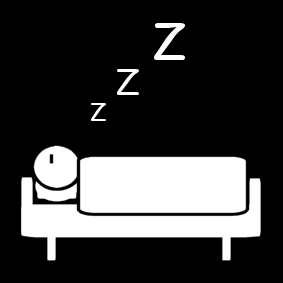
\includegraphics[width=0.85\linewidth]{{sclera/slapen}}
        \caption{`sleep'}
    \end{subfigure}
    \begin{subfigure}{0.22\textwidth}
        
\includegraphics[width=0.85\linewidth]{sclera/dansen}
        \caption{`dance'}
    \end{subfigure}
    \begin{subfigure}{0.22\textwidth}
        
\includegraphics[width=0.85\linewidth]{{sclera/geven}}
        \caption{`give'}
    \end{subfigure}
    \begin{subfigure}{0.22\textwidth}
        
\includegraphics[width=0.85\linewidth]{sclera/koken}
        \caption{`cook'}
    \end{subfigure}
    \caption{Simplex situations ('verbs' pictos)}
    \label{ex:sclera:simplex-situations}
\end{figure}

\begin{figure}[h]
    % \label{differentdogs}
    \centering
    \begin{subfigure}[t]{0.22\textwidth}
        
\includegraphics[width=0.85\linewidth]{{sclera/muziek-luisteren}}
        \caption{`listen' + `music'}
    \end{subfigure}
    \begin{subfigure}[t]{0.22\textwidth}
        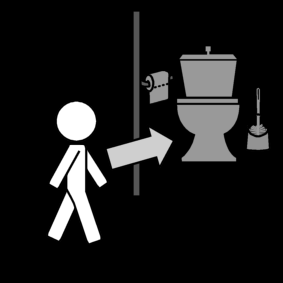
\includegraphics[width=0.85\linewidth]{sclera/toilet-gaan}
        \caption{`go (to)' + `bathroom'}
    \end{subfigure}
    \begin{subfigure}[t]{0.22\textwidth}
        
\includegraphics[width=0.85\linewidth]{sclera/koken-ik}
        \caption{`I' + `cook'}
    \end{subfigure}
    \begin{subfigure}[t]{0.22\textwidth}
        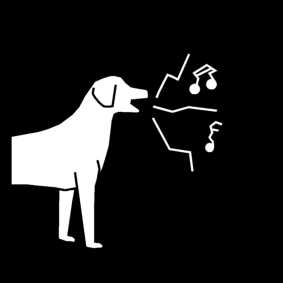
\includegraphics[width=0.85\linewidth]{sclera/hond-blaffen}
        \caption{`dog' + `bark'}
    \end{subfigure}
    \caption{Complex situations}
\end{figure}

\begin{figure}[h]
    % \label{}
    \centering
    \begin{subfigure}[t]{0.22\textwidth}
        \includegraphics[width=0.85\linewidth]{{"sclera/hij"}}
        \caption{`he/him'}
    \end{subfigure}
    \begin{subfigure}[t]{0.22\textwidth}
        \includegraphics[width=0.85\linewidth]{{"sclera/jij"}}
        \caption{`you (singular)'}
    \end{subfigure}
    \begin{subfigure}[t]{0.22\textwidth}
        \includegraphics[width=0.85\linewidth]{{"sclera/jullie"}}
        \caption{`you (plural)'}
    \end{subfigure}
    \begin{subfigure}[t]{0.22\textwidth}
        \includegraphics[width=0.85\linewidth]{{"sclera/spel mijn beurt"}}
        \caption{`mine'}
    \end{subfigure}
    \caption{`Pronominal' pictographs}
    \label{}
\end{figure}

\begin{figure}[h]
    % \label{}
    \centering
    \begin{subfigure}[t]{0.22\textwidth}
        \includegraphics[width=0.85\linewidth]{{"sclera/peper en zout"}}
        \caption{`salt and pepper'}
    \end{subfigure}
    \begin{subfigure}[t]{0.22\textwidth}
        \includegraphics[width=0.85\linewidth]{{"sclera/eten en drinken"}}
        \caption{`food and drink'}
    \end{subfigure}
    \begin{subfigure}[t]{0.22\textwidth}
        \includegraphics[width=0.85\linewidth]{{"sclera/baby zeep"}}
        \caption{`baby soap'}
    \end{subfigure}
    \caption{Complex entities (nominal compounds)}
    \label{}
\end{figure}

\begin{figure}[h]
    % \label{}
    \centering
    \begin{subfigure}[t]{0.22\textwidth}
        \includegraphics[width=0.85\linewidth]{{"sclera/jaloers boos"}}
        \caption{`jealous'}
    \end{subfigure}
    \begin{subfigure}[t]{0.22\textwidth}
        \includegraphics[width=0.85\linewidth]{{"sclera/blij"}}
        \caption{`happy'}
    \end{subfigure}
    \begin{subfigure}[t]{0.22\textwidth}
        \includegraphics[width=0.85\linewidth]{{"sclera/bed niet goed liggen 2"}}
        \caption{`bed uncomfortable'}
    \end{subfigure}
    \caption{Emotion/attitude}
    \label{}
\end{figure}

\begin{figure}[h]
    \centering
    \scriptsize
    \begin{subfigure}[t]{0.22\textwidth}
        \includegraphics[width=0.85\linewidth]{{"sclera/asbak 4 kruis rood"}}
        \caption{`no smoking' (red cross)}
    \end{subfigure}
    \begin{subfigure}[t]{0.22\textwidth}
        \includegraphics[width=0.85\linewidth]{{"sclera/aanraken ander kruis rood"}}
        \caption{`no touching others' (red cross)}
    \end{subfigure}
    \begin{subfigure}[t]{0.22\textwidth}
        \includegraphics[width=0.85\linewidth]{{"sclera/delen snoep groen"}}
        \caption{`share candy' (green)}
    \end{subfigure}
    \begin{subfigure}[t]{0.22\textwidth}
        \includegraphics[width=0.85\linewidth]{{"sclera/veiligheidsgordel zelf aandoen groen"}}
        \caption{`buckle seatbelt'  (green)}
    \end{subfigure}
    \caption{`Imperative' pictographs (directives)}
    \label{}
\end{figure}

\begin{figure}[h]
    % \label{}
    \centering
    \begin{subfigure}[t]{0.22\textwidth}
        \includegraphics[width=0.85\linewidth]{{"sclera/gelijke kansen"}}
        \caption{`equal opportunities'}
    \end{subfigure}
    \begin{subfigure}[t]{0.22\textwidth}
        \includegraphics[width=0.85\linewidth]{{"sclera/herhalen"}}
        \caption{`repeat'}
    \end{subfigure}
    \caption{Abstract concepts}
    \label{}
\end{figure}


Finally, the \sclera\ set includes a number of pictographs which are slightly
more marked. A first subset comprises opposition pairs. These often relate to
behaviour. In contrast to the rest of symbol set (with a few exceptions), these
pictographs make use of color: their (black) background is swapped out for
either a green or red one to indicate permission or prohibition, respectively.
Other pictographs, most of them `verbal', are marked for `positive' or
`negative' connotation on top of the concept that they depict, allowing the
user to express his attitude toward, for example, a situation of `saying
goodbye'. On a thematic level, the \sclera\ set contains a wide variety of
pictographs relating to independent living (bank cards, ATMs, taking the train,
etc.), culture, contemporary lifestyle and technology (electronic
communication, drugs, music), as well a number of `taboo' subjects such as
sexuality, religion, hygiene, and death.

\subsection{Choosing \sclera}
\label{sub:Beta}

\sclera\ is already used by the Picto2Text system \citep{sevens2015natural}, as
well as by its forerunner, the Text2Picto system
\citep{vandeghinste2015translating}, both introduced in
section~\ref{sub:picto2text}. As is discussed there, both translation systems
rely on previously established links between pictograph identifiers on the one
hand and WordNet synsets on the other \citep{vandeghinste2014linking}. (These
synsets are in turn linked to the EuroWordNet grid and SUMO ontology.) In order
to keep open the option of integration with the Picto2Text system further down
the road, as well as to enjoy the possible future benefits of the rich
lexical-semantic resource upon which its operation relies, the \depicto\ system
follows the Picto2Text example and adopts the \sclera\ set.

There are alternatives, however. Filtering these on availability (the operative
criterion being `free'), expressiveness, and success in user testing, the next
best option is the \emph{Beta} symbol set. The pictographs in this set make
much more use of color than those in \sclera, which, despite the resulting lack
of uniformity, makes them visually more appealing for some people. Aesthetics
aside, there are some important differences with the \sclera\ set. For one
thing, \emph{Beta} symbols depict only simplex concepts, as opposed to allowing
compounding and complexing. For another, prepositional relations are depicted.
While the first divergence makes little difference for compatibility with a
\sclera-oriented system, as \emph{Beta} can simply be treated as a subset of
the expressive scope of \sclera, the second difference makes things a little
trickier, since prepositional pictographs are not supported by the grammar of
\sclera\ which the \depicto\ system uses. For the time being, therefore,
\emph{Beta} is left to the side, although it is important to realize that it is
there, if only because it \emph{is} supported by the Picto2Text and Text2Picto
systems.

%-----------------------------------------------------------------------------
\section{Grammar engineering: The \delphin\ toolkit}
\label{sec:delph-in}

There are numerous grammar formalisms for which parsing and (slightly less
often) generation implementations exist. These include -- to name a few --
Context-Free Grammars (CFGs; \citet{chomsky1959certain}, Unification Grammars
(UGs; i.a. \citet{shieber1983formalism}), (Lexicalized) Tree-Adjoining Grammars
((L)TAGS; \citet{joshi1997tree}), and Dependency Grammars (DGs;
\citet{vater1975toward}). With the exception perhaps of traditional CFGs, each
of these formalisms has its merits. Additionally, their implementations vary in
the algorithms that they use, the degree to which these algorithms are
optimized, and the extent to which they have been designed with a
particular theoretical framework for syntactic analysis in mind. In short,
choosing a formalism is no easy task.

To keep things simple, therefore, both the analysis and generation modules
found in the \depicto\ system make use of the same unification-based formalism,
are written within the same framework, viz., \hpsg\ \citep{pollard1994head},
and rely on the same software for processing. These resources, each
representing multiple person-years of work, are all developed and distributed
by the same community: the \emph{Deep Linguistic Processing with HPSG
Initiative} (\delphin \footnote{http://moin.delph-in.net/}), an international
collaborative grammar engineering effort aimed at developing open-source NLP
tools for `deep' linguistic processing of human language. These tools can be
augmented with statistical processing methods, but the basis is thoroughly
symbolic. Through collaboration, with founding members coming from Stanford's
CSLI (USA), from Germany's DKFI and University of Saarland, and from Norway's
University of Science \& Technology and University of Oslo, the \delphin\
project has made it significantly more cost-effective to develop efficient
large-scale implemented grammars. It has also made the development process a
great deal more rewarding by providing a variety of specialized tools to
process grammars with, the most important relating to parsing, generation and,
as we shall see in the next section, the transfer of semantic representations
for translation and paraphrasing purposes. Some of these tools are intended for
production, and \delphin\ grammars and tools are already in place in a number
of commercial applications.

The intercompatibility of \delphin\ tools and \delphin\ grammars, even though
these are often developed independently of another, is due to the convergence
on a small set of common descriptive formalisms. The first such reference
formalism relates to the specific variant of typed feature structure logic
which all \delphin\ grammars are expected to follow. (Typed feature structures
form the primary data structure in \hpsg\ as well as the LFG and CG frameworks,
both of which, incidentally, are also compatible with the \delphin\ grammar
processors.) A second reference formalism is the Minimal Recursion Semantics
format for semantic representation, which generally forms the main output of a
\delphin\ parser, and from which \delphin\ grammars are able to generate. Both
these formalisms, as well as the declarative language used to implement them,
will be discussed in more detail in the course of the current section.

The following provides a brief introduction to the \hpsg\ framework, discusses
the \delphin-style typed feature structure (TFS) formalism in more detail, and
takes a look at the declarative specification language in which grammar files
are written (\tdl) as well as the way in which individual files combine to form
a complete HPSG grammar. After introducing the \mrs\ formalism for semantic
representation next, we turn to the \lingo\ Grammar Matrix starter-kit, which
provides the `core' for the grammars used by the \depicto\ system's analysis
and generation modules. Finally, the relatively recent \ace\ system is
introduced, an all-in-one \delphin\ grammar processor designed for speed and
efficiency, with support for transfer-based machine translation.

\subsection{Computationally implemented HPSG}
\label{sub:HPSG}

This subsection presents a lightning introduction to the framework of
Head-driven Phrase Structure Grammar (\hpsg) \citep{pollard1994head} and
describes the specific typed feature structure formalism used in \delphin\
implementations. To round off, it looks at the expected source file structure
of a typical \delphin\ and details a selection of common differences between
theoretical and computational variants of \hpsg.

\subsubsection{The basic theoretical framework} % or the formalism?

Head-driven Phrase Structure Grammar (\hpsg) is a strongly lexicalist, modular,
unification-based linguistic theory originally developed by Ivan Sag and Carl
Pollard in the mid-1980s \citep{pollard1994head}. Unlike transformational
grammars, it is entirely surface-oriented, and treats linguistic objects not as
trees, but as structured sets of constraints that can be modelled by means of
\emph{feature structures} (FSs) (informally: feature-value pairs; formally,
directed acyclic graphs). Within this model-theoretic approach, each linguistic
object, and thus each feature structure, is further seen as instantiating a
particular \emph{type}. The type to which a linguistic object belongs is
situated within a greater hierarchy of types. These are ordered from most
general to most specific according to the generality of the information, i.e.,
constraints, specified by the associated feature structure. This \emph{type
hierarchy} is used to capture both lexical and syntactic generalizations. The
constraining relation between types and their features is expressed by
\emph{typed feature structure descriptions}\footnote{The literature tends to
emphasize that there is a difference between these typed feature structure
descriptions and the typed feature structures (TFSs) which they describe
\citep{copestake2002implementing}. However, the difference is very subtle,
essentially boiling down to the fact that TFS descriptions place partial
constraints on possible models, whereas typed feature structures are understood
as maximally specific models that correspond to linguistic reality. Because of
this subtlety, particularly in an implementation-oriented context, where, prior
to compilation, grammars consist entirely of TFS \emph{descriptions}, I follow
\citet{copestake2002implementing}) in ignoring it except when it is absolutely
relevant.}, which are represented as attribute-value matrices (AVMs)
\citep{sag1999syntactic}.

To re-iterate the last paragraph slightly -- within the \hpsg\, framework all
linguistic objects are modelled as TFSs. On the linguistic level, the most
general type is that of the \emph{sign} (a tuple of phonological and
syntactic-semantic information) \citep{fokkens2014enhancing}, which has lexical
and phrasal signs as its subtypes. Lexical signs include lexemes and/or words.
Phrasal signs amount to the grammar rules that combine lexical or other
saturated phrasal TFSs (via the operation of unification) into larger
well-formed TFSs corresponding to immediate constituents. The principles that
determine both the syntactic and semantic well-formedness of these constituents
form an additional set of phrasal TFSs. As larger TFSs are built up (from a
parsing perspective), the phonological/orthographic information borne by
constituent TFS is appended, such that the root TFS, which is equivalent to the
root of a syntactic tree, contains the entire parsed string.

\begin{exe}[h]
    \ex\label{simpleTypeHierachy}Top of a typical \hpsg\ type hierarchy\\\\
    % 
\includegraphics[height=3cm]{placeholder}
    \begin{tikzpicture}[scale=0.9]
    \Tree [ .sign [
                    .{lexical sign}
                    word
                    lexeme
                  ]
                  [
                    .{phrasal sign}
                    {non-headed phrase}
                    {headed phrase}
                  ]
          ]
    \end{tikzpicture}
\end{exe}

True to its name, the \hpsg\ framework generally treats syntactic constituents
as consisting of a head structure and one or more sister structures which are
selected for by the head or, in some cases, select the head, but without
assuming its status. In terms of the valential relationship between the head
and non-head daughters of the mother node, the head-subject, head-complement,
head-specifier, and head-modifier rules are the most common, and most phrasal
rule types inherit from them. (Their names are sufficiently self-explanatory
for this purposefully brief introduction.) In order that the head of a
constituent is accessible to subsequent phrasal rules, its \textsc{head}
feature, which encodes syntactical features such as its part of speech, is
passed up by virtue of the Head Feature Principle \citep{sag2003syntactic},
which. The TFS through which this principle enters the grammar makes use of an
identity statement (notationally indicated with co-indexed variable tags) that
requires the value of the \textsc{head} feature of the mother TFS and the value
of the \textsc{head} feature of the head daughter TFS to be token-identical.
This mechanism of structure sharing is characteristic of \hpsg\, and, combined
with unification, accounts for much of its flexibility and elegance.

As a lexical theory, finally, \hpsg\ treats the lexicon as a rich and
structured object \citep{muller13hpsg-synopsis}. In order to avoid redundancy,
the type hierarchy includes a separate set of mostly unary lexical rules whose
`application' is constrained to TFSs of the type \emph{lexeme} and/or
\emph{word} (depending on the precise flavor of \hpsg\ one is working in).
These can be subdivided into inflecting/morphological/affixing rules and
non-inflecting/constant rules. While intuitively evident in theoretical
versions of \hpsg, the former, when implemented, requires additional machinery
which usually amounts to some form of regex substitution. Common examples of
usage cases for non-inflecting lexical rules include modification of the
valential requirements of a matrix verb in the passive voice and of a
ditransitive verb that can undergo `dative shift'. Unlike the rules discussed
above, lexical rules are less free as regards the order of their application,
particularly, as we shall see, when implemented, with inflecting rules always
coming before their inflecting counterparts (again, from the perspective of
parsing, that is).

%----------------------------------------------------------------------------

\subsubsection{The \delphin\ formalism of TFSs}
\label{ssub:delphin}

\delphin\ grammars consist of a specification of a type system and of various
typed feature structures (TFSs) which are to be inferred from this type system.
These TFSs, which function (among other) as grammar rules, lexical rules, and
lexical entries \citep{copestake2000appendix}, are considered well-formed on
the basis of a relatively conservative subset of the typed feature structure
logic described by \citet{carpenter1992logic}. This logic also forms the basis
of the machine-readable specification language in which \delphin\ grammars are
encoded: type-description language (\tdl) \citep{krieger1994tdl}. We will
return to \tdl\ shortly.

The selection of the \delphin\ formalism was guided by concerns about
linguistic adequacy grounded in \hpsg\ and about requirements for efficient
processing \citep{oepen2010disambiguate}. Informally, the formalism is
characterized as relating to a closed-world, multiple-inheritance type system
that enforces strong typing (i.e., every structure belongs to a type) and
strict appropriateness (i.e., all features a type can be defined for must be
introduced at some point in the inheritance hierarchy). At the same time, the
formalism allows types to be associated with arbitrarily complex constraints
(such as TFS embedding via structure sharing), which are inherited either upon
compilation or at runtime. The inheritance of constraints, moreover, is
monotonic, and features are introduced maximally, such that in instances of
multiple inheritance (which, to be clear, form the majority) from several
partial TFS descriptions, the result is always a unique most general structure,
i.e., a greatest lower bound. Compared to other variants of typed feature
structure logic, the \delphin\ formalism is very restricted. There is no room
for formal devices such as disjunction (which can lead to expensive
backtracking), negation, implication, inequality, default inheritance (this is
actually permitted, but rarely used), set-valued features and relational
constraints (e.g. `true' lists, which are implemented instead using the
mechanism of embedded feature-structures), and extensionality (anything that is
not in the grammar does not belong to the models which it can produce)
\citep{copestake2000appendix}. As a matter of fact, the only formal
device/operator which the \delphin\ TFS formalism uses is conjunction.

\paragraph{Type Description Language (\tdl)}
\label{par:tdl}

Set out in \citet{copestake2002implementing} (to date, still the best
introduction to \delphin-style grammar development), \tdl\ is the specification
language used to define types, their constraints, and their place in the type
hierarchy, i.e., in relation to their supertypes. \tdl\ descriptions always
have an AVM equivalent, as \cref{ex:avm-vs-tdl} shows for a non-linguistic
example. Feature structures are demarcated by opening and closing square
brackets. Feature names are conventionally written in uppercase, while their
values, which can be other types, are written in lowercase. If the value of a
feature is both a type \emph{and} and a more specific feature structure
appropriate to that type, then the two are separated by an ampersand (`\&') to
indicate conjunction/unification. Feature-value pairs are separated by commas,
and all \tdl\ descriptions must terminate in a period (`.'). Instead of using
boxed numbers, \tdl\ descriptions indicate structure sharing by means variable
names prefixed with a hashtag (or `octothorp', `pound sign', `\texttt{\#}').

\begin{exe}[h]
    \ex Equivalent AVM and \tdl\ descriptions for a (\textbf{non-linguistic}) typed feature structure
    \label{ex:avm-vs-tdl}
    \avmoptions{notactive}
    \small
    \begin{xlist}
        \ex AVM description\\\\
            % \scriptsize
            \begin{avm}
                \[ \asort{dog}
                   breed & \avmstring{Dalmation} \\
                   coat & \[ background & \@1 white \\
                             foreground & \[ \asort{spotted}
                                             SPOT-COLOR & black \] \] \\
                   fear & \avmstring{Cruela de Vil} \\
                   litter-size & more-than-100 \\
                   health-problems & \< \asort{deafness} \> \\
                   other & \[ favorite-camouflage-environment & \[ \asort{snow}
                                                         color & \@1 \] \] \]
            \end{avm}\\
            \vspace{0.5cm}
        \ex \tdl\ description
            \small
            \begin{verbatim}
dalmation := dog &
    [ BREED "dalmation",
      COAT [ BACKGROUND #camo-color & white,
             FOREGROUND spotted & [ SPOT-COLOR black ] ],
      FEAR  "Cruela de Vil",
      LITTER-SIZE more-than-100,
      HEALTH-PROBLEMS < deafness >,
      OTHER.FAVORITE-CAMOUFLAGE-ENVIRONMENT snow & [ COLOR #camo-color ] ].
            \end{verbatim}
    \end{xlist}
\end{exe}

\subsubsection{Components of a \delphin\ grammar}
\label{ssub:delphinstructure}

At the core of any \delphin\ grammar is its type hierarchy. This hierarchy can
be distributed over more than one \tdl\ file (e.g., for purposes of design,
debugging, clarity), but is interpreted by the grammar processor as building up
one large ontology of TFS descriptions.

The remaining components of the grammar are referred to as \emph{entries}. When
compiled or invoked by the processor, these give rise to maximally specific
typed feature structures. They comprise both rules and lexical entries. Once
again, these can be distributed over several \tdl\ files, but the processor
will interpret them accordingly. Phrasal rules are expanded upon compilation,
as are lexical rules, although these are treated separated so as to account for
the unique order-specific properties of the lexical rules, as well as the
intended behaviour of the phrasal rules, which, though specified as TFSs, are
interpreted as rewrite rules over other TFSs. Entries in the lexicon, finally,
are expanded at runtime rather than during compilation so as to keep down the
size of the compiled grammar. The configuration file associated with the
processor tells it how to interpret which components.

An small class of additional grammar entries is contributed by two files that
conventionally bear the names \texttt{roots.tdl} and \texttt{labels.tdl}.
\texttt{roots.tdl} contributes those TFSs that can function as start symbols in
the grammar, that is, as the root of a parse tree. \texttt{labels.tdl}
contributes the labels used to name the nodes in parse trees.

\subsubsection{Deviations from theoretical \hpsg}

While canonical theoretical \hpsg\ (which, for the sake of the discussion here,
I assume to be the flavor introduced in \citet{pollard1994head}) and
implemented \hpsg\ have, as one would expect, much in common, there are also
some differences in the analyses which they produce. These differences are relatively minor, but it helps to be aware of them nonetheless. The most salient, therefore, are briefly sketched out here.

\paragraph{Preference for unary or binary branching rules}
\label{par:naryvsbinary}

While the general phrasal rules, or `immediate dominance schemata'
\citep{pollard1994head}, of theoretical \hpsg\ generally license \emph{N-ary}
(viz., 1,2,3,4...n-ary) branching phrase structures \cref{ternary-branch}, such
rules are generally constrained to being either binary or unary in implemented
\hpsg. This is not to say that ternary, quaternary, etc. branching is ruled
out; it is simply dispreferred, as it leads to a significant increase in the
size of the search space that the parsing and generation algorithms need to
consider. The traditional analysis of the ditransitive valence schema of a verb
such as \emph{give} is instead analysed as two successive `applications' of
a binary head-complement rule, as in \cref{binary-branch}.

% uses qtree or tikz-qtree-compact
\begin{exe}
    \ex Ternary vs. binary branching analyses of ditransitive verb phrase (VP)\\
        \begin{xlist}
        \ex \label{ternary-branch} Ternary branching VP analysis\\
        \Tree [ .S
                     \qroof{the gorilla}.NP
                    [ .VP [ .V gave ]
                           \qroof{the scientist}.NP
                           \qroof{a hug}.NP
                    ].VP
              ].S\\
        \ex \label{binary-branch} Binary branching VP analysis \\\\
        \Tree [ .S
                    \qroof{the gorilla}.NP
                    [ .VP [
                            .VP [ .V gave ].V
                                  \qroof{the scientist}.NP
                                ].VP
                            \qroof{a hug}.NP ].VP
              ].S
        % \vspace{1cm}
        \end{xlist}
\end{exe}

\paragraph{Lists as feature structures}
% \label{par:paragraph label}

In theoretical \hpsg, lists are expressed as comma-separated items between
large angle brackets. While \tdl\ contains syntactic sugar that mimics this
notation, the underlying implementation of the list, however, is that of a
recursive typed feature structure consisting of a \emph{head} (\textsc{first})
and a \emph{tail} (\textsc{last}), which can have as its value a terminating
\emph{nil}, any single type, or another list with the same constraints.

\begin{exe}
    \ex\begin{xlist}
        \ex Traditional AVM notation used for lists:\\\\
            \begin{avm}
                [ fruits & < \textnormal{`oranges'}, \textnormal{`bananas'}, \textnormal{`apples'} > ]
            \end{avm}\\
        \ex Underlying structure of list, as made explicit in
                 implementations\\\\
            \begin{avm}
                [ fruits & [ first & \textnormal{`oranges'}\\
                             rest & [ first & \textnormal{`bananas'} \\
                                      rest & [ first & \textnormal{`apples'} \\
                                               rest & *end* ]]]]
            \end{avm}\\
    \end{xlist}
\end{exe}

Logics sets, which theoretical \hpsg\ indicates using a special curly brackets
notation, are treated within the \delphin\ formalism as simple lists. That is,
the items of the set are treated as having a particular order.

Finally, lists which are appended during the construction of larger TFSs (e.g.,
lists of semantic predications, the value of the feature bearing
orthographic/phonological information about the parsed/generated string, etc.)
are implemented as special kind of list, namely, a \emph{difference list}. We
do not need to get into the details of how this separate type of list is used
within the grammar, but it is useful to know that \tdl\ includes special
syntactic sugar that allows lists of this kind to be written as \texttt{<! [
LIST-ITEM ] !>}.

\paragraph{No Lexeme-word distinction}
% \label{par:paragraph label}

Some flavors of \hpsg\ posit a distinction between lexemes on the one hand and
the words which these lexemes instantiate on the other. As a result, one or
more constant lexical rules are required to \emph{pump} non-inflecting lexemes
to the word level. This distinction is perfectly compatible with the \delphin\
framework, yet it is rarely adopted. In \delphin-grammars lexemes and words
tend to be synonymous. This is certainly the case for the grammars developed in
this thesis.

\paragraph{\emph{Greatest lower bound} requirement}
% \label{par:paragraph label}

Multiple type inheritance is as powerful a mechanism in theoretical \hpsg\ as
it is in implemented \hpsg. However, while theoretical variants, generally for
illustrative purposes, show multiple same-level types inheriting from the
\emph{same} supertypes, this is not allowed in the more strictly formalized
type system found in implemented \hpsg: in cases of multiple inheritance, types
must share a unique most general type, or \emph{greatest lower bound (glb)}. In
large-scale implemented grammars, this generally leads grammar writers to
specify intermediate types that, in a purely theoretical framework, may be seen
as redundant. While this well-formedness condition on the type hierarchy is
clearly not trivial, failing to take it into account does not immediately
undermine the grammar either, as most grammar processors possess additional
machinery to add missing \emph{glbs} to the type hierarchy.

\begin{exe}[h]
    % \captionsetup[subfigure]{margin=20pt}
    % \centering
    % \begin{subfigure}[b]{0.45\textwidth}
    \ex
        % \centering
        \begin{xlist}
        \tikzset{every tree node/.style={anchor=base}}
        \ex Hypothetical example of multiple inheritance in \emph{theoretical}
                 \hpsg \vspace{0.5cm}\\
            \begin{tikzpicture}
                \Tree [.*top*
                        [ . \node (a) {a};
                            c
                           [ . \node (d) {d}; ] ]
                        [ . \node (b) {b};
                            [ . \node (e) {e}; ]
                             f ] ]
                             %  \edge[draw=none]; {} \edge; {B} ]]]]
                \draw (a.south) -- (e.north);
                \draw (b.south) -- (d.north);
            \end{tikzpicture}
        \ex\label{ex:inheritance-with-glb}
            Multiple inheritance in \delphin, with additional
                 \emph{greatest lower bound} (\emph{glb}) type \vspace{0.5cm}\\
            \attop{\begin{tikzpicture}
                \tikzset{every tree node/.style={anchor=base}}
                \Tree [.*top*
                        [ . \node (a) {a};
                            c
                            \edge[draw=none]; {}
                           [  .\node (glb) {\emph{glb}};
                                d
                                e  ] ]
                        [ . \node (b) {b};
                            % \edge[draw=none]; {}
                            \edge[draw=none]; {}
                             f ] ]
                \draw (b.south) -- (glb.north);
            \end{tikzpicture}}
    \end{xlist}
\end{exe}

%-----------------------------------------------------------------------------

\subsection{Minimal Recursion Semantics (\mrs)}
\label{sub:mrs}

\delphin\ grammars are designed to map bi-directionally between surface strings
and semantic representations. These representations are encoded as TFS and
correspond to descriptions used within the formalism of Minimal Recursion
Semantics (\mrs) \citep{copestake2005minimal}. This formalism, which aims to
provide a framework for computational semantics that is suitable for both
parsing and generation, serves as theory-agnostic meta-language for more
traditional semantic formalisms such as predicate calculus and generalized
quantifiers (which are common in \delphin\ grammars). \mrs\ abstracts away from
surface syntactic structure and undecidable scope ambiguities by means of
characteristically flat (i.e., non-recursive) representations that use explicit
pointers to encode argument structure and scope effects
\citep{copestake2000open}. The resulting potential for underspecification
recommends \mrs\ to computational applications that, like the one developed
here, require robust generation. Despite its close ties to the \delphin\
project, \mrs\ has also become popular among theoretical \hpsg\ researchers as
well as among researchers working within non-\hpsg\ frameworks such as TAG,
CxG, and LFG. In the remainder of this subsection, we take a closer look at the structure of the representations themselves.

\subsubsection{Make-up of an \mrs\ structure}

An \mrs\ structure (sometimes abbreviated, somewhat confusingly, to `\mrs')
essentially consists of three parts: an index/indices, a bag of elementary
predications, and a set of handle constraints. Each is explained briefly here
with reference to the example \mrs\ representation for the sentence \emph{Every
brown dog barks} shown in \cref{ex:basicmrs}.

% \todo[inline]{I refer to the HOOK feature, but this is only used within the grammar. \mrs\ representations flatten this out. or so it seems right now. unsure what to do.}

% \begin{minipage}[t]{\linewidth}
\begin{exe}
    % \centering
    % 
\includegraphics[height=3cm]{placeholder}
    \nolistbreak
    \ex\label{ex:basicmrs}
    \mrs\ representation of \emph{Every dog barks}\\
    % \begin{minipage}{\linewidth}
    % \noindent
    \avmvalfont{\small}
    \begin{avm}
        % \avmvskip{.1ex}\avmhskip{.5em}
        [ \asort{mrs}
            hook & [ \asort{hook}
                     ltop & \avmbox{h0} \\
                     index & \avmbox{e2} ] \\
            rels & < [ \asort{ep}
                       lbl \avmbox{h4}  & \\
                       pred & \avmstring{every\_q\_rel} \\
                       arg0 & \avmbox{x3}  \\
                       rstr & \avmbox{h5} \\
                       body & h6 ],
                     [ \asort{ep}
                       lbl & \avmbox{h7} \\
                       pred & \avmstring{dog\_n\_rel} \\
                       arg0 & \avmbox{x3} ],\\
                      [ \asort{ep}
                       lbl & \avmbox{h1} \\
                       pred & \avmstring{bark\_v\_rel} \\
                       arg0 & \avmbox{e2} \\
                       arg1 & \avmbox{x3} ] > \\
            hcons & < [ \asort{qeq}
                        harg & \avmbox{h0} \\
                        larg & \avmbox{h1} ],
                      [ \asort{qeq}
                        harg & \avmbox{h5}  \\
                        larg & \avmbox{h7} ] > ]
    \end{avm}

\end{exe}
% \end{minipage}

\paragraph{Elementary predications}

The primary units of information in an \mrs\ representation are its
\emph{elementary predications (EPs)}. Each \emph{EP} consists of a named
relation (or predicate) and any number of associated arguments, conventionally
labelled ARG\emph{N}. The values of these arguments are logical variables and
belong either to the type \emph{event} (\emph{e}) or
\emph{entity/individual/referential index} (\emph{i}). These logical variables
establish links across EPs. They can also encode for additional \emph{variable
properties} relating, among other, to tense, aspect, illocutionary force,
person, number, or gender, depending on whether the variable relates to an
event or to an entity. Additionally, all EPs have a unique distinguished
argument \textsc{arg0} which, informally, function as a sort of index to the
predicate itself. Generally, the \textsc{arg0} of the main predicate forms the
top index of the \mrs\ representation (found under \textsc{hook|index}) Within
the \delphin\ TFS geometry, EPs are generally found under the feature
\textsc{rels}. Although they formally form an unordered bag (i.e., do not have
fixed order or require uniqueness), they are implemented as ordered lists.

\paragraph{Handle constraints}

In order to capture scopal information, \emph{labels} are introduced (on the EP
feature \textsc{LBL}) with a so-called \emph{handles (hN)} as their values.
These handles form the values of scopal arguments (e.g. \textsc{rstr} and
\textsc{body}), in which case they are sometimes referred to as \emph{holes},
the highest scoping EP shares its handle with the \emph{hook} feature
\textsc{ltop} (\emph{local top}), and EPs that have the same handle are
interpreted as conjuncts.  In a well-formed \mrs, handles can be identified (in
one or more ways) such that the dependencies between EPs form a tree. Constraints on possible interpretations of scopal relations are introduced under \textsc{hcons}. Here, the type \emph{qeq (equality modulo quantification)} is used to indicate that either the value of \textsc{larg} \emph{l} fills the hole \emph{h} in \textsc{harg}, or that \emph{l} is indirectly linked to \emph{h} via one or more \emph{floating quantifiers} (for which the reader is referred to \citet{copestake2005minimal}). In both cases the effect is to convey that one handle outscopes another.

\paragraph{Hooks}

Already mentioned above, the features \textsc{index} and \textsc{ltop} belong
to the type \emph{hook}. The function of this type is to `publish' those parts
of the EP list that the grammar's rules need access to when building up
semantic representations. Generally, these parts include the index of the head of the current phrase and the identity of the highest-scoping handle. There are several other features which \emph{hook} can be specified for, but these are not discussed here. As far as semantic composition in the \depicto\ system is concerned, knowledge of \textsc{index} and \textsc{ltop} is sufficient.

%-----------------------------------------------------------------------------

\subsection{The \lingo\ Grammar Matrix starter kit}
\label{sub:lingomatrix}

Designing large-scale TFS grammars from scratch is hard work, regardless of the
precise formalism, implementation or framework used. In fact, as
\citet{Ben:Fli:Oep:02} point out, the most extensive \delphin\ grammars to
date, viz., the English Resource Grammar (ERG; \citep{copestake2000open}),
the Jacy grammar of Japanese \citep{siegel2002efficient}, and the German
Grammar (GG) \citep{muller2000hpsg}, each required between 5 and 15 years of
development by experts before being ready for use in real-life applications;
and some, such as the ERG, are still undergoing refinement. This lengthy and
costly development process is -- or, rather, \emph{was} -- largely due to the
fact that, while these grammars use the same formalism and framework, they were
developed more or less independently of each other, resulting in time being
spent on design problems (e.g., the structure of the type hierarchy, the HPSG
feature geometry, the implementation of semantics as well as technical devices
such as lists and `appends' -- to name a few), for which compatible solutions
had already been devised. As an alternative to the cycle of wheel re-inventing,
\citet{Ben:Fli:Oep:02} present the first version of the \lingo\footnote{The
CSLI (Stanford  University) Linguistic Grammars Online (\lingo) laboratory is
one of the main founders of the \delphin\ project} Grammar Matrix starter kit
(it has evolved considerably in the years since, undergoing several refactoring
stages), a language-independent grammar resource designed to facilitate both
the initial and long-term development of grammars written in the \delphin\
formalism. At its core, the starter kit comprises a set of typologically
agnostic generalizations across the largest \delphin\ grammars, including
definitions for basic linguistic objects, common best practices (e.g., type
naming conventions), and analyses that adequately generalize to other
languages. The idea is for new \delphin\ grammars\footnote{A slight
anachronism, as the \delphin\ project did not take off until later} to be able
to build on top of this core, i.e.,  by inheriting from it and adding more
specific constraints until (a subset of) the grammatical requirements of a
given language are met. The remainder of this section takes a slightly closer
look at the Matrix, its core in particular, and introduces the script-based
customization system that its developers have since devised in order to make
prototyping with it even faster.

\subsubsection{Inside the Matrix}
\label{ssub:matrixcore}

As a starter kit, the Grammar Matrix includes all the components needed to
construct a \delphin\ grammar (see section~\ref{ssub:delphinstructure}). The
most important component is a file called \texttt{matrix.tdl}, which defines
the top of the grammar's TFS hierarchy. Aspects of the grammar that have been
defined here since the first version of the Matrix \citep{Ben:Fli:Oep:02}
include the general feature geometry of signs, technical devices (e.g., list
manipulation), basic lexical and phrasal rule types (both unary and binary),
headed and non-headed rule types, phrase-internal order rule types (e.g.,
head-left and head-right), constructions corresponding to the \hpsg\ schemata
(i.e., Head-Subject, Head-Complement, Head-Specifier, and Head-Modifier
rules\footnote{Note that the flavor of \hpsg\ used in the \lingo\ Matrix does
not follow proposals to roll the Head-Modifier and Head-Specifier schemata into
a single \emph{head-functor} rule, as in \citet{vaneynde1998immediate} }), all
of them underspecified for word order. The \texttt{matrix.tdl} file, finally,
includes a semantic component, where a hierarchy of \mrs\ relation types is
defined, as well as types and constraints for the propagation of semantic
information throughout the phrase structure tree, a representation of
illocutionary force, and rule types allowing grammar rules to make semantic
contributions \citep{Flickinger:Ben:03}.

For the most part, the definitions in \texttt{matrix.tdl} were originally based
on those found in the English Resource Grammar (ERG). In order to make the
Matrix as language-independent as possible, however, the Japanese grammar Jacy,
a smaller grammar for Spanish, and general knowledge about typological
variation were used to guide decisions about which definitions to keep, discard
or underspecify \citep{Ben:Fli:Oep:02,fokkens2011metagrammar}. An example of
the latter is the separation of rules concerning immediate dominance (i.e.,
constituent structure) on the one hand and linear precedence (i.e.,
constituent-internal ordering) on the other. Several large-scale grammars have
been constructed using the original Grammar Matrix. These include grammars for
Norwegian, Spanish, Modern Greek, Portuguese, Korean, and Huasa
\citep{fokkens2014enhancing}. Based on feedback from developers working with
increasingly diverse languages, the Matrix has already undergone several update
cycles. In order to bring new improvements to existing Matrix-based grammars,
several script-based tools have been developed that modify all the components
of a given grammar to reflect changes in the updated Matrix core, such as -- in
recent years -- the introduction of \emph{disjunctive head types}. The problems
which these scripts have to overcome are by no means trivial.

Also included with the Matrix starter kit, finally, are configuration and
parameter files for easy start-up with a number of \delphin\ processors.
Originally, these were just for the \lkb\ grammar engineering environment
\citep{copestake2002implementing}, but recent versions of the Matrix also
support the \ace\ system \citep{sweaglesACE} and the \textsc{pet} parser. The \lkb\ and \ace\ systems are introduced in section~\ref{sub:ace}.

\subsubsection{The customization system}
\label{ssub:matrixcustomization}

By providing a solid, language-independent foundation, the Grammar Matrix
significantly reduces the initial cost of and level of expertise needed for
developing new processable grammars, which, as explained above, essentially
extend the core grammar to cover the specific phenomena and properties of a
given language. Drawing on experience teaching students \footnote{Since 2004,
the Grammar Matrix has been used in a grammar engineering course taught at the
University of Washington (http://courses.washington.edu/ling567/)} to use the
Matrix, its developers notice that parts of this process of extension can be
automated \citep{bender2007combining}. Language-specific analyses of
crosslinguistically variable phenomena are not implemented manually, but
parameterized and generated by a script, or rather, \emph{several} scripts,
each representing a so-called \emph{module} (today: \emph{libary}). First
proposed in \citet{bender2005rapid}, this approach formed the basis for the
Grammar Matrix customization
system\footnote{http://www.delph-in.net/matrix/customize/matrix.cgi}
\citep{bender-EtAl:2010:Demos}. The customization system uses a web-based
questionnaire to dynamically (i.e., adapting the HTML code based on other
answers) elicit information from users about the language they want to model.
This information corresponds to the modules for basic word order, yes-no
questions, sentential negation and lexical items, including nouns, transitive
and intransitive verbs, auxiliaries, determiners, negation markers and case
marking adpositions. Input from the questionnaire is stored in a \emph{choices}
file. Once validated, i.e., when no inconsistencies or missing information are
identified, the choice file is passed to the customization script, which
creates an initial custom grammar. The user can test this grammar remotely by
generating sentences with it. If these are all or mostly grammatical, the user
can choose to download the complete grammar. From that point on the grammar
behaves like any other \delphin\ grammar. (For a clear and relatively
up-to-date overview of the system in its entirety, please see
\citet{fokkens2014enhancing}, whose research on `Metagrammar engineering' is
largely based on the idea of script-based grammar generation.) As
chapter~\ref{chap:pipeline1} explains in more detail, both the \depicto\
system's grammars stem from a simple SVO-language grammar that was initially
set up with the aid of the customization system.

%-----------------------------------------------------------------------------

\subsection{The \ace\ processor}
\label{sub:ace}

The \delphin\ repository includes a number of ready-made made tools for
parsing\footnote{for a visual comparison see
http://sweaglesw.org/linguistics/delphin-engines.html}, two of which, viz., the
\lkb\ \citep{copestake2002implementing} and the \ace\ \citep{sweaglesACE}
system, additionally support generation as well as semantic transfer (the
latter introduced in the next section (\ref{logon}). The \lkb\ was originally
designed as a tool for grammar development, serving as a so-called \emph{GDE}
(a play on \emph{IDE}\footnote{(Integrated Development Environment)}). The
\ace\ system, by contrast, was developed for speed. It uses the same processing
algorithms as the \lkb\ (barring a handful of optimization techniques), but
performs about 15 times faster \citep{sweaglesACE}. Since users tend to like
their translation tools as responsive as possible, the \ace\ processor is the
obvious choice for deploying such systems in production. As far as the grammar
development process is concerned, here, too, the \ace\ processor has proven
itself to be a suitable tool. The remainder of this subsection introduces the
\ace\ system in slightly more detail and explains how it can be used for
effective grammar development as well. Before we proceed, however, it ought to
be said that, while the following does include details about parsing and
generation algorithms, the \ace\ system is to all intents and purposes treated
as a `black box' within the \depicto\ system. It does what it promises, and it
does it well; but its codebase and API, both written in C, are best left to the
more initiated.

The Answer Constraint Engine\footnote{http://sweaglesw.org/linguistics/ace/}
(\ace) \citep{sweaglesACE} is a \emph{relatively} recent addition to the
open-source \delphin\ ecosystem. Initial development, which began in 2004, was
for proprietary uses, and the software was not openly released until 2011
(under the open-source MIT license). Although essentially a one-man project,
the \ace\ processor is still actively being developed, as its release notes
suggest\footnote{http://sweaglesw.org/linguistics/ace/download/RELEASE-NOTES-0.9.20},
as does the \delphin\ wiki, which hosts an up-to-date wish list of improvements
that other developers would like to see incorporated. \ace\ runs on GNU/Linux
systems and stands out as being the \emph{only} \delphin\ processor that also
supports Mac OS X (my main development environment). Interacting with the
system, which is available as a ready-made binary, is done via the command
line. Both the inputs and outputs are plain text. In parsing mode, \ace\ takes
as input a stretch of text and outputs, if possible, one or more \mrs s. In
generation mode, it takes as input an \mrs\ and outputs one or more instances
of generated text. In \emph{transfer mode} (i.e., the `bridge' in
transfer-style rule-based translation systems, this concept introduced in the
next section), both the input and the output are \mrs s. One of the many
practical advantages of the \ace\ system is that the output of given mode can
be passed, if appropriate, to the input of an arbitrary mode: multiple calls to
the \ace\ binary can be chained easily by means of Unix `pipes' (i.e., {\texttt
|}'s).

For parsing, the \ace\ system uses a classic, agenda-driven chart parser, based
on Kay 1986 \citep{crysmann2012towards}. To be precise, this is a variation on
the bottom-up Cocke–Younger–Kasami algorithm, which is also used by other
\delphin\ processors. \ace\ also comes with REPP support (\emph{Regular
Expression Pre-Processing}) and built-in part-of-speech tagging. (These
features are of less use to the more predictable input expected by the
\depicto\ system.) For generation, \ace\ uses a chart generation algorithm
described in \citet{carroll1999efficient}. The input to the generation system
is a grammar and the semantics of the utterance to be generated (expressed in
\mrs). The generator's output is the list of \emph{all} strings which are
related to the input \mrs\ by the grammar. The generation process happens in
three stages: lexical-lookup (entries with corresponding predicate name values
are retrieved from the lexicon and instantiated on the chart generator); chart
generation; and modification insertion (whereby morphological lexical rules are
finally applied) \citep{fokkens2014enhancing}. Two efficiency measures are
taken to ``combat the exponential worst-case complexity of the chart generation
algorithm'' (i.e., if the input \mrs\ is too underspecified)
\citep{crysmann2012towards}. Described in \citet{carroll2005high}, these are
\emph{Ambiguity packing under subsumption} and \emph{Index accessibility
filtering}. My knowledge of parsing and generation techniques is too limited to
provide an adequate explanation of these. Therefore, please see the related
work instead. For transfer, the \ace\ system uses the \logon\ \mrs-rewriting
machinery. This is explained in the next section.

\subsubsection{Why not the \lkb, and how to use \ace\ for development}
\label{lkbvace}

On paper, the \lkb\ jumps out as the most suitable tool for designing and
debugging \delphin-style grammars. Not only does it include a graphical user
interface, it also provides a rich set of tools for visualizing various
components of the grammar, such as the type hierarchy, instantiated TFSs, parse
trees, generated trees, and parse/generation charts -- to name the most useful.
Particularly useful in the context of debugging is  ability to interactively
step through the parse chart. However, in developing the \depicto\ system, I
found the \lkb\ lacking in a number of respects. In the first place, its GUI is
relatively outdated by modern design standards, does not render well on HiDPI
screens, and its reliance on the CLIM (Common-Lisp Interface Manager) library
restricts its portability to Linux, 64-bit versions of which have additionally
to deal with the problem of missing 32-bit dependencies. The alternative is to
interact with the \lkb\ via its Lisp console. This console runs in, but behaves
very differently to, a standard Unix shell/terminal, and is only really usable
through mediation of the \emph{Emacs} text editor. In other words, in order to
circumvent the \lkb's GUI one must have some knowledge of Lisp (which I do not
to a sufficient degree) and one must be comfortable working with Emacs
(something of a presumption, given the wide range of capable text editors
available nowadays). And yet, unless one is able to circumvent the GUI, simple
tasks such as reloading (recompiling) a grammar, much less multiple grammars at
the same time, become highly repetitive and time-consuming. Setting up a
machine-translation system of the kind developed here \emph{is}
possible\footnote{http://moin.delph-in.net/MtSetup}, but it requires three
separate \emph{Emacs} windows running a separate \lkb\ session each and a fair
amount of additional Lisp code, leaving a fair amount of room for error. The
process is so convoluted, in fact, that I was able to get it working
\emph{once}.

Fortunately, the \ace\ system can be set up so as to get much of the same
visualisation functionality that makes the \lkb\ so useful. For this, the
LUI\footnote{http://moin.delph-in.net/LkbLui} (Linguistic User Interface)
application is required. Once downloaded and installed on the PATH, it allows
\ace\ to start up in so-called \emph{LUI mode} in combination with any of its
three other modes \footnote{http://moin.delph-in.net/AceLui}. In this mode,
\ace\ can instantiate visual browsers for constituent trees, feature
structures, \mrs s, parse charts, and local supertypes and subtypes. Unlike the
\lkb, \ace-in-LUI-mode is not able to visualize the entire type hierarchy. This
is not really a limitation, however: when dealing with large-scale grammars,
there inevitably comes a point when the type hierarchy simply becomes too big
to be visualized informatively. In comparison to the \lkb, LUI mode also adds
some new features, the most useful of which is drag-and-drop interactive
unification. Combined with the LUI application, as well as a smattering of
simple ad hoc bash script here and there, the \ace\ system becomes every little
bit as useful for grammar development as the \lkb, if not more.

%%%%%%%%%%%%%%%%%%%%%%%%%%%%%%%%%%%%%%%%%%%%%%%%%%%%%%%%%%%%%%%%%%%%%%%%%%%%%%

\section{Transfer-based MT: the \logon\ approach}
\label{logon}

As explained in \cref{sec:delph-in}, \delphin\ grammars are designed for both
parsing and generation, bi-directionally mapping between surface strings and
semantic representations (in the \mrs\ format; see section~\ref{sub:mrs}). This
bidirectionality has many uses. For example, it is possible to check whether a
given grammar is prone to overgeneration (i.e., is not sufficiently
constrained) simply by letting it generate from an \mrs\ obtained by parsing
with the same grammar. (The \ace\ processor, with its support for `pipes',
makes this particularly easy to set up (see section~\ref{sub:ace}).) A more
advanced application, which is developed here, similarly involves chaining the
parsing and generation steps, but uses \emph{different} grammars for each,
which has the effect of translating the input surface string into a
semantically equivalent string licensed by a different grammar. This comes
fairly close to the essential function of a rule-based machine translation
(RB\textbf{MT}) system. However, this approach is somewhat simplistic, since
the output of an RBMT system's \emph{source-language} grammar is generally not
compatible with its \emph{target-language} grammar, i.e., the grammar used for
generation. In the present case, the challenge consists in the fact that the
\mrs\ framework is not intended to be used as an \emph{interlingua}
\citep{copestake2005minimal}: \mrs\ representations are structurally codified
with regard to a number of conventions, but their semantic content (viz., the
(lexicalized) predicate names found on their list of \emph{Elementary
Predications}; see section~\ref{sub:mrs}) is largely language-specific. Since
interlinguas are, in fact, rare, most RBMT systems make use of an intermediate
\emph{transfer} component, which mediates between the output of the source
grammar and the input to the target grammar, transforming as required the
(semantic and/or syntactic) data structures passed between them
\citep{vandeghinste2008hybrid}.

For \delphin-based machine translation systems,
an open-source \mrs-oriented transfer mechanism is already available.
Originally developed within the context of the \logon\ Norwegian-English MT
project \citep{Lonning04logon.a}, this system rewrites \mrs s step by step
until one or more \mrs s are derived from which a target-language grammar can
generate. The rewrite process itself is determined by a set of bilingual rules
defined in a \emph{transfer grammar} \citep{oepen2008transfer} for a given
language pair. Implementations of the transfer engine are found in both the
\lkb\ and (since recently) the \ace\ processor (introduced in
section~\ref{sub:ace}).

The rest of this section takes a closer look at the \logon\footnote{\logon\ may
be understood as a branch of the \delphin\ consortium. For just over a decade,
it has worked on developing a hybrid machine translation infrastructure
suitable for \mrs-oriented grammars. The project started off as a collaboration
among three Norwegian universities, although it has since attracted developers
from other areas.} transfer system. First, it provides an informal introduction
to the general formalism for \mrs\ rewriting, focusing on those characteristics
of the formalism that are best kept in mind when developing a transfer grammar,
and gives a schematic description of the rewrite rules that constitute this
type of grammar. Next, we see how these rules are implemented descriptively,
namely, as typed feature structures, and how this benefits the internal
organisation of the transfer grammar. The last subsection shows how this
\emph{object-oriented} style of organisation makes it possible for developers
to provide resources that can serve as starter kit for the development of new
transfer grammars, in much the same vein as the \lingo\ Grammar Matrix (see
section~\ref{sub:lingomatrix}), albeit in a more rudimentary form. For the sake
of clarity, finally, it should be observed that the \logon\ transfer system
forms merely one part of the larger \logon\ MT
infrastructure\footnote{http://moin.delph-in.net/LogonTop}. The complete system
combines a symbolic basis with stochastic extensions, which provide, inter
alia, probabilistic rankings in the parse, transfer, and generation components,
as well as fallbacks for when the transfer system fails (\citet{bond2011deep},
\citet{Oepen02lingoredwoods}).

%-----------------------------------------------------------------------------

\subsection{\mrs\ rewriting}

The \logon\ transfer formalism provides a special-purpose graph rewriting
system\footnote{Formally, \mrs\ structures constitute \emph{directed acyclic
graphs} (for more detail, see section~\ref{sub:mrs})} in which individual
unification-based rewrite rules relate parts of a source-language \mrs\ to the
corresponding parts of a target-language \mrs\ \citep{oepen2008transfer}. This
is a stepwise process, with rewrite rules applying in the order in which they
are specified in the transfer grammar, as well as `consuming' their input,
i.e., replacing it with the corresponding target-language \mrs. As a result,
the application of each rule ``changes the `state of the universe' visible to
subsequent rule applications'' \citep{oepen2008transfer}. (This contrasts with
the phrasal and lexical rules encountered in the previous section, which
`combine' rather than `consume' their daughters, and, in fact, imposes upon the
transfer grammar the requirement that rules be ordered in increasing
specificity, so that more general rules are applied first.) In fact, the
structures manipulated throughout most of the transfer process consist of a mix
of the source-language \mrs\ and the target-language \mrs. The input and output
specifications of individual rules can access arbitrary structural properties
of the \mrs\ graph, as well as establish bindings via structure sharing, by
means of which properties can be `carried over' from the input to the output.
Because an \mrs\ can contain multiple parts for which the same rule is
relevant, rule application in the \logon\ system is not only ordered, but
breadth-first (i.e., all possible applications of a given rule are considered
before moving on to the next rule). Finally, to allow for the inverse
situation, that is, where multiple (possibly optional\footnote{Rewrite rules
can be marked for optionality. This is useful when dealing with an \mrs\
fragment that has several possible translations. Optional rules, which causes
the rewrite process to `fork' into parallel branches, are generally provided as
a series. The last rule in this series is marked as non-optional so as to
terminate it \citep{oepen2008transfer}.}) rules apply to the same \mrs\
fragment, the system supports backtracking \citep{oepen2008transfer}.

Turning to the rewrite rules themselves, which are referred to to as
\emph{\mrs\ Transfer Rules} (or \mtr s), these constitute four-tuples of
(partial) \mrs\ descriptions which correspond, as schematized in
(\ref{ex:mtr-schematic}), to the rule's \emph{Input}, \emph{Output}, and
two optional components that condition the applicability of the rule either by
constraining it with additional \emph{Context}ual information, or by blocking
it entirely by means of a \emph{Filter} \citep{oepen2008transfer}.

\begin{exe}
    \ex\label{ex:mtr-schematic}
        $[Context] \enspace Input \enspace [Filter] \enspace
        \longrightarrow  \enspace Output$
\end{exe}

The general idea is that, for an \mtr\ to be applied, the \mrs\ description
provided by its \emph{Input} component must be compatible with the \mrs\
(structure) currently being processed by the system. (This can be either the
original \mrs\ input to the transfer system or an intermediate structure
obtained from earlier \mtr\ applications.) If the partial \mtr's \emph{Input}
component can be unified with this \mrs\ (that is, if the the two \mrs\ graphs
can be structurally aligned), then the transfer rule is invoked, or `fired'.
The unified (aligned) substructures are consumed, and the \mrs\ description on
the \emph{Output} component specifies what to insert in their place
\citep{oepen2008transfer}. Those parts of the transferred \mrs\ which are not
aligned with the rule's \emph{Input} are not affected by it.

Originally built as an extension of the \lkb\ system (introduced in section
\ref{sub:ace}), the \logon\ transfer system describes \mtr s as typed feature
structures (TFSs, see \ref{ssub:delphin}). Accordingly, transfer grammars,
which may be understood as ordered sequences of \mtr\ descriptions, are written
in the \tdl\ specification language\footnote{Upon which the \logon\ system, in
fact, builds, adding syntax for regular expression matching and introducing a
`copy' operator. Like, unfortunately, much of the \logon\ system, these
features are scarcely documented; however, some information can be found at
http://moin.delph-in.net/AceTransfer } (see \ref{par:tdl}). Figure~\ref{MTR}
shows the TFS description of a hypothetical \mtr\ that translates English
\emph{Dog} to Dutch \emph{Hond}. The attribute-value matrix version and the
\tdl\ version are given side by side.

\begin{exe}
    \ex A simple transfer rule (MTR) \\
        \begin{xlist}
        \ex AVM representation of MTR \\\\
            \begin{avm}
                [ \asort{mtr}
                  input  & [ \asort{mrs}
                              rels & < [ \asort{ep}
                                         lbl & @1 \\
                                         pred & dog\_n\_rel \\
                                         arg0 & @2 ] > ]\\
                  output & [ \asort{mrs}
                              rels & < [ \asort{ep}
                                         lbl & @1 \\
                                         pred & hond\_n\_rel \\
                                         arg0 & @2 ] > ]  ]
            \end{avm}\\
        \ex \tdl\
            \begin{verbatim}
hond_mtr := noun_mtr &
  [ INPUT.RELS < [ LBL #lbl,
                   PRED "_dog_n_rel",
                   ARG0 #arg0 ] >,
    OUTPUT.RELS < [ LBL #lbl,
                    PRED "_hond_n_rel",
                    ARG0 #arg0 ] > ].
            \end{verbatim}
    \end{xlist}
    \label{MTR}
\end{exe}

As typed feature structures, transfer rules form a multiple-inheritance
hierarchy with strong typing as well as appropriate feature constraints for
\mrs s and \mtr s. (Incidentally, this is what sets the \logon\ system apart
from work on semantic transfer in the VerbMobil MT project
\citep{wahlster2013verbmobil}, whose main ideas the \logon\ project largely
follows \citep{Lonning04logon.a}). In close analogy to the methodology used by
\delphin-style grammars (in \cref{sec:delph-in}), such typing makes it
possible to state generalizations over transfer rules and to enforce global
well-formedness conditions, making it easier to write large-scale transfer
grammars that, additionally, allow for underspecification.

Similarly to \delphin\ grammars, the \logon\ system makes a distinction
between, on the one hand, rule \emph{descriptions} (comprised by the type
hierarchy) and, on the other, rule \emph{instances}, i.e., those rules which
are instantiated by one or more typed descriptions. Within the context of the
\logon\ system, this corresponds to the difference between general
\emph{patterns of translational correspondence} and actual \emph{transfer
rules}, the latter to be converted from expanded TFSs to processable rules at
compile-time \citep{oepen2008transfer}. It is these rules whose order
determines the rule application process. Unsurprisingly, therefore, they are
identified separately by the associated configuration file.

%-----------------------------------------------------------------------------

\subsection{The Transfer Matrix}
% \subsection{The transfer matrix}

\citet{bond2005open} describe preliminary work on a Japanese-to-English hybrid
MT system (JaEN) that incorporates the \logon\ transfer engine. Although the
transfer rules used for this component are for the most part automatically
acquired from aligned corpora and bilingual dictionaries, the type hierarchy
from which they inherit has a highly re-usable, language-independent core that
is derived from the Norwegian-to-English transfer grammar
\citep{Lonning04logon.a} (for which the \logon\ system was originally
developed). This core transfer grammar functions similarly (\emph{mutatis
mutandis}) to the LinGO Grammar Matrix starter-kit
(section~\ref{sub:lingomatrix}), as its unofficial name, viz., the
\emph{Transfer Matrix} \citep{bond2011deep}, reflects. This collection of
generic transfer types, which also includes specifications for basic \mrs\ and
\mtr\ types, forms the foundation of the (highly experimental) transfer grammar
used in the \depicto\ system, developed here. Other parts of the JaEn system's
transfer grammar have proven valuable as well. To understand this, one must
consider two problems. In the first place, documentation relating to the
\emph{practical} implementation of \logon-style grammars is relatively scarce
(as the developers of the \logon\ system admit themselves here and there
\footnote{http://moin.delph-in.net/LogonReports}). In the second place,
\logon-based MT systems are rarely both large \emph{and} completely
open-source. Thus, although one is largely forced to learn by example (that is,
by studying other grammars), there are not many grammars that can serve as a
sufficiently representative example. The JaEn system \citep{bond2011deep} is
the exception. Its transfer rules have served as the main source of inspiration
for experimentation in the transfer component of the \depicto\ system.

%-----------------------------------------------------------------------------

%!TEX root = depicto-top.tex
%%%%%%%%%%%%%%%%%%%%%%%%%%%%%%%%%%%%%%%%%%%%%%%%%%%%%%%%%%%%%%%%%%%%%%%%%%%%%%
%% The Pipeline
%%%%%%%%%%%%%%%%%%%%%%%%%%%%%%%%%%%%%%%%%%%%%%%%%%%%%%%%%%%%%%%%%%%%%%%%%%%%%%
% \documentclass{standalone}
% \begin{document}
%-----------------------------------------------------------------------------

%%%%%%%%%%%%%%%%%%%%%%%%%%%%%%%%%%%%%%%%%%%%%%%%%%%%%%%%%%%%%%%%%%%%%%%%%%%%%%
%% PART I
%%%%%%%%%%%%%%%%%%%%%%%%%%%%%%%%%%%%%%%%%%%%%%%%%%%%%%%%%%%%%%%%%%%%%%%%%%%%%%

% \chapter{The \depicto\ pipeline (I): Parsing the picto-input }
% \chapter{\depicto\ (I): Deep parsing the pictographic input}
\chapter{\depicto\ I: Deep parsing \sclera}
\label{chap:pipeline1}

This is the first of two chapters that introduce the \depicto\ pipeline by
looking at each of its consecutive grammar modules. The focus here is the
module responsible for parsing a string of \sclera\ symbols and extracting as
much semantic information from it as possible. First,
\cref{sec:picto-identifiers} shows how \sclera\ symbols are passed to the
parser as strings of identifiers. Next, \cref{sec:mini-sclera} details the
initial stage of designing a grammar that can be used to process such strings.
A (hypothetical) grammar of \sclera\ is sketched out, the LinGO
Grammar Matrix customization system is used to quickly obtain a working grammar
prototype, and an initial set of modifications is made so as to re-introduce
missing relations of quantification. As a brief intermezzo,
\cref{sec:sclera:mrsoutput} gives a walkthrough of the \mrs\ output yielded by
the \sclera\ analysis module. Finally, \cref{sec:casestudies} describes three
case studies which demonstrate how the initial model of \sclera\ can be
extended with a view to (a) increasing its semantic accuracy and (b)
incorporating complex, or `compound', pictographs. Note that, all in all, this
chapter concerns the most innovative contribution of this thesis. As a result,
in contrast with the chapter that comes after, it may at times be observed that
brevity is foregone in favor of extra clarity.

% \section{A simple example} % skipped, for now
% Because it's always nice to have something concrete.

%-----------------------------------------------------------------------------

\section{Parser input: A note on picto identifiers}
\label{sec:picto-identifiers}

The \depicto\ pipeline analyses sequences of selected pictographs not as actual
images, but as strings of identifiers with which individual pictographs are
associated. These identifier \emph{tokens} are matched against lexical entries
defined on the parsing grammar's lexicon. (Unlike natural language tokens,
pictograph identifiers are not subject to inflectional rules, spelling mistakes
or other sources of variation, so matching is non-partial.) In Matrix-based
grammars, the specific part of the lexical entry against which identifiers are
matched is a string value specified on the feature
\textsc{stem}\footnote{Non-Matrix grammars use a functionally identical
feature, but use different names for it. For instance, the English Resource
Grammar \citep{flickinger2014towards} uses \textsc{phon}, which is in
accordance with \citep{pollard1994head} as well as the off-shoot \textsc{hpsg}
`variant' \textsc{sbcg} \citep{boas2012sign}}. To illustrate this,
\cref{ex:exampleSTEM} shows the \tdl\ description of a typical lexical entry,
of which the AVM equivalent is given directly below, in
\cref{ex:exampleStemAVM}.

\begin{exe}\ex\label{ex:exampleSTEM}
    \begin{verbatim}
dog := common-noun-lex &
  [ STEM < "dog" >,
    SYNSEM.LKEYS.KEYREL.PRED "_dog_n_rel" ].
    \end{verbatim}
\end{exe}

\begin{exe}\ex\label{ex:exampleStemAVM}
    \begin{avm}
        < \textnormal{dog},
                 [ \asort{common-noun-lex}
                   stem \; \< \avmstring{dog} \> \\
                   synsem|lkeys|keyrel|pred &
                       \avmstring{\_dog\_n\_rel} ] >
    \end{avm}
\end{exe}

Pictograph identifiers are passed to the parser as simple character strings
(i.e., no complex data structures are involved), separated by any number of
horizontal white spaces.

The naming convention to which these pictograph identifiers adhere warrants
slightly more detailed discussion, not least because there are, in fact,
several naming systems to choose from.

The first, and easiest, option (at least, initially) involves identifying
pictographs with the names of the files in which they are individually stored.
These filenames, whose extension is stripped away, either convey some part of
the pictograph's sense or describe the appearance of the pictograph itself. An
example of a hypothetical lexical entry where the identifier value of
\textsc{stem} is thus formatted is given in \cref{ex:filenameID}.

\begin{exe}\ex\label{ex:filenameID}
    \small
    \begin{verbatim}
thunderstorm := common-noun-lex &
  [ STEM < "thunder", "and", "lightning" >, ; from: "thunder and lightning.png"
    SYNSEM.LKEYS.KEYREL.PRED "_thunderstorm_n_rel" ].
    \end{verbatim}
\end{exe}

Ignoring the fact that not all filenames correspond to the image's meaning,
this naming strategy has two major drawbacks In the first place, it restricts
the parser's grammar model entirely to the \sclera\ symbol set, whereas the aim
of \depicto\ is to be applicable to at least a subset of other symbol sets,
too. In the second place, filename-based identifiers make it, if not
impossible, needlessly complicated to generalize over pictographs that are
synonymous as far as the system is concerned: multiple lexical entries bearing
the same semantic meaning could be provided for each picto `synonym', but this
would be a costly procedure inevitably requiring manual intervention, since
synonymy is not always suggested by the filename alone.

A different approach to naming pictograph identifiers piggy-backs on work by
\citet{vandeghinste2014linking} on linking pictographs to the English WordNet
database \citep{miller1995wordnet} and international variants thereof, such as
the Cornetto database for Dutch (discussed in \cref{sub:picto2text};
\citep{vossen2007cornetto}). Just as in the Text2Picto and Picto2Text systems
(again, see \cref{sub:picto2text}), pictographs are identified with the ID tag
of a linked \emph{synonym set}, as the value of \textsc{stem} in
\cref{ex:synsetID} shows. Synset IDs vary across different WordNet databases,
but they are easily made compatible with the right database query. Moreover,
the pictograph--WordNet dictionaries developed by
\citet{vandeghinste2014linking} are additionally linked to the \emph{Beta}
symbol set (discussed in \cref{sub:Beta}), so that a grammar model of \sclera\
in which pictographs are identified by linked synset IDs has the potential, in
theory, to be applied to \emph{Beta} as well.

\begin{exe}\ex\label{ex:synsetID}
    \small
    \begin{verbatim}
door := common-noun-lex &
  [ STEM < "d_n-27669" >,
    SYNSEM.LKEYS.KEYREL.PRED "_door_n_rel" ].
    \end{verbatim}
\end{exe}

Still in an early stage of prototyping, the \depicto\ system does not make use
of synset IDs, yet. This has to do, in part, with the fact that non-content
words are omitted from WordNet. As the inventory in \cref{sub:scleraInventory}
suggests, this does not present such a big problem for \sclera, with its
general lack of prepositions, determiners, auxiliaries, etc., although personal
pronouns do exist in \sclera, as well as a small group of operators (conveying,
e.g., conjunction, negation, lack of permission). For these, an additional set
of identifiers must be devised. Granted, this does not present too much of a
hurdle. More relevant to the motivation for not using synset IDs in the current
version of \depicto, yet similarly practical in nature, is a problem that comes
up in the early stages of grammar development, when testing a grammar is most
easily done \emph{not} by some automatic process, but by manually typing out
test strings that include the phenomenon being tested for. Synset IDs, as
\cref{ex:synsetID} might suggest, are not particularly easy to remember and,
much like an overly complicated password, comprise enough unpredictable
characters to be prone to typographic error. The result is that manual methods
of grammar testing quickly become tiresome.

To aid the process of prototyping, therefore, pictographs are currently passed
to the analysis module as simple English lemmas, as shown in \cref{ex:lemmaID}
and \cref{ex:lemmaID2}. (In the case of complex pictographs, the constituent
semantic parts are additionally separated by \emph{underscores}.) This approach
represents a comfortable compromise between the comparative readability of
filename-based identifiers and the (currently unexplored) potential of being
linked to the WordNet database that comes with synset IDs (from which the
current approach gets its lemmas). This compromise is only temporary, however.
Although the lexicon of the grammar model is small enough not to cause any
problems at the moment, further growth will necessitate a transition to a
synset ID-based naming approach.

\begin{exe}\ex\label{ex:lemmaID}
    \small
    \begin{verbatim}
dog := common-noun-lex &
  [ STEM < "dog" >,
    SYNSEM.LKEYS.KEYREL.PRED "_dog_n_rel" ].
    \end{verbatim}
\end{exe}

\begin{exe}\ex\label{ex:lemmaID2}
    \small
    \begin{verbatim}
walk_v := common-verb-lex &
  [ STEM < "walk" >,
    SYNSEM.LKEYS.KEYREL.PRED "_walk_v_rel" ].
    \end{verbatim}
\end{exe}

\section{A first crack at a grammar of \sclera}
\label{sec:mini-sclera}

This section details the construction of a constraint-based grammar model that
can be used to `deep' parse strings of \sclera\ symbol identifiers. Drawing
entirely on the \delphin\ resources introduced in \cref{sec:delph-in}, this
grammar is used by the analysis module to produce semantic representations of
the \sclera\ input. Before looking at the modelling process itself, however, we
briefly examine the inherent assumption that \sclera\ \emph{can be modelled} in
the first place. The first next section presents an illustration of a number of
`typical' \sclera\ strings and shows how these can be analysed in natural
language terms. The phenomena which a simple grammar should aim to cover are
outlined here as well, with the necessary caveats here and there. With these
preliminaries in place, we see how an initial starter grammar is obtained
through the Matrix customization system (see \cref{ssub:matrixcustomization})
and how this is extended to account for the most salient structural properties
of the \sclera\ input as well as basic word order patterns. Next, we look at
one of the first major milestones in the construction of the \sclera\ grammar,
namely, the re-introduction of (non-existent) determiners onto the semantic
representations of parsed \sclera\ utterances (recall the inventory of \sclera\
provided in \cref{sub:scleraInventory}). This process of \emph{rule-based
semantic enrichment} (a notion borrowed from \citet{crysmann2012towards}), of
which two more examples are given in \cref{sec:casestudies}, goes a long way in
establishing the viability of an approach that, as we explain, aims to treat
\sclera, or indeed any pictographic language, not simply as an underspecified
analogue of some natural language, but as a language in its own right, with its
own rules and idiosyncrasies. This part of the modelling process is therefore
discussed in a separate subsection (\ref{sub:MissingDeterminers}).

\subsection{\sclera\ as a (natural) language}
\label{sub:sclerastrings}

Building on the inventory of \sclera\ given in \cref{sub:scleraInventory}, we
now look at how individual pictographs can be combined to form meaningful
sequences, or strings, much like the words of a given language can be combined
into arbitrarily complex utterances. In fact, with much of the \sclera\ set
consisting of pictographs depicting concepts that are generally the domain of
verbs and nouns, it is possible to project large parts of our knowledge of
natural language syntax onto the surface structure of \sclera\ strings, as
\cref{ex:sclera:i-walk} illustrates with a simple example.

\begin{exe}
    \ex \label{ex:sclera:i-walk}\attop{
    \gll
       {
\includegraphics[width=2cm]{sclera/ik}\hspace{0.5cm}}
       {
\includegraphics[width=2cm]{sclera/wandelen}}\\
       \emph{I} \emph{walk}\\
    }
    \glt `I walk.'
\end{exe}

The picto sequence in \cref{ex:sclera:i-walk} can be analysed structurally as
comprising an intransitive `verb' picto \emph{walk} and a `pronoun' picto
\emph{I}, which serves as the subject of the verb.

Note that, despite appearances, the pictographs themselves do not encode mutual
grammatical agreement. This can be seen more clearly in the example in
\cref{ex:sclera:dog-see-bus}, which shows a similar single `picto clause',
except here the `verb' picto, \emph{see}, depicts a process that is
conceptually transitive, where the `noun' picto \emph{bus} serves as object.

\begin{exe}
    \ex \label{ex:sclera:dog-see-bus}\attop{
    \gll
       {
\includegraphics[width=2cm]{sclera/hond3}\hspace{0.5cm}}
       {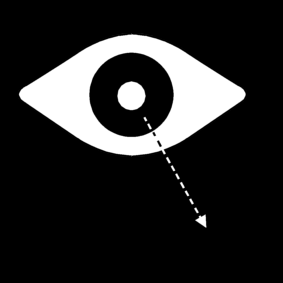
\includegraphics[width=2cm]{sclera/zien}\hspace{0.5cm}}
       {
\includegraphics[width=2cm]{sclera/bus}} \\
       \emph{dog} \emph{see} \emph{bus} \\
    }
    \glt `The dog sees the bus.'
\end{exe}

Ignoring for the time being the missing determiners in
\cref{ex:sclera:dog-see-bus}, it is, so far, possible to conclude that `verb'
pictos can be analysed in much the same way as ordinary verbs with regard to
their valency, despite the fact that, by default, they do not encode for
number, person, tense, aspect or mood, nor are their arguments marked for
number, person or gender (leaving quantification aside for now). Note, too,
that both examples are internally structured according to a
\emph{subject-verb-object} (henceforth \emph{SVO}) element order. Since
\sclera\ is virgin territory as far as its hypothetical syntax is concerned,
there is no evidence to suggest that this is the only word order that a grammar
of \sclera\ should expect, much less that it is the one which ID users would
prefer; however, in the examples that follow, as well as in the grammar model
whose design these examples ultimately inform, \emph{SVO is the word order that
is assumed}\footnote{As discussed later, in \cref{subconc:eval:main}, this is a
serious limitation of the current version of the system. Nevertheless, it is
currently maintained as the only permitted word order because it prevents
structural ambiguity (which arises quickly in the absence of inflection and
other syntactic markings) and allows the analysis of valency and word order to
be implemented relatively easily. Moreover, the combination of multiple
permitted word order patterns in a single grammar represents a complex
undertaking, although, ultimately, it is a goal of the \sclera\ grammar.}.

Structurally, `adjectival' pictographs can also be hypothesized to have
combinatory potential, as examples \cref{ex:sclera:purple-bike} and
\cref{ex:sclera:happy-dog} suggest. Here, \emph{purple} and \emph{happy} can be
seen to modify the `noun' pictos \emph{bike} and \emph{dog}, respectively. Of
course, this is not the only function that such adjectival pictographs can
fill: they can also serve as `nouns' and predicative complements, the latter
function demonstrated in \cref{ex:sclera:dog-is-happy}. (Note that, while
interesting, `adjective' pictos form a minority within the \sclera\ set.
Further, the predicative use of adjectives is not subject to modelling.)

\begin{exe}
    \ex \label{ex:sclera:purple-bike}\attop{
    \gll
       {\includegraphics[width=2cm]{"sclera/kleur paars"}\hspace{0.5cm}}
       {
\includegraphics[width=2cm]{sclera/fiets}}\\
       \emph{purple} \emph{bike}\\
    }
    \glt `The purple bike.'
    %
    \ex \label{ex:sclera:happy-dog}\attop{
    \gll
       {\includegraphics[width=2cm]{"sclera/blij"}\hspace{0.5cm}}
       {
\includegraphics[width=2cm]{sclera/hond1}}\\
       \emph{happy} \emph{dog}\\
    }
    \glt `The happy dog.'
    %
    \ex
    \label{ex:sclera:dog-is-happy}
    *predicative use of adjective picto \\
    \attop{
    \gll
       {\includegraphics[width=2cm]{"sclera/hond1"}\hspace{0.5cm}}
       {
\includegraphics[width=2cm]{sclera/blij}}\\
       \emph{dog} \emph{happy}\\
    }
    \glt `The dog is happy.'
\end{exe}

The foregoing examples all have in common that they involve pictographs
depicting a conceptual simplex: each pictograph corresponds to a single concept
and (in English at least) to single word. However, recall from the inventory of
\sclera\ given in \cref{sub:scleraInventory} that \sclera\ additionally
comprises a large set of pictographs which depict conceptual \emph{complexes}.
These `complex' pictographs generally center on a conceptual process (verb) and
`bundle', as it were, one or more concrete arguments associated with this
process.

There are several kinds of complex pictogaphs. The least problematic for a
traditional constituent-based approach is illustrated in
\cref{ex:sclera:i-go-school}.

\begin{exe}
    \ex\label{ex:sclera:i-go-school}
    \attop{
    \gll
       {
\includegraphics[width=2cm]{sclera/ik}\hspace{0.5cm}}
       {\includegraphics[width=2cm]{"sclera/school gaan 3"}\hspace{0.5cm}}\\
       \emph{I} \emph{go+school} \\
    }
    \glt `I $
        \left\{
            \begin{tabular}{@{}l@{}}
                go \\
                am going
            \end{tabular}
        \right\}
        $ to school.'
\end{exe}

The complex picto in \cref{ex:sclera:i-walk}, \emph{go+school}, depicts two
concepts: a process of `going', and the target of movement, i.e., `school'. In
English (and, incidentally, in Dutch also) the latter is expressed as an
obligatory locative complement, set off by a preposition. Syntactically,
complex pictographs of this kind can be analysed as partially `saturated'
verbal constituents that are still `seeking' an element to fill their subject
slot. Other kinds of complex pictographs, however, may combine with optional
complements, as illustrated by \emph{give+present} in example
\cref{ex:sclera:teacher-give-present}. Such complex pictographs are slightly
less evident, but are generally compatible with SVO phrase structure analyses.

\begin{exe}
    \ex \label{ex:sclera:teacher-give-present}
    \attop{
    \gll
       {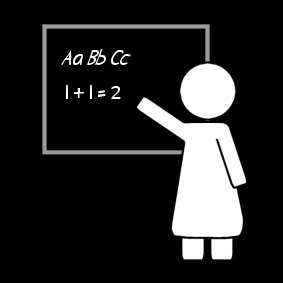
\includegraphics[width=2cm]{sclera/leerkrachte}\hspace{0.5cm}}
       {\includegraphics[width=2cm]{"sclera/geschenkje geven"}\hspace{0.5cm}}
       {\includegraphics[width=2cm]{sclera/jij}} \\
       \emph{teacher} \emph{give+present} \emph{you} \\
    }
    \glt `The teacher gives a present to you.'
\end{exe}

Other pictographs depict conceptual complexes that correspond to entire
clauses, such as \emph{dog+barks} in \cref{ex:sclera:dog-barks}.

\begin{exe}
    \ex \label{ex:sclera:dog-barks}
    \attop{
    \gll
       {\includegraphics[width=2cm]{sclera/hond-blaffen}\hspace{0.5cm}}\\
       \emph{dog+barks}\\
    }
    \glt `The dog barks.'
\end{exe}

Like the absence of determiners/quantifiers, complex pictographs are a feature
of \sclera\ that sets it apart from most `true' natural languages.
Unsurprisingly, therefore, including these pictographs in a grammar model of
\sclera\ requires some slightly different machinery, particularly to make
`constituent' concepts accessible to other parts of the grammar, so that
sequences like in \cref{ex:sclera:happy-dog-barks} are grammatical. We return
to the integration of complex pictographs in \cref{subs:cs:complex-pictos}.
Easier to analyse, simplex pictographs will form the basis of the initial
grammar.

\begin{exe}
    \ex \label{ex:sclera:happy-dog-barks}
    \attop{
    \gll
       {\includegraphics[width=2cm]{sclera/blij}\hspace{0.5cm}}
       {\includegraphics[width=2cm]{sclera/hond-blaffen}\hspace{0.5cm}}\\
       \emph{happy} \emph{dog+barks}\\
    }
    \glt `The happy dog barks.'
\end{exe}

To the best of my knowledge, there currently exist no `corpora' of pictographic
text. The reasons for this are not hard to intuit. Popular and accessible
pictograph-to-text systems are few and far between (hence, the contribution of
this thesis!). If data about how these systems are used collected, it is not
shared. Yet even if it were, pictographic symbol sets vary, making comparison
difficult. As a result of all this, modelling \sclera\ is less a descriptive
than a creative process. Indeed, all the example strings presented in this
sketch are hypothetical, albeit based on linguistic knowledge. As a preface to
the next section, the assumptions which guide this `armchair' approach, as well
as the aims of the forthcoming grammar model, are summarised below.

\paragraph{Grammar aims}

\begin{itemize}
    \item Coverage of simplex picto `(pro)nouns', `verbs', and `adjectives', bearing in mind their underspecified status.
    \item Theory of picto valency/subcategorization patterns
    \item Analysis of missing determiners (\cref{sub:MissingDeterminers}).
    \item Integration of complex pictos.
    \item Ability to parse simple main/matrix clauses and noun phrases
\end{itemize}

\paragraph{Assumptions}

\begin{itemize}
    \item \sclera\ \emph{has} a grammar that can be modelled
    \item The input to the \sclera\ parser consists of lemmas that are
          morpholgically atomic.
    \item The elements on the \sclera\ input adhere to subject-verb-object
          order.
    \item The input can be resolved to a complete main clause or to a
          noun phrase.
\end{itemize}

\subsection{Setting up with the LinGO Matrix}
\label{subs:settingup:lingo}

The starting point for the construction of an implemented grammar of \sclera\
is the \lingo\ Grammar Matrix customization system (introduced in
\cref{ssub:matrixcustomization}). This system, to rephrase its basic function,
generates language-specific extensions of a core type hierarchy, viz., the
\lingo\ Matrix, based on a number of (interactively provided) statements about
properties of the language being modelled.

For ease of prototyping, however, the language that is \emph{actually} modelled
in this step is not \sclera, but the other language with which this thesis
deals, i.e., Dutch (to which we return in the next chapter). This may seem
somewhat confusing at first, particularly at the current level of abstraction,
but the idea is simple and bears mentioning sooner rather than later. As the
observations in the previous section suggest, \sclera\ can (though not
necessarily) be analysed as an SVO language and, as such, shows some
amenability to the mechanisms used in analyses of such languages. Dutch is an
SVO language, too (at least, at certain levels, which I will say more about
later). Thus, one can expect some overlap between \sclera\ and Dutch,
especially on the level of their type hierarchies. Since these grammars are
developed in parallel anyway, from an engineering standpoint, it makes sense to
capitalize on such overlap so that those parts which both grammars have in
common need not be defined twice. Therefore, we opt to use the grammar
customization step to obtain a grammar of Dutch, from which the grammar of
\sclera\ inherits \emph{part} of its type hierarchy. Crudely put, the \sclera\
grammar is an underspecified variant of a model of Dutch (though English would
have worked just as well) with a few \sclera-specific additions, which are
introduced in the following sections. However, this does not mean that the
\sclera\ grammar will be indefinitely tethered to the grammar of Dutch: it is a
marriage of convenience, not necessity. Eventually, the two will be untangled
into two discrete grammars. For reference purposes,
\cref{ex:table:scleraComponents} shows how the \sclera\ grammar's components
are related with respect to the names of the associated files.

\begin{exe}
    \ex\label{ex:table:scleraComponents}\attop{
    \small
    \begin{tabular}[h]{ p{5.4cm} | p{5.9cm} }
        \hline
        \textbf{Exclusive to \sclera} & \textbf{Inherited from Dutch grammar} \\
        \hline
        \texttt{mini-sclera.tdl}\newline(\sclera-specific type hierarchy; Developed in sections \ref{sub:MissingDeterminers} and \ref{sec:casestudies}) & \texttt{matrix.tdl}\newline(\lingo\ Matrix core type hierarchy ($\pm$ 3800 lines)) \\
        \texttt{lexicon.tdl}\newline(contains lexical entries for pictograph identifiers) & \texttt{mini-dutch.tdl} \newline (type hierarchy of Dutch) \\
        \texttt{rules.tdl}\newline(contains phrase rule entries) & \texttt{head-types.tdl} \newline(recent addition to Matrix (not discussed); defines disjunctive head types) \\
        \texttt{lrules.tdl}\newline(contains lexical rule entries) & \texttt{roots.tdl}\newline(list of structures which can serve as start symbol) \\
        \texttt{config.tdl}\newline(Initial configuration file used by \ace\ during compilation; concerns settings) & \texttt{labels.tdl} \newline(specifies labels for nodes in syntax trees (forwhen using visual modes)) \\
        \texttt{mini-sclera-top.tdl}\newline(Second \ace\ configuration file; points compiler to appropriate files) & \texttt{semi.vpm}\newline(Virtual Property Mapping interface (Not introduced in \cref{ssub:delphinstructure} on account of its rather technical nature; mediates between `internal' and `external' \mrs\ representations; see the \delphin\ wiki entry at  \href{http://moin.delph-in.net/RmrsVpm}{\texttt{moin.delph-in.net/RmrsVpm}})) \\
        \hline
    \end{tabular}
    }
\end{exe}

To recapitulate, the result of the customization step is \emph{actually} an
initial grammar of Dutch, from which an initial grammar of \sclera\ is derived.
Although the two grammars bifurcate slightly as they are extended later on
(large parts of either are, in fact, later re-written or replaced with patches
from other \delphin\ grammars), at this stage, the grammar of \sclera\ can be
thought of simply as a less specific, i.e., more `permissive', variant of the
grammar of Dutch. The grammar inherits all of the other's type constraints, but
leaves these underspecified where necessary, for instance, when a given feature
is not relevant.

The primary locus of underspecification is the lexicon. To illustrate this,
compare the lexical entry for \emph{hond} (`dog') in the grammar of Dutch
\cref{ex:Dutch:hond}) to the lexical entry for the picto \emph{dog} in the
grammar of sclera \cref{ex:Sclera:dog2}. (Note that the pictograph
identifier, specified on the list value of the \textsc{stem} attribute, is provided as a simple lemma, as discussed in \cref{sec:picto-identifiers}.)

\begin{exe}
    % \label{}
    \ex\label{ex:Dutch:hond} Lexical entry for Dutch \emph{hond} (`dog')\\
    \small
    \begin{verbatim}
hond := femmasc-count-sg-noun-lex &
  [ STEM < "hond" >,
    SYNSEM.LKEYS.KEYREL.PRED "_hond_n_rel" ].
    \end{verbatim}
    \ex\label{ex:Sclera:dog2} Lexical entry for picto depicting `dog'\\
    \small
    \begin{verbatim}
dog := common-noun-lex &
  [ STEM < "dog" >,
    SYNSEM.LKEYS.KEYREL.PRED "_dog_n_rel" ].
    \end{verbatim}
\end{exe}

The types with which these lexical entries are identified, viz.,
\emph{femmasc-count-sg-noun-lex} and \emph{common-noun-lex}, are situated on
different levels of the type hierarchy. As the local hierarchy in
\cref{ex:scleragram:typeh:nouns} shows, \emph{common-noun-lex} is a supertype
of \emph{femmasc-count-sg-noun-lex}. It inherits from \emph{obl-spr-noun-lex}
itself, which in turn multiply inherits from several other general types. (The
dashed edges between tree nodes indicate where the hierarchy has been
purposefully simplified.) Lexical entries of the type \emph{common-noun-lex},
an AVM example of which is given in \cref{ex:sclera:common-noun}, have a
\textsc{head} attribute that takes values of the type \emph{noun} (which can be
specified for the feature \textsc{case}), require one \emph{obligatory}
argument\footnote{See \cref{sub:MissingDeterminers}}, which is identified with
the value of the SPecifieR (\textsc{spr}) attribute (used to build
determiner/quantifier-noun phrases), and, on a semantic level, have additional
appropriate features \emph{person}, \emph{number}, and \emph{gender}, which
correspond to \mrs\ variables, but \emph{common-noun-lex} does not stipulate
any constraints on the values of these \mrs\ variables. As a result, the
lexical entry for the pictograph `dog' is appropriately identified with the
part-of-speech category `noun', but is left entirely underspecified with
respect to the features number, person and (since this varies from language to
language) gender. By contrast, the types used in the lexicon of the grammar of
Dutch are more specific. For instance, by inheriting from
\emph{femmasc-count-sg-noun-lex}, the lexical entry in \cref{ex:Dutch:hond} is
defined explicitly as being singular, non-neuter (feminine or masculine), and
count (requiring an explicit determiner). This is appropriate because these
features are relevant to the syntax of Dutch.

\begin{exe}
    \ex\label{ex:sclera:common-noun}
    \vspace{0.5cm}
    \begin{avm}
        [ \asort{common-noun-lex}
          stem \; < \avmstring{dog} > \\
          synsem|local & [ cat & [ head \; [ \asort{noun}
                                             case & case \\
                                             mod & \<\;\> ] \\
                                 val [subj & \<\;\> \\
                                      spr & \< @1
                                        [ local|cat|head & det \\
                                          opt \; \textnormal{-}  ] \> \\
                                          comps & \<\;\> ] ] \\
                           cont & [ hook|index|png\;[ \asort{ref-ind}
                                                      per & person \\
                                                      num & number \\
                                                      gend & gender ] \\
                                  rels \; < [
                                         \asort{ep}
                                          pred & \avmstring{\_dog\_n\_rel} ] >\\
                                   hcons \; \<\;\> ]  ] \\
          arg-st \; \< @1 \>  ]
    \end{avm}
\end{exe}

\begin{exe}
    \ex\label{ex:scleragram:typeh:nouns}\attop{
    \tikzset{every tree node/.style={anchor=base}}
    \begin{tikzpicture}
        \Tree  [.\texttt{lex-item} \edge[dashed];
               [.\texttt{basic-noun-lex} \edge[dashed];
               [.\texttt{noun-lex} \edge[dashed];
               [.\texttt{obl-spr-noun-lex}
               [. \node[draw] {\texttt{common-noun-lex}};
               \edge[thick];
               [. \node[draw] {\texttt{femmasc-count-sg-noun-lex}}; ]
               \edge[dashed];
               [.\texttt{femmasc-count-pl-noun-lex} ] ] ] ] ] ]
                % ]
    \end{tikzpicture}
    } % attop
\end{exe}

`Verb' pictographs in the lexicon of the \sclera\ grammar are similarly
identified with comparatively general lexical types. As may be intuited
partially from the associated type names, the constraints for which entries in
the Dutch grammar are specified (including \emph{person}, \emph{number}, and
\emph{tense}) are left underspecified in equivalent entries in the grammar of
\sclera. Once again, an illustration of the (local) type hierarchy, given in
\cref{ex:scleragram:typeh:intrans}, does much in the way of clarity.

\begin{exe}
    % \label{}
    \ex\label{ex:dutch:slaapt}
        \small
        \begin{verbatim}
slaapt := intrans-2nd-or-3rd-sg-verb-lex &
  [ STEM < "slaapt" >,
    SYNSEM.LKEYS.KEYREL.PRED "_slapen_v_rel" ].
        \end{verbatim}
    \ex\label{ex:sclera:sleep}
    \small
    \begin{verbatim}
sleep := intrans-verb-lex &
  [ STEM < "sleep" >,
    SYNSEM.LKEYS.KEYREL.PRED "_sleep_v_rel" ].
    \end{verbatim}
\end{exe}

\begin{exe}
    \ex\label{ex:scleragram:typeh:intrans}\attop{
    \tikzset{every tree node/.style={anchor=base}}
    \begin{tikzpicture}
        \Tree  [.\texttt{lex-item} \edge[dashed];
               [.\texttt{verb-lex} \edge[dashed];
               [.\texttt{main-verb-lex};
                  [.\texttt{intransitive-verb-lex}
                    [.\texttt{nom-intransitive-verb-lex}
                    [. \node[draw] {\texttt{intrans-verb-lex}};
                    %   \edge[thick];
                    [. \node[draw] {\texttt{intrans-2nd-or-3rd-sg-verb-lex}}; ] ] ] ] ]
                \edge[dashed];
                [.\texttt{transitive-verb-lex} ] ] ]
                % ]
    \end{tikzpicture}
    } % attop
\end{exe}

Turning now to phrase structure rules -- at this stage, the grammar of \sclera\
uses the same basic rule types as defined by the grammar of Dutch. The three
most important correspond to the `schemata' of canonical \hpsg
\citep{pollard1994head}. Provided as entries in \texttt{rules.tdl}, as shown in
\cref{ex:sclera:rulestdl}, these types instantiate the backbone for the SVO
order assumed of \sclera\ strings in the previous section.

\begin{exe}

    \ex\label{ex:sclera:rulestdl}Top of \texttt{rules.tdl}\\
    \begin{verbatim}
head-comp := head-comp-phrase. ;; (1)
subj-head := subj-head-phrase. ;; (2)
head-spec := head-spec-phrase. ;; (3)
    \end{verbatim}
\end{exe}

Word order is accounted for by combining rule types that impart unique
`headedness' to the daughters of a phrase with rules that constrain the linear
position of the head daughter in relation to her non-head sisters. For
instance, the \emph{head-complement phrase} rule, in
\cref{ex:sclera:rule:headcomp}, combines the constraints of
\emph{basic-head-1st-comp-phrase} (a subtype of `dominance' rule types
involving complements) with the constraints belonging to the type
\emph{head-initial}, which, as its name suggests, requires that the head
daughter come first in the phrase. Variations on this logic are used in the
type definitions of the other two rules, except here the head daughter is
required, by \emph{head-final}, to come last, or -- as these rules are
consistently binary (see \cref{par:naryvsbinary}) -- second.

\begin{exe}
    \ex\label{ex:sclera:rule:headcomp}
\begin{verbatim}
head-comp-phrase := basic-head-1st-comp-phrase & head-initial.
\end{verbatim}
    \ex\label{ex:sclera:rule:subjhead}
\begin{verbatim}
subj-head-phrase := decl-head-subj-phrase & head-final &
    [ HEAD-DTR.SYNSEM.LOCAL.CAT.VAL.COMPS < > ].
\end{verbatim}
    \ex\label{ex:sclera:rule:headspec}
\begin{verbatim}
head-spec-phrase := basic-head-spec-phrase & head-final.
\end{verbatim}
\end{exe}

The result of the customization stage (followed by a fair amount of manual
intervention) is a partial model of \sclera\ comprising, among other, type
descriptions for simplex `noun' and `verb' pictographs and basic grammar rules
for phrase construction (which, it ought to be mentioned, also implement the
semantic composition principles of \hpsg\ \citep{sag1999syntactic}) as well as
the internal structure of phrases, with respect to both linear precedence and
immediate dominance \citep{pollard1994head}. However, the current model is not
entirely ready to be used for parsing yet. The next section aims to fix this.

\subsection{`Bringing back' determiners}
\label{sub:MissingDeterminers}

Recall that the function of the grammar of \sclera\ within the \depicto\ system
is to `extract' as much semantic information as possible from the pictographic
input, which, by natural language standards, is vastly underspecified. In order
to do this, then, the grammar must be able to make hypotheses about semantic
structure based on what little clues the input affords. The grammar developed
so far does not do this, however; only the immediate surface structure of the
input is taken into account. As a result, the absence of determiners in the
\sclera\ language causes the grammar to run into trouble. This is because of
two reasons. First, on a theoretical level, the \lingo\ Matrix incorporates the
assumption that the referential indices, i.e., `noun' predications, of a
well-formed \mrs\ must always be outscoped by some quantifier
\citep{copestake2005minimal}. Second, in the grammar of Dutch, from which the
grammar of \sclera\ derives its types, this assumption is worked out by an
interplay of constraints which have the effect of requiring that common nouns
select for an obligatory `specifier' (quantifier/determiner). This is what is
specified by the negative value of the \textsc{opt} attribute in the AVM
description of the type \emph{common-noun-lex} in \cref{ex:sclera:common-noun},
the relevant portion of which is repeated here in
\cref{ex:sclera:featurepath:opt-}. Since determiners do not occur on the input,
the parser fails when passed a \sclera\ string containing pictographs of the
`common noun' type.

\begin{exe}
    \ex\label{ex:sclera:featurepath:opt-}
    \begin{avm}
        [ \asort{common-noun-lex}
           synsem|local|cat|cal|spr &  < [ local|cat|head & det \\
                                        opt \; \textnormal{-} ] > ]
    \end{avm}
\end{exe}

However, not all types of nouns select an explicit determiner, as
\cref{ex:mass-noun} and \cref{ex-pronoun} show for mass nouns and pronouns,
respectively. These types take either no specifier or take one but mark it as
optional.

\begin{exe}
    \ex\label{ex:mass-noun}
            \textbf{Water} has three forms.
    \ex\label{ex-pronoun}
            \textbf{You} should tell \textbf{me} about \textbf{them}.
\end{exe}

When occurring without a specifier, as in the examples above, these noun types
form so-called \emph{bare noun phrases}. However, semantically, their
referential indices are still scoped by an `exist' quantifier, as represented
semi-formally in \cref{ex:exist-noun}.

\begin{exe}
    \ex\label{ex:exist-noun}
    $ exists(x, noun\_relation(x) )$
\end{exe}

In order to achieve this effect, the \lingo\ Matrix provides a definition of a
unary phrase rule type that takes a single nominal head daughter with an
optional specifier constraint and \emph{adds} a quantification relation to the
list of \emph{elementary predications} provided by the head daughter. The
semantic contribution of the rule is specified on the attribute \textsc{c-cont}
(\emph{Construction CONTent}). As the identity statements (prefixed by a
`\textsc{\#}') in the \tdl\ description in \cref{ex:dutch:bare-np-phrase:verb}
show, the \textsc{c-cont} part of the rule identifies the daughter's
\emph{index} with the index argument (\textsc{arg0}) of \emph{quant-relation}.
At the same time time, via identity with an attribute of the handle constraint
relation in \textsc{hcons}, the top handle (\textsc{ltop}) of the daughter is
placed within the quantifier's scope.

\begin{exe}
    \ex\label{ex:dutch:bare-np-phrase:verb}
    {\small
    \begin{verbatim}
basic-bare-np-phrase := head-only &
  [ SYNSEM.LOCAL.CAT.VAL [ SPR < >,
               SUBJ < >,
               COMPS < >,
               SPEC < > ],
    HEAD-DTR.SYNSEM.LOCAL [ CAT [ HEAD noun,
                                  VAL [ SPR < [ LOCAL.CAT.HEAD det,
                                                OPT + ] >,
                                        SUBJ < >,
                                        COMPS < > ] ],
                            CONT.HOOK [ INDEX #index,
                                        LTOP #larg ] ],
    C-CONT [ RELS <! quant-relation &
                        [ ARG0 #index,
                          RSTR #harg ] !>,
             HCONS <! qeq &
                       [ HARG #harg,
                         LARG #larg ] !>,
             ICONS <! !>,
             HOOK [ INDEX #index ] ] ].
    \end{verbatim}
    }
\end{exe}

The Matrix definition of the rule leaves the specification of the quantifier's
\textsc{pred} value (i.e., relation name) to the precise grammar in which it is
used. In the grammar of \sclera\ this becomes \emph{`exist\_q\_rel'}, as shown in \cref{ex:sclera:bare-np:verb}.

\begin{exe}
    \ex\label{ex:sclera:bare-np:verb}
    {\small
    \begin{verbatim}
bare-np-phrase := basic-bare-np-phrase &
  [ C-CONT.RELS <! [ PRED 'exist_q_rel' ]  !> ].
    \end{verbatim}
    }
\end{exe}

Example \cref{ex:sclera:bare-np:tree} shows the \emph{basic-np-phrase} rule
being used to parse the mass noun \emph{water} (as it is used
\cref{ex:mass-noun}). Notice that the mother node, i.e., the value of the
top-level feature path \textsc{synsem|local}, is (a) a saturated noun phrase
(NP), which makes the resulting structure compatible with the head-complement
and head-subject rules; and (b) that its relations list (under \textsc{cont})
is the append of those of \textsc{c-cont} and \textsc{head-dtr}. In short, the
semantic content of the mother node, or, as it were, the `left side' of the
phrase rule, contains \emph{more} than what is found on the actual input.

\begin{exe}
    \ex\label{ex:sclera:bare-np:tree}
    \avmoptions{notactive}
    \tikzset{every tree node/.style={align=center,anchor=north}}
    \tikzset{level 1/.style={level distance=320pt}}
    \tikzset{level 2/.style={level distance=180pt}}
    \attop{\begin{tikzpicture}
    % [level distance=250pt]
\Tree [ .NP\\{
    \begin{avm}
\[ \asort{bare-np-phrase}
   synsem\|local & \[ cat\|val\|spr \; <\;> \\
                      cont \; \[ hook\|index \; \@2  \\
                                 rels  \; \@5 $\oplus$ \@4 \]  \] \\
   c-cont & \[ hook\|index \; \@2 \\
               rels \; \@5 \< \[ pred & \avmstring{exist\_q\_rel} \\
                                 arg0 & \@2  \\
                                 rstr & \@6 \]  \>  \\
               hcons \; \< \[ \asort{qeq}
                              harg & \@6 \\
                              larg & \@3 \] \> \] \\
   head-dtr \; \@1 \]
     \end{avm} }
        [ .N\\{
\begin{avm}
\@1 \[ synsem\|local & \[ cat\|val\|spr \; \< \[ local\|cat\|head & det \\
                                            opt \; \textnormal{+} \] \> \\
                         cont \; \[ hook & \[ index & \@2 \\
                                             ltop & \@3 \] \\
                                   rels & \@4 \< \[ pred &
                                            \avmstring{\_water\_n\_rel}  \]
                                               \> \] \] \]
\end{avm} }
           water ] ]
        \end{tikzpicture}
        } % attop
\end{exe}

This notion that a phrase rule can itself \emph{contribute} semantic
information (or simply modify it) forms the basis for many of the analyses
which enable the \sclera\ grammar to make the best of its semantically
impoverished input, including the grammar's treatment of missing determiners.
(In fact, if the foregoing explanation is at all clear, the reader may by now
already have some idea as to how this might work.) All that is needed to `bring
back' determiners is a slightly modified version of the \emph{bare-np-phrase}
rule which unifies with common nouns, i.e., noun entries with a
\emph{non-optional} specifier constraint, and places these nouns in a similar
scoping relation. The \emph{bare-np-phrase} rule, therefore, is copied and
modified accordingly to obtain the \tdl\ description in
\cref{ex:sclera:sclera-basic-insert-det-rule:verb}. Notice that, instead of
`exist\_q\_rel', this rule contributes a new quantifier relation,
`q\_rel\_min'. Though specified as a string in the \sclera\ grammar, this
quantifier relation is later converted to a type, which, as the next chapter
will explain in more detail, is situated at the top of a local hierarchy of
different determiner and quantifier relations. Slightly ahead of time (the
hierarchy is the domain of the target grammar), this hierarchy of determiner
types is shown in \cref{ex:dutch-sclera:quantifier-types:tree}). By virtue of
the \emph{sclera-basic-insert-det} rule, the \sclera\ grammar can now parse
strings containing common nouns without requiring that these be accompanied by
(non-existent) determiners.


\begin{exe}
    \ex\label{ex:sclera:sclera-basic-insert-det-rule:verb}
    {\small
    \begin{verbatim}
sclera-basic-insert-det-rule := head-only &
  [ SYNSEM.LOCAL.CAT.VAL [ SPR < >,
                           SUBJ < >,
                           COMPS < >,
                           SPEC < > ],
    HEAD-DTR.SYNSEM.LOCAL [ CAT [ HEAD noun,
                                  VAL [ SPR < [ LOCAL.CAT.HEAD det,
                                                OPT - ] >,
                                        SUBJ < >,
                                        COMPS < > ] ],
                            CONT.HOOK [ INDEX #index,
                                        LTOP #larg ] ],
    C-CONT [ RELS <! quant-relation &
                      [ PRED "q_rel_min",
                        ARG0 #index,
                        RSTR #harg ] !>,
             HCONS <! qeq &
                      [ HARG #harg,
                        LARG #larg ] !>,
             ICONS <! !>,
             HOOK [ INDEX #index,
                    LTOP #larg ] ] ].
    \end{verbatim}
    }
\end{exe}


\begin{exe}
    \ex\label{ex:dutch-sclera:quantifier-types:tree}
    \tikzset{every tree node/.style={align=center,anchor=north}}
    \attop{
    \emph{
    \begin{tikzpicture}
        \Tree [.predsort
                [.q\_rel\_min
                   def\_q\_rel\\{\textnormal{(definite determiner)}}
                   indef\_q\_rel\\{\textnormal{(indefinite determiner)}}
                   exist\_q\_rel\\{\textnormal{(`exists' relation)}} ] ]
    \end{tikzpicture}
    } % emph
    } % attop
\end{exe}

The parse of \sclera\ `dog', represented as a tree diagram in
\cref{ex:sclera:insert-det-rule:tree}, is clearly similar to that licensed by
the rule upon which it is based. In fact, the differences are hard to spot. Yet
the importance of the \emph{sclera-insert-det-rule} for the grammar of \sclera\
cannot be overstated.

\begin{exe}
    \ex\label{ex:sclera:insert-det-rule:tree}
    \avmoptions{notactive}
    \tikzset{every tree node/.style={align=center,anchor=north}}
    \tikzset{level 1/.style={level distance=320pt}}
    \tikzset{level 2/.style={level distance=180pt}}
    \attop{\begin{tikzpicture}
    % [level distance=250pt]
\Tree [ .NP\\{
    \begin{avm}
\[ \asort{sclera-basic-insert-det-rule}
   synsem\|local & \[ cat\|val\|spr \; <\;> \\
                      cont \; \[ hook\|index \; \@2  \\
                                 rels  \; \@5 $\oplus$ \@4 \]  \] \\
   c-cont & \[ hook\|index \; \@2 \\
               rels \; \@5 \< \[ pred & \avmstring{q\_rel\_min} \\
                                 arg0 & \@2  \\
                                 rstr & \@6 \]  \>  \\
               hcons \; \< \[ \asort{qeq}
                              harg & \@6 \\
                              larg & \@3 \] \> \] \\
   head-dtr \; \@1 \]
     \end{avm} }
        [ .N\\{
\begin{avm}
\@1 \[ synsem\|local & \[ cat\|val\|spr \; \< \[ local\|cat\|head & det \\
                                            opt \; \textnormal{-} \] \> \\
                         cont \; \[ hook & \[ index & \@2 \\
                                             ltop & \@3 \] \\
                                   rels & \@4 \< \[ pred &
                                            \avmstring{\_dog\_n\_rel}  \]
                                               \> \] \] \]
\end{avm} }
           \includegraphics[width=2cm]{sclera/hond1} ] ]
        \end{tikzpicture}
        } % attop
\end{exe}

With the \emph{sclera-insert-det-rule} in place, the grammar can now parse
simple \sclera\ strings of the kind shown in \cref{ex:sclera:dog-see-bus},
repeated for convenience here by \cref{ex:sclera:dog-see-bus1}. The tree
diagram representation of the parse is given in
\cref{ex:sclera:dog-see-bus:tree}.

\begin{exe}
    \ex \label{ex:sclera:dog-see-bus1}\attop{
    \gll
       {\includegraphics[width=2cm]{sclera/hond3}\hspace{0.5cm}}
       {\includegraphics[width=2cm]{sclera/zien}\hspace{0.5cm}}
       {\includegraphics[width=2cm]{sclera/bus}} \\
       \emph{dog} \emph{see} \emph{bus} \\
    }
\end{exe}


\begin{exe}
    \ex\label{ex:sclera:dog-see-bus:tree}
    \tikzset{every tree node/.style={align=center,anchor=north}}
        \tikzset{level 3/.style={level distance=30pt}}
    \attop{
    \begin{tikzpicture}[level distance=50pt]
        \Tree [.S\\{\emph{head-subject rule}}
                   [.NP\\{\emph{sclera-det-insert rule}}
                       [.N {`dog'} ] ]
                   [.VP\\{\emph{head-complement rule}} [ .V {`see'} ]
                    .NP\\{\emph{sclera-det-insert rule}} [ .N {`bus'} ] ] ]
    \end{tikzpicture}
    }
\end{exe}

\section{Understanding the \mrs\ output}
\label{sec:sclera:mrsoutput}

When using the \ace\ processor \citep{sweaglesACE}, the output of parsing is a
\emph{plain-text} \mrs\ representation. An example of such an \mrs\
representation is given in \cref{ex:sclera:outputofparsing:text}, which shows
the fully semantic structure to which the string in
\cref{ex:sclera:dog-see-bus:tree} resolves, i.e., the semantic information
found at the root node `S'.

\begin{exe}
    \ex\label{ex:sclera:outputofparsing:text} Output \mrs\ representation of `dog see bus'\\
    \scriptsize
    \begin{verbatim}
SENT: dog see bus
[ LTOP: h0
  INDEX: e2 [ e SF: prop-or-ques E.TENSE: tense E.ASPECT: aspect E.MOOD: mood ]
  RELS: < [ "_dog_n_rel"<-1:-1> LBL: h4 ARG0: x3 [ x PNG.PER: person
                                                     PNG.NUM: number
                                                     PNG.GEND: gender ] ]
          [ "q_rel_min"<-1:-1> LBL: h5 ARG0: x3 RSTR: h6 BODY: h7 ]
          [ "_see_v_rel"<-1:-1> LBL: h1 ARG0: e2 ARG1: x3 ARG2: x8 [ x PNG.PER: person
                                                                       PNG.NUM: number
                                                                       PNG.GEND: gender ] ]
          [ "_bus_n_rel"<-1:-1> LBL: h9 ARG0: x8 ]
          [ "q_rel_min"<-1:-1> LBL: h10 ARG0: x8 RSTR: h11 BODY: h12 ] >
  HCONS: < h0 qeq h1 h6 qeq h4 h11 qeq h9 > ]
    \end{verbatim}
\end{exe}

Although the representation in the example has been slightly simplified (and
beautified with extra indentation), it may be observed that its general format
approximates that of the AVM diagram given in \cref{sub:mrs}. However, there
are also some differences. The attributes \textsc{ltop} and \textsc{index} are
taken out of the \textsc{hook} feature and promoted to the top level of the
representation, and, presumably for legibility, the \emph{qeq} constraints are
not presented as individual feature structures, nor are they separated by a
comma. More salient, however, is the appearance of attribute-value pairs such
as \texttt{E.TENSE: tense} and \texttt{PNG.GEND: gender} after referential
variables (e.g., \texttt{x8}) and event variables (e.g., \texttt{e2}). These
convey additional semantic properties associated with the values of the
attributes \textsc{index} or \textsc{arg0}. In example
\cref{ex:sclera:outputofparsing:text}, all but one are left underspecified: the
value of \texttt{SF} (third line from the top) conveys that the illocutionary
force of the parsed string is either declarative or interrogative. When the
parsed string contains pronouns, however, the properties of the referential
index/variable are more specific, as the fragment in \cref{ex:sclera:outputofparsing:I} shows. The referential (`\texttt{ARG0}') argument of the predicate `\_pronoun\_n\_rel' has the property of being first person singular (\emph{I} in English), but leaves the value of the \texttt{GEND} property underspecified, since it is gender-neutral.

\begin{exe}
    \ex\label{ex:sclera:outputofparsing:I} Fragment of \mrs\ representation of `I walk'\\
    \scriptsize
    \begin{verbatim}
RELS: < [ "_pronoun_n_rel"<-1:-1> LBL: h4 ARG0: x3 [ x PNG.PER: 1st
                                                       PNG.NUM: singular
                                                       PNG.GEND: gender ] ]
    \end{verbatim}
\end{exe}

\section{Extending the \sclera\ grammar}
\label{sec:casestudies}

This section presents three case studies which extend the grammar of \sclera\
developed in the previous section and, in so doing, offer some indication,
albeit tentative, of the practicability of a rule-based approach to modelling
\sclera\ as a language in its own right. \cref{subs:cs:temp-disambig} and
\cref{subs:cs:interrogative} introduce two new phrase rules that demonstrate
how the semantic accuracy of the grammar can be enhanced so that it can
distinguish, on the one hand, between past and `other' tense readings of the
input and, on the other hand, between declarative and illocutionary readings.
Abstractly, both phrase rules function by identifying a specific non-head
daughter `particle' and modifying the semantic content of the head daughter to
match some feature contributed by this `particle'. (Such particles can also be
thought of as `indicators' or `operators'. In part-of-speech terms, they
correspond to adverbs, though there are some differences in overall function.)
Moving on, the third case study (\cref{subs:cs:complex-pictos}) details a first
attempt at extending the grammar's coverage to conceptually complex
pictographs. I say `first attempt' because (a) only a selection of complex
pictograph types has so far been incorporated; (b) the local type hierarchy
which they deploy is fairly rudimentary; and (c) as a result, the division of
labor between the lexicon and the type hierarchy is currently biased toward the
lexicon. Nevertheless, the discussion in this section demonstrates that complex
pictographs \emph{can} in principle be incorporated, provided that a handful of
new rules and two new additions to the feature geometry are introduced.

\subsection{Temporal disambiguation} %  with adverbial pictos
\label{subs:cs:temp-disambig}

\sclera\ `verbs' are underspecified for tense. As a result, the clause
structures which they project allow as many readings as there are tenses
available in the semantic universe. Thus, supposing a minimal theory of tense
types, the string in \cref{ex:sclera:dog-see-bus1} can correspond, among other,
to the three different readings shown in \cref{ex:temp:readingsbasic1}, all
other sources of underspecification kept equal.

\begin{exe}
    \ex\label{ex:temp:readingsbasic1} `dog see bus' $ \Leftrightarrow $
    \begin{xlist}
        \ex `The dog \emph{sees} the bus.' (Present tense domain)
        \ex `The dog \emph{saw} the bus.' (Past tense domain)
        \ex `The dog \emph{will} see the bus.' (Future tense domain )
    \end{xlist}
\end{exe}

Similar to the `re-introduced' determiner relation in
\cref{sub:MissingDeterminers}, which, as we saw there, is actually a
generalization over several concrete kinds of determiners, the \emph{intended}
tense of a simple string such as `dog see bus' is grammatically undecidable,
and is therefore best left underspecified. It is arguably a limitation of the
\sclera\ set that it does not contain pictographs which explicitly specify the
intended tense. However, the set does contain a number of pictographs that
depict temporal concepts and which can conceivably function as adjuncts of time
in a \sclera\ clause. A selection is given by \cref{ex:temp:pictosoftime}.

\begin{exe}
    \ex
    \label{ex:temp:pictosoftime}
    \attop{
    \gll
    {\includegraphics[height=2cm]{sclera/gisteren}\hspace{0.2cm}}
    {\includegraphics[height=2cm]{sclera/vandaag}\hspace{0.2cm}}
    {\includegraphics[height=2cm]{sclera/nu}\hspace{0.2cm}}
    {\includegraphics[height=2cm]{sclera/morgen}}\\
    {`yesterday'} {`today'} {`now'} {`tomorrow'}\\
    } % attop
\end{exe}

In natural language, such time adjuncts are generally appropriate to a single
specific temporal domain. As \cref{ex:temp:read/w/yest} illustrates for
`yesterday', the effect in \sclera\ is that they restrict the felicitousness of
individual tense readings.

\begin{exe}
    \ex\label{ex:temp:read/w/yest} `dog see bus yesterday'
        $ \Leftrightarrow $
    \begin{xlist}
        \ex[]{`The dog \emph{saw} the bus yesterday.'}
        \ex[*]{`The dog \emph{sees} the bus yesterday.'}
        \ex[*]{`The dog \emph{will} see the bius yesterday.'}
    \end{xlist}
\end{exe}

From a procedural perspective, these adjuncts can be understood as
\emph{modifying} the tense of the verb phrase with which they combine so that
its tense is constrained to a specific type. This behavior is modelled by the
introduction of a new phrase rule type called
\textbf{\emph{temp-adverb-verb-phrase}} (the adjuncts of time in
\cref{ex:temp:pictosoftime} are analysed as simple adverbs here). As its \tdl\
description shows, this rule belongs to the `head-modifier' category
\citep{pollard1994head}. Essentially, it identifies the \textsc{tense} value of
the index of its non-head daughter, which must be an adverb\footnote{In \hpsg,
adverbs are treated semantically as `events' \citep{pollard1994head}}, with the
\textsc{tense} value of the index of \textsc{c-cont}. The index of this last
feature is passed up to the mother of the rule through constraints inherited
from its supertypes. While \textsc{c-cont} shares its \textsc{tense} value with
the adverbial daughter, all features found under \textsc{c-cont}'s
\textsc{hook} attribute are shared with those of the head daughter, including
the \textsc{tense} attribute. By virtue of unification, however, the compatible
yet more specific value of the non-head daughter's \textsc{tense} feature
`wins', as it were, over the more general value of the head-daughter's
\textsc{tense} feature. For the time being, finally, the rule requires the head
daughter to be a finite clause, specified by \texttt{[ CAT.MC + ]}. This goes
against conventional wisdom, which analyzes adjuncts as modifying the verb
phrase, not the clause as a whole, and should probably be revised later on.

\begin{exe}
    \ex\label{ex:temp:temp-phrase:verb}
    {\small
    \begin{verbatim}
temp-adverb-verb-phrase := basic-head-mod-phrase-simple &
                                head-initial & isect-mod-phrase &
  [ C-CONT.HOOK #hook & [ INDEX.E.TENSE #tense ],
    NON-HEAD-DTR.SYNSEM.LOCAL [ CAT.HEAD adv,
                                CONT.HOOK.INDEX.E.TENSE #tense ],
    HEAD-DTR.SYNSEM.LOCAL [ CONT.HOOK #hook,
                            CAT.MC + ] ].
    \end{verbatim}
    }
\end{exe}

As the tree representation of the parse of the string `dog see bus
yesterday' in \cref{ex:temp:temp-adv-verb:tree} shows, the effect of the
\emph{temp-adverb-verb-phrase} rule is that the adjunct of time `imparts' its
\textsc{tense} constraint to the clause/verb phrase which it modifies.

\begin{exe}
    \ex\label{ex:temp:temp-adv-verb:tree}
    \avmoptions{notactive}
    \avmhskip{0.5em}
    \tikzset{every tree node/.style={align=center,anchor=base}}
    \tikzset{level 1/.style={level distance=160pt}}
    \tikzset{level 2/.style={level distance=120pt}}
    % \tikzset{level 3/.style={level distance=40pt}}
    \attop{
    \noindent
    \begin{tikzpicture}
    % [level distance=250pt]
\Tree [ .S\\{
    \begin{avm}
\[ \asort{temp-adverb-verb-phrase}
   synsem\|local & \[ cat\|head & verb \\
                      cont\|hook & \@1 \] \\
   c-cont\|hook & \@1 \[ index\|e\|tense & \@3 \] \\
   head-dtr & \@2 \\
   non-head-dtr & \@4 \]
    \end{avm}}
          [ .S\\{
          \begin{avm}
\@2 \[ cat \; \[ head & verb \\
                mc & \textnormal{+} \] \\
       cont\|hook \; \@1 \[ index\|e\|tense & tense \] \]
          \end{avm}}
                \edge[roof]; {`dog see bus'} ]  % left ]
          [ .Adv\\{  % right
                \begin{avm}
\@4 \[ \asort{temporal-adjunct-picto}
       cat\|head \; \[ \asort{adverb}
                  mod & \< \@2 \> \]  \\
          cont\|hook\|index\|e\|tense & \@3 past \]
                \end{avm}}
                `yesterday' ] ]
        \end{tikzpicture}
        } % attop
\end{exe}

Just like the rule responsible for the `re-introduction' of determiners, the
\emph{temp-adverb-verb-phrase} rule offers a means of enriching the semantic
structure that is extracted from the input string during parsing. Later on in
the translation process (in the generation stage, to be specific), the
resulting increase in specificity will amount to increased accuracy. Itself
still a proof of concept, the rule is not as `strict' as it should be: it is
not constrained to time adjuncts \emph{only}. However, since the grammar
currently models only one adverb and this adverb is the time adjunct
`yesterday', this does not pose any problems at the moment. To be clear,
however, adding the remaining time adjunct pictos listed in
\cref{ex:temp:pictosoftime} to the grammar would be a relatively simple task.

Finally, the \emph{temp-adverb-verb-phrase} rule exhibits two limitations that
will need to be overcome if it is to be useful in a real-life context. The
first is that the head daughter is required to come \emph{before} the modifying
daughter and that this head daughter needs to be a finite clause. Ignoring the
second issue, the restriction on word order prevents even simple variations on
the string in \cref{ex:temp:read/w/yest} from being accepted by the grammar:
e.g., `yesterday dog see bus'. The second main limitation is that the rule
incorporates no `claims' about aspect. Thus, `dog see bus now', though
appropriately interpreted in the present tense, allows both the continuous
reading `\texttt{?} the dog is seeing the bus now' and the more bounded, simple
present reading `the dog sees the bus now'. The decidedly odd character of the
continuous reading is difficult to dismiss, though it is possible that this is
something that might need to be assigned to a different component of the
grammar, one that deals with, say, pragmatics, for instance.

\subsection{Triggering the interrogative mood} % yes-no questions
\label{subs:cs:interrogative}

As shown by the \mrs\ output of parsing `dog see bus' in
\cref{ex:sclera:outputofparsing:text}, the relevant portion of which is
repeated below in \cref{ex:interr:MRS:verb}, \sclera\ clauses are by default
also underspecified for illocutionary force, or \emph{mood}.

\begin{exe}
    \ex\label{ex:interr:MRS:verb}
    \begin{verbatim}
... INDEX: e2 [ e SF: prop-or-ques ...
    \end{verbatim}
\end{exe}

The value of the \textsc{sf} (\emph{Sentence Force}) property of the event
variable, viz., \emph{prop-or-ques}, indicates that the clause may be either a
proposition or a question, these two options corresponding to the declarative
and interrogative mood, respectively. As a result, the clause `dog see bus'
allows both readings in \cref{ex:interr:readingsbasic1} -- again, all other
sources of underspecification kept equal.

\begin{exe}
    \ex\label{ex:interr:readingsbasic1} `dog see bus' $ \Leftrightarrow $
    \begin{xlist}
        \ex `The dog sees the bus.' (Declarative mood)
        \ex `Does the dog see the bus?' (Interrogative mood)
    \end{xlist}
\end{exe}

In a real use context, such unrestrained alternation between, interactively,
two very different readings would probably cause some confusion. Therefore, the
default reading is constrained to the declarative mood. (In the current version
of the system, this constraint is contributed by the target grammar, so it is
discussed later.) Nevertheless, there is no reason to assume that a
hypothetical user might not at some point want to use the system to ask a
question. In fact, despite the comparatively higher frequency of the
declarative mood, this is almost inevitable. The grammar should provide some
means, therefore, of `sensing' when the intended reading concerns the
interrogative mood.

The \sclera\ set contains a small set of pictographs which depict literal
punctuation marks. Two such symbols are given in \cref{ex:sclera:punctuation}.
(The exclamation mark is provided on account of its possible association with
the imperative mood.)

\begin{exe}
    \ex \label{ex:sclera:punctuation}\attop{
    \gll
       {\includegraphics[width=2cm]{sclera/vraagteken}\hspace{0.5cm}}
       {\includegraphics[width=2cm]{sclera/uitroepteken}\hspace{0.5cm}}\\
       {`question'} {`exclamation'}\\
    }
\end{exe}

Assuming that users can be taught to associate a `question mark' symbol with
the interrogative mood, using it as a sort of explicit mood marker, the string
in \cref{ex:interr:readings2} only has one appropriate reading, namely, as
having interrogative illocutionary force.

\begin{exe}
    \ex\label{ex:interr:readings2} `dog see bus question' $ \Leftrightarrow $
    \begin{xlist}
        \ex[]{`Does the see the bus?'}
        \ex[*]{`The dog sees the bus.'}
    \end{xlist}
\end{exe}

Thus, just as the time adjunct `yesterday' in \cref{subs:cs:temp-disambig}
\emph{triggers} the past tense, so the illocution operator `question' can be
interpreted as triggering the interrogative mood. This `triggering' behavior is
modelled by a new rule which, based on the same basic mechanism as the
\emph{temp-adverb-verb-phrase} rule in \cref{subs:cs:temp-disambig}, identifies
the illocutionary force value (found on the feature path
\textsc{synsem|local|cont|hook|index|sf|}) of a verbal head daughter with the
more specific illocutionary force value of the operator `question', which
serves as the non-head daughter.

For the current purposes, the illocution operator `question' could be treated
as an adverb. However, since its function does not really have an equivalent in
natural language, where the question mark is generally categorized under the
orthographic domain, it is added to the grammar as a new lexical type called
\emph{question-picto}. As the partial AVM description in
\cref{ex:interr:ques-pic:avm} shows, this type modifies a single saturated
verb-headed feature structure and bears an \textsc{sf} (illocutionary force)
feature with the value \emph{ques} (a subtype of \emph{prop-or-ques}). Note,
however, that its \textsc{rels} list is empty: it does not contribute a
predicate relation. Finally, the type bears a newly posited \textsc{head} value
\emph{ques-mod}, which itself is introduced to the type hierarchy as a subtype
of a new head type \emph{iforce-mod}, as \cref{ex:interr:ques-mod:typeh} shows.

\begin{exe}
    \ex\label{ex:interr:ques-pic:avm}
    \avmoptions{notactive}
    \avmhskip{0.5em}
    \begin{avm}
\[ \asort{question-picto}
   synsem\|local & \[ cat\|head & \[ \asort{ques-mod}
                 mod & \< \[ local\|cat & \[ head & verb\\
                                 val & \[ subj \; \textnormal{<\;>} \\
                                        comps \; \textnormal{<\;>} \] \]
                        \> \] \] \\
                      cont & \[ hook\|index\|sf & ques \\
                                rels \; \textnormal{<\;>} \] \] \]
    \end{avm}
\end{exe}

\begin{exe}
    \ex\label{ex:interr:ques-mod:typeh}
    \tikzset{every tree node/.style={align=center,anchor=base}}
    \attop{
    \emph{
    \begin{tikzpicture}
        \Tree [.head
                [.iforce-mod
                   [. \node[draw]{ques-mod}; ] ]
               \edge[dashed]; verb
               \edge[dashed]; noun
               \edge[dashed]; \textnormal{[$\ldots$]} ]
    \end{tikzpicture}
    } % emph
    } % attop
\end{exe}

The rule type that is introduced to enables this new lexical type to combine
with the structure on its \textsc{mod} list is called the
\textbf{\emph{modify-illocution-phrase}} rule. Its \tdl\ description is given
in \cref{ex:interr:phraserule:tdl}. Similar to the
\emph{temp-adverb-verb-phrase} type in \cref{subs:cs:temp-disambig}, it is
essentially a head-modifier rule \citep{pollard1994head} that stipulates a
structure sharing constraint between a property of the index of the mother node
and the same property of the index of the non-head daughter. Its definition
differs from that of the \emph{temp-adverb-verb-phrase} type in that
it states no explicit identity relation between the \textsc{hook} path of the
head daughter and the \textsc{hook} path of the mother, and that it explicitly
specifies that the \textsc{rels} under \textsc{c-cont} is empty. The first
difference is due to the fact that the \textsc{hook} constraint is already
covered by constraints inherited from the \emph{head-compositional} phrase
type. The empty \textsc{rels} list is a feature which ensures that the rule
type is compatible with the mechanisms of semantic composition defined in the
Matrix type hierarchy.

\begin{exe}
    \ex\label{ex:interr:phraserule:tdl}
    {\small
    \begin{verbatim}
modify-illocution-phrase := basic-head-mod-phrase-simple &
                                  head-initial & head-compositional &
    [ C-CONT [ HOOK.INDEX.SF #illocution,
               RELS <! !> ],
      HEAD-DTR.SYNSEM.LOCAL [ CAT.MC + ],
      NON-HEAD-DTR.SYNSEM.LOCAL [ CAT.HEAD ques-mod,
                                  CONT.HOOK.INDEX.SF #illocution ] ].
    \end{verbatim}
    }
\end{exe}

An example of how the \emph{modify-illocution-phrase} rule is used to analyse
the string `dog see bus question' is given in
\cref{ex:interr:mod-ill-phr:tree}.

\begin{exe}
    \ex\label{ex:interr:mod-ill-phr:tree}
    \avmoptions{notactive}
    \avmhskip{0.5em}
    \tikzset{every tree node/.style={align=center,anchor=base}}
    \tikzset{level 1/.style={level distance=170pt}}
    \tikzset{level 2/.style={level distance=130pt}}
    % \tikzset{level 3/.style={level distance=40pt}}
    \attop{
    \noindent
    \begin{tikzpicture}
    % [level distance=250pt]
\Tree [ .S\\{
    \begin{avm}
\[ \asort{modify-illocution-phrase}
   synsem\|local & \[ cat\|head & verb \\
                      cont\|hook & \@1 \] \\
   c-cont & \[ hook & \@1 \[ index\|sf & \@3 \] \\
               rels & \textnormal{< >} \] \\
   head-dtr & \@2 \\
   non-head-dtr & \@4 \]
    \end{avm}}
          [ .S\\{
          \begin{avm}
\@2 \[ cat \; \[ head & verb \\
                mc \; \textnormal{+} \] \\
       cont\|hook \; \@1 \[ index\|sf & tense \] \]
          \end{avm}}
                \edge[roof]; {`dog see bus'} ]  % left ]
          [ .O(perator)\\{  % right
                \begin{avm}
\@4 \[ \asort{question-picto}
       cat\|head \; \[ \asort{ques-mod}
                  mod & \< \@2 \> \]  \\
          cont\|hook\|index\|sf & \@3 ques \]
                \end{avm}}
                `question' ] ]
        \end{tikzpicture}
        } % attop
\end{exe}

Like the \emph{temp-adverb-verb-phrase} rule, this new addition represents a
step in the direction of modelling \sclera\ as a system with its own rules.
Just as, in natural language, a rising tone contour generally signals a
question (in non-tone languages, at least) the `question' pictograph serves as
a contextual marker of the interrogative mood and, as such, is treated as a
part of the grammar. The significance for \depicto\ as an assisitve writing
tool is an overall increase in expressivity -- provided that users are able to
recognize the interactional contribution of the `question' pictograph. As with
much of the work discussed in this chapter, the purpose of the rule presented
here is primarily to offer an early indication of the practicability of a
rule-based approach to modelling \sclera. Thus, although it works fine in its
current function, the \emph{modify-illocution-phrase} rule is still in an
experimental stage. As a result, there are some limitations. In the first
place, it only supports \emph{polar} interrogatives, i.e., yes-no questions.
\emph{Wh}-questions, which could be formulated using the \sclera\ symbols in
\cref{ex:sclera:wh-elements} (these symbols each have a number of variants),
should at some point be covered by the model, although, admittedly, such
questions types probably warrant a different rule altogether.

\begin{exe}
    \ex \label{ex:sclera:wh-elements}\attop{
    \gll
       {\includegraphics[width=2cm]{sclera/waar}\hspace{0.5cm}}
       {\includegraphics[width=2cm]{sclera/waarom}\hspace{0.5cm}}
       {\includegraphics[width=2cm]{sclera/wanneer}\hspace{0.5cm}}
       {\includegraphics[width=2cm]{sclera/hoe}\hspace{0.5cm}}\\
       {`where'} {`why'} {`when'} {`how'}\\
    }
\end{exe}

Another limitation is that, like the \emph{temp-adverb-verb-phrase} rule, the
non-head daughter `question' operator is required to come \emph{after} the head
of the phrase. This will eventually be fixed by adding rule variations that
invert this order.

\subsection{Semantically complex pictos}
\label{subs:cs:complex-pictos}

Recall from the inventory of \sclera\ (\cref{sub:scleraInventory}) that a large
portion of the symbol set comprises pictographs which depict not one, but
several concepts simultaneously. In natural language terms, and in contrast
with the `simplex' pictographs with which we have so far dealt, these semantic
compounds correspond to syntactic phrases of varying saturation and with
internal structure. For example, as shown by \cref{ex:complex:dog-bark}, the
complex picto `dog+bark' (as it is identified by the grammar) depicts both a
referent `dog' and an event of `barking', whereby, thematically, `dog' is to be
interpreted as the agent in, or, grammatically, the subject of the `barking'
event. Structurally, the pictograph corresponds to a complete clause, which can
be translated, inter alia, as `The dog barks'.

\begin{exe}
    \ex \label{ex:complex:dog-bark}\attop{
    \gll
       {\includegraphics[width=2cm]{sclera/hond-blaffen}\hspace{0.5cm}}\\
       {`dog', `bark'} \\
   \trans `The dog barks.'
    }
\end{exe}

Such ready-made clause pictographs are by no means rare within the \sclera\
set. A second, related class of pictographs forego the `subject' argument,
but bundles one or more `complement' arguments, such as `brush+dog' in
\cref{ex:complex:dog-brush} or `go+school' (which we have already encountered
in \cref{ex:sclera:i-go-school}). These pictographs constitute verb phrases
with an open `subject' slot and sometimes an open `complement' slot, such as
`give+present', which, as shown in \cref{ex:sclera:teacher-give-present} above,
can arguably take a second complement, namely an indirect object.

\begin{exe}
    \ex \label{ex:complex:dog-brush}\attop{
    \gll
       {\includegraphics[width=2cm]{sclera/hond-borstelen}\hspace{0.5cm}}\\
       {`brush', `dog''} \\
    }
\end{exe}

\emph{Focusing on (a subset of) the class of complex pictographs that have a
semantically process-oriented (`verbal') head}\footnote{Complex pictographs
with `nominal' heads (e.g. `nominal compounds') constitute a comparatively
small portion of the symbol set, although they too will eventually need to be
incorporated into the grammar}, we will now see how the grammar is adapted to
include this new class of pictographs.

First, since complex pictographs do not belong \emph{entirely} to any
traditional part-of-speech category, a new head type called
\emph{complex-picto} is added to the type hierarchy. (Head types form the value
of the attribute \textsc{head} and serve as an important entry condition to
many grammar rules.) To the most general head type, viz., \emph{head}, a new
appropriate feature is added (\textsc{complex}) that, by means of a boolean
value, specifies whether a head type is complex (in which case its
\textsc{head} value is positive) or simplex (in which case this value is
negative). The general head type \emph{head} leaves this value underspecified,
so that, by default, all head types can be either simplex or complex. However,
in a different area of the hierarchy, `simplex' lexical types are individually
constrained as \texttt{COMPLEX -}\ . Most grammar rules, by contrast, are
underspecified in this respect. Glossing over the technicalities, the net
effect later on is that, where appropriate, complex pictograph types are able
to unify with the daughter slots of pre-existing (simplex) grammar rules, while
simplex pictographs are blocked from unifying with the daughter slots of rules
designed specifically for complex pictographs. Back to the type hierarchy
itself, in order for the grammar to be able to distinguish between
`verb'-headed complexes and, say, `noun'-complexes, the type
\emph{complex-picto} is defined as a supertype of
\emph{complex-verb-picto-min}, which additionally inherits from the
pre-existing head type \emph{verb}, so as to reflect the fact that this
specific class of complex pictographs crosscuts with the verbal category, and,
thus, to enable complex pictographs of this type to occur (under certain
conditions) as the daughter of pre-existing \emph{verb}-constrained grammar
rules. The type \emph{complex-verb-picto-min} takes in turn the subtypes
\emph{complex-S-picto} and \emph{complex-VP-picto}, which correspond,
respectively, to the example pictographs in \cref{ex:complex:dog-bark} and
\cref{ex:complex:dog-brush}. These to the type hierarchy are visualized in
\cref{ex:complex:head-types:typeh}.

\begin{exe}
    \ex\label{ex:complex:head-types:typeh}
    \tikzset{every tree node/.style={align=center,anchor=north}}
    \tikzset{level 1/.style={level distance=60pt}}
    \tikzset{level 2/.style={level distance=60pt}}
    \tikzset{level 3/.style={level distance=30pt}}
    \avmoptions{notactive}
    \attop{
    \emph{
    \begin{tikzpicture}
        \Tree [.head\\{
                \begin{avm}
            \[ complex & bool \]
                \end{avm}}
                [.complex-picto\\{
                \begin{avm}
            \[ complex & \rm + \]
                \end{avm}}
                    \edge[draw=none]; {}
                   [ . \node (a) {complex-verb-picto-min};
                    complex-S-picto
                    complex-VP-picto ] ]
                [. \node (b) {verb}; ] ]
        \draw (a.north) -- (b.south);
    \end{tikzpicture}
    } % emph
    } % attop
\end{exe}

The next step involves defining new lexical types for each kind of complex
pictograph. In the object-oriented spirit of \hpsg, an attempt is made to
factor shared constraints out into more general supertypes. Thus, all complex
pictographs inherit their constraints from the general type
\emph{complex-picto-lex}, which itself is a subtype of the higher-level Matrix
type \emph{lex-item}. In its current form, the main contribution of
\emph{complex-picto-lex} is the stipulation that the value of \textsc{head} is
of the type \emph{complex-picto}. The \tdl\ definition is shown by
\cref{ex:complex:complex-picto-lex:tdl}. (The \textsc{hook} value
\emph{sclera-hook} can safely be ignored for the moment.)

\begin{exe}
    \ex
    \label{ex:complex:complex-picto-lex:tdl}
    {\small
    \begin{verbatim}
complex-picto-lex := lex-item &
  [ SYNSEM.LOCAL [ CONT.HOOK sclera-hook,
                   CAT [ HEAD complex-picto ] ] ].
    \end{verbatim}
    }
\end{exe}

All lexical types for verb-headed complex pictographs are subtypes of the
intermediate type \emph{main-complex-v-picto-lex}, which inherits from
\emph{complex-picto-lex} and is specified for an empty SPecifieR (\textsc{spr})
and an empty COMPlementS (\textsc{comps}) list. Note that, while appropriate in
most cases, the empty \textsc{comps} list is problematic for pictographs such
as `give+present', which, as discussed above, may take an additional complement
not included in the conceptual content of the pictograph itself. (It may be
said that this one of several indicators of the experimental status of the
current treatment of complex pictographs presented here.)

\begin{exe}
    \ex
    \label{ex:complex:main-complex-v:tdl}
    {\small
    \begin{verbatim}
main-complex-v-picto-lex := complex-picto-lex &
  [ SYNSEM.LOCAL [ CAT [ VAL  [ SPR < >,
                                COMPS < > ] ] ] ].
    \end{verbatim}
    }
\end{exe}

Pictographs like `brush+dog', `go+school', and `give+present', i.e.,
single-pictograph verb phrases, are modelled by the type
\emph{complex-vp-picto-lex}. Defined as in \cref{ex:complex:complex-vp:tdl},
the constraints associated with this type achieve two effects. First, the value
of the type's \textsc{subj}ect feature is identified with the first (and only)
item on the type's Argument Structure list (\textsc{arg-st}) and, thus, is
defined as a saturated nominal sign structure (i.e., a noun phrase). Second,
the first (but \emph{not}, as we shall see, only) elementary predication on the
type's \textsc{rels} list is defined for multiple re-entrancies with the type's
\textsc{hook}-features. The value of \textsc{arg0}, an \emph{event}, is
identified with the \textsc{index} path; the handle (\textsc{lbl}) of the
predication is identified with the top handle (\textsc{ltop}) of the type; and
the value of \textsc{arg1} (typically the referent of the `subject' of the
\emph{event} relation) is identified with the path \textsc{xarg}, which is a
\delphin\ shorthand that, as the definition shows is equivalent to the index of
the first sign on the argument structure list.

\begin{exe}
    \ex
    \label{ex:complex:complex-vp:tdl}
    {\small
    \begin{verbatim}
complex-vp-picto-lex := main-complex-v-picto-lex &
  [ SYNSEM.LOCAL [ CAT  [ HEAD complex-VP-picto,
                          VAL.SUBJ < #subject > ],
                   CONT [ HOOK [ LTOP #lbl_head,
                                 INDEX #event,
                                 XARG  #xarg-subj ], ; optional
                          RELS.LIST.FIRST [ LBL #lbl_head,
                                            ARG0 event & #event,
                                            ARG1 #xarg-subj ] ] ],
    ARG-ST.FIRST #subject &
                 [ LOCAL [ CAT [ HEAD noun,
                                 VAL [ SPR < >,
                                       COMPS < > ] ],
                           CONT.HOOK.INDEX #xarg-subj ] ] ].
    \end{verbatim}
    }
\end{exe}

The function of these identity constraints becomes clear when one considers
examples \cref{ex:complex:brush-dog:tdl} and \cref{ex:complex:go-school:tdl},
which show the descriptions of the lexical entries for `brush+dog' and
`go+school'. Both entries contribute \emph{all} the relations associated with
the complex pictograph, including the determiner relation `q\_rel\_min' in
\cref{ex:complex:brush-dog:tdl} and the existential quantifier relation
`exist\_q\_rel' in \cref{ex:complex:go-school:tdl}, as well as the associated
scope constraints (under \textsc{hcons}). The first item on the list of
relations corresponds consistently to the verbal head of the conceptual
complex, contributing the predicate `\_brush\_v\_rel' in
\cref{ex:complex:brush-dog:tdl} and `\_go\_v\_rel' in
\cref{ex:complex:go-school:tdl}. Through inheritance of the second set of
identity constraints in \cref{ex:complex:complex-vp:tdl}, these lexical entries
are able to properly identify this verbal predication as the head of the
structure. Semantically, this guarantees that entries of the type
\emph{complex-vp-picto-lex} are treated as standard verb phrases as they
propagated up the parse tree.

\begin{exe}
    \ex
    \label{ex:complex:brush-dog:tdl}
    {\small
    \begin{verbatim}
brush_dog := complex-vp-picto-lex &
  [ STEM  < "brush_dog" >,
    SYNSEM.LOCAL.CONT [ HOOK.SCLERA.N1 #N1,
                        RELS <! [ PRED "_brush_v_rel",
                                  ARG2 #object-handle ],
                                #N1 & [ PRED "_dog_n_rel",
                                        LBL  #noun,
                                        ARG0 #object-handle ],
                                [ PRED "q_rel_min",
                                  ARG0 #object-handle,
                                  RSTR #rstr ] !>,
                       HCONS <! [ HARG #rstr,
                                  LARG #noun ] !> ] ].
    \end{verbatim}
    }
\end{exe}

\begin{exe}
    \ex
    \label{ex:complex:go-school:tdl}
    {\small
    \begin{verbatim}
go_school := complex-vp-picto-lex &
  [ STEM < "go_school" >,
    SYNSEM.LOCAL.CONT [ HOOK.SCLERA.N1 #N1,
                        RELS <! [ PRED "_go_v_rel",
                                  ARG2 #locative-comp ],
                                #N1 & [ PRED "_school_n_rel",
                                  LBL  #noun,     ; LARG handle
                                  ARG0 #locative-comp ],
                                [ PRED "locative_rel",
                                  ARG2 #locative-comp ],
                                [ PRED "exist_q_rel",
                                  ARG0 #locative-comp,
                                  RSTR #rstr ] !>, ; RSTR handle
                       HCONS <! [ HARG #rstr,
                                  LARG #noun ]  !> ] ].
    \end{verbatim}
    }
\end{exe}

Notice that the descriptions in \cref{ex:complex:brush-dog:tdl} and
\cref{ex:complex:go-school:tdl} contrast with the relative minimalism of the
entries for simplex pictographs that we saw earlier. This is not a necessary
property of such entries, however. As more entries are added, and the
commonalities between them become more obvious, much of the information
currently present on the descriptions of the entries will be factored out and
moved to new intermediate types in the hierarchy, such that the entry in
\cref{ex:complex:brush-dog:tdl} will ultimately, at the very least, boil down
to \cref{ex:complex:brush-dog2:tdl}:

\begin{exe}
    \ex
    \label{ex:complex:brush-dog2:tdl}
    {\small
    \begin{verbatim}
brush_dog := complex-vp-picto-lex &
  [ STEM  < "brush_dog" >,
    SYNSEM.LOCAL.CONT.RELS <! [ PRED "_brush_v_rel" ],
                              [ PRED "_dog_n_rel" ] !> ].
    \end{verbatim}
    }
\end{exe}

Turning now to another kind of `verbal' complex pictographs, i.e., those which
\emph{also} convey the \emph{subject} of their verbal head (e.g., `dog+bark';
see \cref{ex:complex:dog-bark}), we introduce the lexical type
\textbf{\emph{complex-subj+vp-picto-lex}}. Because this type already `has' a
subject, its definition does not require any subject-related identity
constraints. As a result, its \emph{current} definition, shown by
\cref{ex:complex:subj+vp-lex:tdl}, is somewhat simpler than that of
\emph{complex-vp-picto-lex} above. Like in the previous definition, the first
item on the \textsc{rels} list is of the type \emph{event} and partially
identified with the sign's \textsc{hook} features. Differently than the
previous type, however, \emph{complex-subj+vp-picto-lex} bears a negative value
on the boolean attribute \textsc{MC} (Main Clause). This has the unfortunate
effect of preventing this pictograph type from being accepted as a well-formed
clause by the parser, despite the fact that, to all intents and purposes, it
amounts to a complete, i.e., saturated, verb phrase. The reason for this
requirement is a side effect of a small constraint inherited from the grammar
of Dutch which requires that the \textsc{mc} attribute of the root structure
(or start symbol) of a parse tree is positive: that is, that only main clauses
are accepted.

\begin{exe}
    \ex
    \label{ex:complex:subj+vp-lex:tdl}
    {\small
    \begin{verbatim}
complex-subj+vp-picto-lex := main-complex-v-picto-lex &
  [ SYNSEM.LOCAL [ CAT  [ HEAD complex-S-picto,
                          VAL.SUBJ < >,
                          MC - ],
                   CONT [ HOOK [ LTOP #lbl_head,
                                 INDEX #event],
                          RELS.LIST.FIRST [ ARG0 event & #event,
                                            LBL #lbl_head ] ] ] ].

    \end{verbatim}
    }
\end{exe}

As a simple, temporary workaround, a new unary rule is added to the grammar
whose sole function is to `pump' lexical signs of the type
\emph{complex-subj+vp-picto-lex} up the parse tree, while switching the
polarity of the value of the \textsc{mc} so that it becomes positive. As
defined in \cref{ex:complex:subj+vp-picto:tdl}, this rule is sufficiently
constrained to prevent both simplex lexical types and other complex picto types
from unifying with its head daughter slot: simplex lexical types are
constrained as (specified as \texttt{[ complex - ]}), which is incompatible
with the \texttt{[ complex + ]} constraint associated with the head type
\emph{complex-S-picto}; other complex picto types are blocked on account of
their non-empty \textsc{subj} list, which conflicts with the empty
\textsc{subj} list constraint on the head-daughter. It bears repeating,
however, that this rule serves as a makeshift solution to a problem that may
not exist once the grammar of \sclera\ is made fully independent of the grammar
of Dutch (from which it derives its basis).

\begin{exe}
    \ex
    \label{ex:complex:subj+vp-picto:tdl}
    {\small
    \begin{verbatim}
complex-subj+vp-picto-rule := head-only & declarative-clause &
  [ SYNSEM.LOCAL.CAT [ HEAD complex-S-picto,
                       VAL [ SPR < >,
                             SUBJ < >,
                             COMPS < >,
                             SPEC < > ],
                       MC + ],
    SYNSEM.LOCAL.CONT.HOOK #hook,
    HEAD-DTR lex-item & [ SYNSEM.LOCAL [ CONT.HOOK #hook,
                                         CAT [ HEAD complex-S-picto,
                                               VAL [ SPR < >,
                                                     SUBJ < >,
                                                     COMPS < > ],
                                               MC - ] ] ],
    C-CONT.RELS <! !> ].
    \end{verbatim}
    }
\end{exe}

The lexical entry for `dog+bark' is provided by \cref{ex:complex:dog-bark:tdl}.
As the example suggests, the descriptions used for entries of this type use a
similar strategy of verbosity. Again, future revisions should aim to relocate
all save the essence of such descriptions to the type hierarchy.

\begin{exe}
    \ex
    \label{ex:complex:dog-bark:tdl}
    {\small
    \begin{verbatim}
dog_bark := complex-subj+vp-picto-lex &
    [ STEM < "dog_bark" >,
      SYNSEM.LOCAL.CONT [ HOOK.SCLERA.N1 #N1,
                          RELS <! [ PRED "_bark_v_rel",
                                    ARG0 #event,
                                    ARG1 #subject ],
                                  #N1 & [ PRED "_dog_n_rel",
                                    LBL #noun,
                                    ARG0 #subject ],
                                  [ PRED "q_rel_min",
                                    ARG0 #subject,
                                    RSTR #rstr ] !>,
                          HCONS <! [ HARG #rstr ,
                                    LARG #noun ] !> ] ].
    \end{verbatim}
    }
\end{exe}

As I have pointed out throughout this section, there is much room for
improvement in the way that the grammar currently incorporates complex
pictographs (or rather, the small set of pictographs so far analysed).
Nevertheless, within the grammar of \sclera, these pictographs are first-class
citizens, on a par with simplex types. Thus, they are compatible (where
appropriate, of course) with the basic rules of the grammar, as well as with
the mechanisms developed in sections \cref{subs:cs:temp-disambig} and
\cref{subs:cs:interrogative} for tense and illocution modification.

\subsubsection{Bonus round: Adding adjectives}

Semantically, the approach to complex pictographs as internally structured
`bundles' of relations poses problems for grammar rules which require access to
a different relation than that which is made accessible by the lexical type
(via its \textsc{hook} features), i.e., the conceptual head, which in this case
is always a verb. For instance, adjectives (which, though not discussed above,
are, in fact, included in the grammar of \sclera) require access to the values
of both \textsc{index} and \textsc{ltop} associated with the noun relation that
they modify. As a result, adjectives cannot modify the noun relation `dog'
present in the complex picto `dog+bark', and the string `happy dog+bark' is not
considered well-formed, even though, intuitively, it should be.

To remedy this, a new type called \textbf{\emph{sclera-hooks}} is posited. This
type comprises four attributes which take elementary predications as their
value. For \textsc{N1} and \textsc{N2} these predications are constrained to
the general type \emph{noun-relation}. For \textsc{V1} and \textsc{V2} this is
\emph{event-relation}.

\begin{exe}
    \ex
    \label{ex:adj:sclera-hooks:tdl}
    {\small
    \begin{verbatim}
sclera-hooks := avm &
    [ N1 noun-relation,
      N2 noun-relation,
      V1 event-relation,
      V2 event-relation ].
      \end{verbatim}
    }
\end{exe}

The new \emph{sclera-hooks} type forms the value of a new feature
\textsc{sclera}, which is added to the \textsc{hook} path of the general type
\emph{complex-picto-lex} (i.e., so that it is only appropriate for complex
picto types). This is the contribution of the \texttt{ [ SYNSEM.LOCAL [
CONT.HOOK sclera-hook ... ]} constraint in
\cref{ex:complex:complex-picto-lex:tdl}.

As in the examples above, lexical entries (or, in the future, types) can now
make the noun-relations on their \textsc{rels} list `public' by identifying it
with the path \texttt{HOOK.SCLERA.N1}. In \cref{ex:complex:dog-bark:tdl}, for
example, this involves the relation with the \textsc{pred}icate value
`\_dog\_n\_rel'.

By means of the specialized adjective-noun phrase rule
\emph{slera-adj-int-NP-complex-N1-phrase}, it is now possible to combine
adjectives and complex (essentially verbal) pictographs into well-formed
structures, particulary with respect to their semantic integrity. This is
illustrated by \cref{ex:adj:happydogbark:tree}, which shows how the \sclera\
string `happy dog+bark' can now be parsed to yield the \mrs\ equivalent of the
logical form in \cref{ex:adj:logicalform}.


\begin{exe}
    \ex\label{ex:adj:happydogbark:tree}
    \avmoptions{notactive}
    \avmhskip{0.5em}
    \tikzset{every tree node/.style={align=center,anchor=base}}
    \tikzset{level 1/.style={level distance=140pt}}
    \tikzset{level 2/.style={level distance=140pt}}
    % \tikzset{level 3/.style={level distance=40pt}}
    \attop{
    \noindent
    \begin{tikzpicture}
    % [level distance=250pt]
\Tree [ .S\\{
    \begin{avm}
\[ \asort{slera-adj-int-NP-complex-N1-phrase}
   synsem\|local\|cont\|rels & \@5 $\oplus$ \@6 \\
   head-dtr & \@3 \\
   non-head-dtr & \@4 \]
    \end{avm}}
          [ .Adj\\{  % right
                \begin{avm}
\@4 \[ \asort{adjective-picto}
       cat\|head\|mod $(below)$ & \\ \< \@3 \[ local\|cont\|hook & \[ index & \@1 \\
                                                         ltop & \@2 \]  \]  \>  \\
       cont\|rels \; \@5 \< \[ arg1 & \@1 \\
                          lbl & \@2 \] \> \]
                \end{avm}}
                `happy' ]
        [ .S\\{
        \begin{avm}
\@3 \[  \asort{complex-subj+vp-picto-lex}
        cont & \[ hook\|sclera\|n1 & \[ arg0 & \@1 \\
                                          lbl & \@2 \] \] \\
                  rels & \@6 \]
        \end{avm}}
        {`dog+bark'} ]  ]
        \end{tikzpicture}
        } % attop
\end{exe}


\begin{exe}
    \ex
    \label{ex:adj:logicalform}
     $ quantifier(x,\;dog(x) \land happy(x) \land bark(x) ) $
\end{exe}

%%%%%%%%%%%%%%%%%%%%%%%%%%%%%%%%%%%%%%%%%%%%%%%%%%%%%%%%%%%%%%%%%%%%%%%%%%%%%%
%% PART II
%%%%%%%%%%%%%%%%%%%%%%%%%%%%%%%%%%%%%%%%%%%%%%%%%%%%%%%%%%%%%%%%%%%%%%%%%%%%%%

\chapter{\depicto\ II: Transfer \& generation}
\label{chap:pipelineii}

In the previous chapter, we saw how a string of \sclera\ pictograph identifiers
can be analyzed to yield an \mrs\ representation (or simply: \mrs) of its
semantic content. This chapter introduces the next two modules in the \depicto\
pipeline. In \cref{sec:Semantictransfer}, we see how \sclera\ \mrs s are
`translated' to a specific target language grammar; and in
\cref{sec:generation}, we see how these modified \mrs s are used to generate
well-formed surface strings in a given target language. Both stages involve the
development of new grammars, which are explained in detail. Note, however, that
while the transfer grammar is essential to realizing the objective of
extensibility set out in the introduction, and while the target language
grammar is crucial insofar as it provides proof that the concept of the
\depicto\ can be put into practice, the development of these resources was
fairly straightforward, requiring \emph{comparatively} little innovation as
compared to the previously developed grammar of \sclera. To reflect this fact,
the discussion is kept brief when there is no risk of confusion.

\section{Transferring \mrs s to the target language}
\label{sec:Semantictransfer}

The \mrs s produced by \depicto 's analysis module (\cref{chap:pipeline1})
represent a sort of interlingua, albeit in a very loose sense of the term. That
is, the predicates, variable names, and other constituent structures contained
in these \mrs s are defined independently of any specific natural
language\footnote{A good example of this can be found in
\cref{ex:complex:go-school:tdl}, where the prepositional complement of `go' in
the lexical entry `go+school' is identified not (as in the
ERG\citep{flickinger2003mrs} grammar) by the predicate `to\_p\_rel', but by the
more abstract predicate `locative\_rel'.}. As a result, despite using English
for their predicate names, \sclera\ \mrs s are equally compatible with any
\delphin\ (target) grammar, which is in fact to say that they are equally
\emph{incompatible}, for, as I explain in \cref{logon}, \delphin\ grammars
encode semantic information in a highly language-specific way. Thus, in order
for \sclera\ \mrs s to be used for generation with a natural language grammar,
they must first be adapted, or \emph{transferred}, to the model of semantics
used by that grammar. This is the function of the second module in the
\depicto\ processing chain: the transfer module.

The transfer grammar used by this second module is described here. In the
present case, it is a prototype for translation from \sclera\ to Dutch. It is
written in the \logon\ transfer formalism and processed by the \ace\
implementation of the \logon\ transfer engine (see \cref{logon}). Besides
providing an ad hoc bridge between two grammars (and serving as the keystone in
the \depicto\ system as a whole), it gives an idea of how other, more extensive
\delphin\ target grammars could be `plugged in' in the future. Without
modifying either the \sclera\ or chosen target language grammar, a developer
wishing to extend the \depicto\ system to a new language would simply need to
provide a transfer grammar for the new language pair.

\subsection{A \sclera-Dutch transfer grammar}
\label{sub:sclera-dutch}


With a common basis in the Matrix type hierarchy, and developed largely in
parallel (as explained in \cref{sec:mini-sclera}), the grammar of \sclera\ and
the grammar of Dutch (next section) are, in most respects, mutually compatible
as regards the \mrs\ structures which they produce or accept. In fact, the only
source of semantic incompatibility between the current grammars, concerns
predicate names, as specified on each elementary predication's \textsc{pred}
attribute. As a result, the \sclera-Dutch transfer grammar has the relatively
simple function of translating \sclera\ predicate names to Dutch predicate
names, as visualised in \cref{ex:transf:predtopred:avm}.

\begin{exe}
    \ex\label{ex:transf:predtopred:avm}\attop{
        \avmoptions{notactive}
        $
        \vcenter{\hbox{
        \begin{avm}
            \[ pred & \avmstring{\_headphones\_n\_rel} \]
        \end{avm}
        }}
        \hspace{0.2cm}
        \vcenter{\hbox{ $\Longrightarrow$ }}
        \hspace{0.2cm}
        \vcenter{\hbox{
        \begin{avm}
            \[ pred & \avmstring{\_koptelefoon\_n\_rel} \]
        \end{avm}
        }}
        $
        }
\end{exe}

As explained in \cref{logon}, the transfer grammar consists of two main
components: a hierarchy of transfer rule types (or `general patterns of
translational correspondence' \citep{oepen2008transfer}) and a sequentially
ordered list of transfer rule instances. In addition, a basic theory of \mrs\
types is required\footnote{Not mentioned so far is that referential and event
variables tend to vary across grammars in the additional properties (e.g.,
person, number, tense) that they take as well as the names which these
properties are given. In most cases this is handled by a separate part of the
grammar, which, using a different formalism, achieves so-called
\emph{Variable-Property Mapping}. Currently, though, there is only minimal
variation between the grammars of \sclera\ and Dutch.}. The file structure of
the transfer grammar is given in \cref{ex:table:transfer-grammar}:

\begin{exe}
    \ex\label{ex:table:transfer-grammar}\attop{
    \small
    \begin{tabular}[h]{ p{3cm} p{8cm} }
        \texttt{mrs.tdl} & Basic implementation of
                           Minimal Recursion Semantics (borrowed from
                           JaEn \citep{bond2011deep}) \\
        \texttt{mtr.tdl} & A very minimal hierarchy of
                           \mrs\ Transfer Rule types (also borrowed
                           from JaEn
                           \citep{bond2011deep})  \\
        \texttt{transfer.mtr} & ordered list of \mtr\ entries  \\
        \texttt{in.vpm}, \texttt{out.vpm} & Variable Property Mapping applied to input and output of transfer grammar. (Not discussed here; see  \href{http://moin.delph-in.net/RmrsVpm}{\texttt{moin.delph-in.net/RmrsVpm}}) \\
        \texttt{config.tdl}, \texttt{top.tdl} &  Configuration files passed to \ace\ during compilation. \\
    \end{tabular}
    }
\end{exe}

In accordance with the \logon\ transfer formalism, all transfer rules in the
grammar inherit their basic structure from the top-level type
\emph{mrs\_transfer\_rule}, whose definition is shown in
\cref{ex:transfer:mtr-type:tdl}.

\begin{exe}
    \ex
    \label{ex:transfer:mtr-type:tdl}
    {\small
    \begin{verbatim}
mrs_transfer_rule := *top* &
    [ FILTER mrs,
      CONTEXT mrs,
      INPUT mrs,
      OUTPUT mrs,
      FLAGS flags ].
    \end{verbatim}
    }
\end{exe}

This happens via the intermediate subtype \emph{monotonic\_mtr}
\cref{ex:transfer:monotonic:tdl}, which uses identity constraints to ensure
that \mrs s passing through the rule retain the values of their local top handle (\textsc{ltop}) and index.

\begin{exe}
    \ex
    \label{ex:transfer:monotonic:tdl}
    {\small
    \begin{verbatim}
monotonic_mtr := mrs_transfer_rule &
    [ CONTEXT [ LTOP #h, INDEX #i ],
      INPUT [ LTOP #h, INDEX #i ],
      OUTPUT [ LTOP #h, INDEX #i ] ].
    \end{verbatim}
    }
\end{exe}

With regard to the content of the elementary predications themselves, a number
of subtypes of \emph{monotonic\_mtr} are posited which correspond to different
kinds of predication. \emph{EP}s containing noun relations, for instance, are
transferred by rules of the type \emph{noun\_mtr }. As
\cref{ex:transfer:noun-mtr:tdl} shows, this type specifies that the label and
the referential index (the value of \textsc{arg0}) of the \emph{EP} on the
input \mrs\ is to be kept constant throughout the rule.

\begin{exe}
    \ex
    \label{ex:transfer:noun-mtr:tdl}
    {\small
    \begin{verbatim}
noun_mtr := monotonic_mtr &
    [ INPUT.RELS < [ LBL #h1, ARG0 #x1 ] >,
      OUTPUT.RELS < [ LBL #h1, ARG0 #x1 ] > ].
    \end{verbatim}
    }
\end{exe}

In the non-type hierarchy part of the grammar -- \texttt{transfer.mtr}; see
\cref{ex:table:transfer-grammar} -- \emph{hond\_mtr} is specified as an
instance of \emph{noun\_mtr}. As shown in \cref{ex:transfer:hond-mtr:tdl},
\emph{hond\_mtr} consumes the \textsc{pred}icate value `\_dog\_n\_rel' and
replaces it with the Dutch equivalent `\_hond\_n\_rel'.

\begin{exe}
    \ex
    \label{ex:transfer:hond-mtr:tdl}
    {\small
    \begin{verbatim}
hond_mtr := noun_mtr &
     [ INPUT.RELS < [ PRED "sclera:_dog_n_rel" ] >,
       OUTPUT.RELS < [ PRED "_hond_n_rel" ] > ].
    \end{verbatim}
    }
\end{exe}

Notice that the input \textsc{pred}icate value in
\cref{ex:transfer:hond-mtr:tdl} is prefixed by `sclera:'. This is added
automatically to all relations of the transferred \mrs\ by virtue of the
optional \ace\ configuration parameter in \cref{ex:transfer:prefix:tdl}.
Although there exists (to my knowledge) no actual documentation for it (it has
in fact been gleaned from the JaEn transfer grammar \citep{bond2011deep}), it
functions as a measure to prevent cyclical rule application of the sort that
occurs when a rule's input and output are identical, as is the case in
\cref{ex:transfer:cyclical:tdl}, where the name of the predicate `school' is
the same in both \sclera\ and Dutch. This is just one of many examples of words
whose orthographic form and meaning are shared between the English metalanguage
of \sclera\ and Dutch. An alternative solution to the problem of identical
predicate names might be to add a separate class of \emph{passthrough} rules
which allow problem cases to simply exit the transfer grammar at the end. For
the sake of simplicity, however -- which is to say, this solution might be a
dead end -- passthrough rules are currently not included.

\begin{exe}
    \ex
    \label{ex:transfer:prefix:tdl}
    {\small
    \begin{verbatim}
input-relation-prefix := "sclera:".
    \end{verbatim}
    }
\end{exe}

\begin{exe}
    \ex
    \label{ex:transfer:cyclical:tdl}
    {\small
    \begin{verbatim}
school_mtr := noun_mtr &
     [ INPUT.RELS < [ PRED "_school_n_rel" ] >,
       OUTPUT.RELS < [ PRED "_school_n_rel" ] > ].
    \end{verbatim}
    }
\end{exe}

Back to the type hierarchy, here a number of subtypes of \emph{monotonic\_mtr}
are further posited for `event' predications, i.e., where the value of
\textsc{arg0} is an event variable. The prototypical case involves `verb'
predicates. The rule types used here differ in the number of \textsc{arg-n}
attribute variables between which they enforce identity. For example,
\emph{arg123\_v\_mtr} \cref{ex:transfer:arg123-mtr:tdl} supports three such
variables in addition to the \textsc{arg0} index. These \textsc{arg}-variables
correspond to the verb's subject, direct object, and indirect object.

\begin{exe}
    \ex
    \label{ex:transfer:arg123-mtr:tdl}
    {\small
    \begin{verbatim}
arg123_v_mtr := monotonic_mtr &
    [ INPUT.RELS < [ LBL #h1,
                     ARG0 #e1, ARG1 #x1, ARG2 #x2, ARG3 #x3 ], ... >,
      OUTPUT.RELS < [ LBL #h1,
                      ARG0 #e1, ARG1 #x1, ARG2 #x2, ARG3 #x3 ], ... > ].
    \end{verbatim}
    }
\end{exe}

Example \cref{ex:transfer:kopen-mtr:tdl} shows the \mtr\ entry for the
optionally ditransitive predicate `buy'. When used as a simple transitive
predicate, `buy' is still consumed by the rule, but the value of \textsc{arg3}
is left underspecified.

\begin{exe}
    \ex
    \label{ex:transfer:kopen-mtr:tdl}
    {\small
    \begin{verbatim}
kopen_mtr := arg123_v_mtr &
     [ INPUT.RELS < [ PRED "sclera:_buy_v_rel" ] >,
       OUTPUT.RELS <[ PRED "_kopen_v_rel" ] > ].
    \end{verbatim}
    }
\end{exe}

Within the model of semantics implemented in the Matrix
\citep{flickinger2003mrs}, adverbial and prepositional relations are analysed
as contributing an event variable, just like verbs. As a result, the same rule
transfer types used for verb relations apply to other relations of the `event'
kind kind. For example, \cref{ex:transfer:yesterday-mtr:tdl} shows an \mtr\
instance for the adverbial relation `yesterday'. This relation involves a
single argument variable, so the \mtr\ is identified as an instance of
\emph{arg1\_v\_mtr}.

\begin{exe}
    \ex
    \label{ex:transfer:yesterday-mtr:tdl}
    {\small
    \begin{verbatim}
yesterday_r_mtr := arg1_v_mtr &
    [ INPUT.RELS < [ PRED "sclera:_yesterday_r_rel" ] >,
      OUTPUT.RELS < [ PRED "_gisteren_r_rel" ] > ].
    \end{verbatim}
    }
\end{exe}

In the previous section we saw how the locative complement (or \emph{obligatory
locative adjunct}) `to school' in the complex pictograph `go+school' is
analysed as consisting of the predicate `\_school\_n\_rel' and the very
abstract (prepositional) relation `locative\_rel' (which could, I admit, have
been labelled slightly more clearly). In the \mtr\ instance in
\cref{ex:transfer:locative-mtr:tdl} this abstract relation is translated into
the concrete prepositional relation `naar\_p\_rel', which corresponds, in the
current context, to English \emph{to} . This rule does not take into account,
however, the fact that the formal realization of locative complements varies in
accordance with the valency requirements of the individual verbs that select
them. While this does not pose a problem for the current system, which covers
only one relation that subcategorizes for a locative adjunct, viz.,
`go\_v\_rel', the situation changes once one wishes to add other relations,
such as `sit\_v\_rel', whose locative adjunct is realised in English with the
presposition \emph{on}, rather than with \emph{to}. The \mtr\ in
\cref{ex:transfer:locative-mtr:tdl}, therefore, should in principle be modified
so as either to output a more general relation whose correspondence to a
specific prepositional form is determined by the target grammar, or to take
contextual features into account (using the \textsc{context} part of the
transfer rule) such that specific prepositional forms are constrained to
specific verb relations. These improvements are deferred to future revisions.

\begin{exe}
    \ex
    \label{ex:transfer:locative-mtr:tdl}
    {\small
    \begin{verbatim}
locative_naar_mtr := arg12_v_mtr &
     [ INPUT.RELS < [ PRED "sclera:locative_rel" ] >,
       OUTPUT.RELS < [ PRED "naar_p_rel" ] > ].
    \end{verbatim}
    }
\end{exe}

The type hierarchy also contains a subtype of \emph{monotonic\_mtr} which,
intended for use with quantification predications, keeps the values of
\textsc{rstr} and \textsc{body} constant throughout the rule. (Incidentally,
the list of handle constraints, to which none of the rules in the current
transfer grammar refer, is simply passed through unaltered, such that all
scope constraints are maintained.)

\begin{exe}
    \ex
    \label{ex:transfer:quantifier-mtr:tdl}
    {\small
    \begin{verbatim}
quantifier_mtr := monotonic_mtr &
    [ INPUT.RELS < [ LBL #h1, ARG0 #x1, RSTR #h2, BODY #h3 ] >,
      OUTPUT.RELS < [ LBL #h1, ARG0 #x1, RSTR #h2, BODY #h3 ] > ].
    \end{verbatim}
    }
\end{exe}

Example \cref{ex:transfer:quant-mtr:tdl} shows the \mtr\ for the general
quantifier predicate `q\_rel\_min' (introduced by the \emph{sclera-det-insert}
rule in \cref{sub:MissingDeterminers}). While the input and output of this rule
are specified for the same relation name, notice that the value of
\textsc{pred} on the input is a string, whereas the same value on the output is
not. In the \delphin\ formalism any attribute value that is not a string (i.e.,
not surrounded by single or double quotation marks) is interpreted as a type.
In the transfer grammar, this type is defined in \texttt{mrs.tdl}. As we move
on to the third module in the \depicto\ chain, the role of this type within the
(target) grammar of Dutch will become clear.

\begin{exe}
    \ex
    \label{ex:transfer:quant-mtr:tdl}
    {\small
    \begin{verbatim}
quant_mtr := quantifier_mtr  &
     [ INPUT.RELS < [ PRED "sclera:q_rel_min" ] >,
       OUTPUT.RELS < [ PRED q_rel_min ] > ].
    \end{verbatim}
    }
\end{exe}

The transfer grammar developed in this section contains \mtr s for each of the
relations defined in the grammar of \sclera\ and is able to transfer any output
produced by \depicto's analysis module. So far, the grammar has been kept
purposefully simple. Currently, neither the optional \textsc{context} nor the
optional \textsc{filter} feature of the \logon\ formalism is used; all rules
are marked as obligatory; and rule order currently makes no difference (which
is preferable, anyway). Much of this has to do with the fact that documentation
is both scarce and fragmented: there is no single source that offers a
clear-cut set of instructions on how to set up a \logon\ transfer grammar, so
that the approach taken is one of trial and error. This has limited the amount
of progress I have been able to make on this front. Nevertheless, the current
transfer grammar serves the needs of the \depicto\ system well.

\subsection{Output of the transfer stage}

The output of the \ace\ implementation of the \logon\ transfer engine is a
plain-text \mrs\ representation, similar to that in
\cref{sec:sclera:mrsoutput}. To illustrate this, \cref{ex:transfer:output:text}
shows the \mrs\ obtained by feeding the transfer module the output of the
analysis module for the input string `I see dog yesterday'. Except for the
translated relation names, which are summarized in
\cref{ex:transfer:output-corr:tdl}, the output is identical to that produced by
the analysis module. The bash script responsible for this step is provided in
\cref{ex:transfer:pipe:sh}. The curly brackets \texttt{\{\}} must be
substituted for either \texttt{linux} or \texttt{osx}, depending on the
operating system (Windows is not supported). (Please see
Appendix~\ref{app:settingupdepicto} for more information about getting up and
running with \depicto.)

\begin{exe}
    \ex\label{ex:transfer:output:text} Result of transferring \sclera\ analysis of `I see dog yesterday'\\\
    \scriptsize
    \begin{verbatim}
[ LTOP: h13
  INDEX: e12 [ e SF: prop-or-ques E.TENSE: past E.ASPECT: aspect E.MOOD: mood ]
  RELS: < [ q_rel_min<-1:-1> LBL: h0 ARG0: x9 [ x PNG.PER: person
                                                  PNG.NUM: number
                                                  PNG.GEND: gender ]
                                     RSTR: h1
                                     BODY: h2 ]
          [ exist_q_rel<-1:-1> LBL: h3 ARG0: x8 [ x PNG.PER: 1st
                                                    PNG.NUM: singular
                                                    PNG.GEND: gender ]
                                       RSTR: h4
                                       BODY: h5 ]
          [ "_hond_n_rel"<-1:-1> LBL: h6 ARG0: x9 ]
          [ "_vnw_n_rel"<-1:-1> LBL: h7 ARG0: x8 ]
          [ "_zien_v_rel"<-1:-1> LBL: h10 ARG0: e12 ARG1: x8 ARG2: x9 ]
          [ "_gisteren_r_rel"<-1:-1> LBL: h10 ARG0: e11 [ e E.TENSE: tense
                                                            E.ASPECT: aspect
                                                            E.MOOD: mood ]
                                              ARG1: e12 ] >
  HCONS: < h13 qeq h10 h4 qeq h7 h1 qeq h6 > ]
    \end{verbatim}
\end{exe}


\begin{exe}
    \ex
    \label{ex:transfer:output-corr:tdl}
    \attop{
    \small
    \begin{tabular}[h]{ l c l }
            `q\_rel\_min' & $ \longrightarrow $ & \emph{q\_rel\_min} \\
            `exist\_q\_rel' & $ \longrightarrow $ & \emph{exist\_q\_rel} \\
            `\_dog\_n\_rel' & $ \longrightarrow $ & `\_hond\_n\_rel' \\
            `\_pronoun\_n\_rel' & $ \longrightarrow $ & `\_vnw\_n\_rel' \\
            `\_see\_v\_rel' & $ \longrightarrow $ & `\_zien\_v\_rel' \\
            `\_yesterday\_r\_rel' & $ \longrightarrow $ & `\_gisteren\_r\_rel' \\
    \end{tabular}
    }
\end{exe}

\begin{exe}
    \ex
    \label{ex:transfer:pipe:sh}
    {\scriptsize
    \begin{verbatim}

cd PATH/TO/ACE/BINARY/IN/REPOSITORY/DIRECTORY
echo "i see dog yesterday" | ./ace_{} -g ../mini-sclera.dat | ./ace_{} -g ../transfer-nl.dat -f
    \end{verbatim}
    }
\end{exe}

%-----------------------------------------------------------------------------

\section{\mrs-based target language generation}
\label{sec:generation}

In this section, we see how the third and final module in the \depicto\
processing chain uses logical form representations of the kind obtained at the
end of the transfer stage (\cref{sec:Semantictransfer}) to generate surface
strings in accordance with the constraints of a given target language grammar
model. The version of the \depicto\ system developed here translates to Dutch.
Since no ready-made \delphin\ grammars exist for this language at the time of
development, a small `toy' grammar is used instead, which, as
\cref{subs:settingup:lingo} explains, is developed in parallel with the grammar
of \sclera\ used in the analysis module. While
certainly not the focus of the work presented in this thesis, this grammar
plays an integral part in demonstrating the viability of the \depicto\ pipeline
as a whole and, therefore, warrants a brief but proper introduction first.

\subsection{Setting up a toy grammar of Dutch}
\label{sub:toydutch}

Dutch is a Germanic language that exhibits both SVO word order, in main
clauses, and SOV word order, in subordinate clauses
\citep{Haeseryn-et-al-1997}. The finite verb of a Dutch clause generally occurs
in the second sentence position, a pattern referred to as \emph{V2 order}
\citep{zwart2011syntax}. Non-finite verb complements are generally postponed to
the so-called \emph{second pole} position, which is found at the end of the
clause. Raising, control, and auxiliary verbs can trigger verb clustering
\citep{augustinus2015complement}. These are just some of the syntactic
characteristics which an adequate grammar of Dutch needs to be able to account
for and which require such a grammar to incorporate machinery and
implementations of analyses very different to those required for a grammar of,
say, English. In short, the task of developing a true implemented grammar of
Dutch is worth a master's thesis (if not several) in its own right.

To keep things simple, therefore, the aforementioned characteristic are largely
ignored and Dutch is approached as a simple SVO language comparable to English.
As explained in \cref{sub:lingomatrix}, this analysis yields an initial
customized Matrix grammar of Dutch. (We have already seen how the grammar of
\sclera\ `borrows' its types from this grammar.) The result is manually
extended and refined with the aid of snippets and inspiration found in the
English Resource Grammar \citep{flickinger2014towards} and in several grammars
of German related to work by \citet{fokkens2014enhancing}, so that, ultimately,
the grammar is able to cover a number of basic phenomena. To save space, these
are summarized in \cref{ex:dutch:summary}:

\begin{exe}
    \ex\label{ex:dutch:summary} Phenomena covered by grammar of Dutch
\begin{itemize}
\item Verbs
    \begin{itemize}
        \item Subject-verb agreement (number and person)
            \begin{itemize}
                \item with support for different agreement patterns under
                      subject-verb inversion
            \end{itemize}
        \item Present and simple past (preterite) tense
        \item Intransitive, intransitive with prepositional complement,
              transitive, and ditransitive valency frames
              \begin{itemize}
                \item with correct nominative-accusative case marking
                     (Note: indirect object slot incorrectly marked as
                     `accusative', rather than as `ditransitive')
                \item lexical rule that allows ditransitive verbs to
                      drop their indirect object (i.e., be transitive).
                \item lexical rule that allows for dative alternation: e.g.,
                       `the astronaut gives the martian a present' vs.
                       `the astronaut gives a present to the martian'.
              \end{itemize}
    \end{itemize}
\item Nouns
    \begin{itemize}
        \item determiner-noun agreement
              (gender (neuter v. non-neuter) and number)
        \item Common nouns and mass nouns
        \item Pronouns
            \begin{itemize}
                \item Specified for person, number, gender and case.
            \end{itemize}
    \end{itemize}
\item Determiners
    \begin{itemize}
        \item definite determiner (two forms \emph{de} and \emph{het})
        \item indefinite determiner
        \item `zero' determiner (simply analysed as bare noun phrase)
    \end{itemize}
\item Prepositions, including
    \begin{itemize}
        \item Case marker \emph{aan} (`to')
              (Interacts with dative alternation rule)
        \item Locative relation \emph{naar} (also `to').
    \end{itemize}
\item Adjectives
    \begin{itemize}
        \item Intersective adjectives
        \item Adjective-Noun agreement
            \begin{itemize}
                \item Combination of lexical and inflectional rules for
                      \emph{+e} affix.
            \end{itemize}
    \end{itemize}
\item Adverbs
    \begin{itemize}
        \item simple adverb-verb phrase
    \end{itemize}
\item \textbf{General phrasal patterns}
    \begin{itemize}
        \item head-complement phrases (head first)
        \item subject-head phrases (subject first)
        \item head-specifier phrases (specifier first)
        \item (and interrogative-clause phrases)
            \begin{itemize}
                \item interacts with lexical rule for subject-verb inversion.
            \end{itemize}
    \end{itemize}
\end{itemize}
\end{exe}

In illustrating the relative underspecificity of lexical entries in the grammar
of \sclera, the previous chapter (see \cref{subs:settingup:lingo}) already
provides two examples of lexical entries from the grammar of Dutch. There, in
\cref{ex:Dutch:hond}, the entry for \emph{hond} (`dog') is shown to be
appropriately specified for number (\emph{sg}) and gender (\emph{femmasc}, aka
`non-neuter'), while, in \cref{ex:dutch:slaapt}, the entry for \emph{slaapt}
(`sleeps' and `sleep' (second person)) is specified for number (\emph{sg}),
person {\emph{2nd-or-3rd}} and tense (by default: present). Because the grammar
of Dutch currently does not use inflectional rules (except for adjectives), the
surface strings with with these lexical entries are associated (as specified,
somewhat misleadingly, under the attribute \textsc{stem}) are the inflected
forms of the lexeme, not its stem. The complete inflectional paradigms of the
lexemes \emph{hond}(`dog') and \emph{slapen} (`sleep') (as far as the grammar
is concerned, at least) are shown in \cref{ex:dutch:hond:para} and
\cref{ex:dutch:slaap:para}, respectively.

\begin{exe}
    \ex
    \label{ex:dutch:hond:para}
    {\small
    \begin{verbatim}
hond := femmasc-count-sg-noun-lex &
  [ STEM < "hond" >,
    SYNSEM.LKEYS.KEYREL.PRED "_hond_n_rel" ].

honden := femmasc-count-pl-noun-lex &
  [ STEM < "honden" >,
    SYNSEM.LKEYS.KEYREL.PRED "_hond_n_rel" ].
    \end{verbatim}
    }
\end{exe}

\begin{exe}
    \ex
    \label{ex:dutch:slaap:para}
    {\small
    \begin{verbatim}
slaap := intrans-1st-sg-verb-lex &
 [ STEM < "slaap" >,
   SYNSEM.LKEYS.KEYREL.PRED "_slapen_v_rel" ].

slaapt := intrans-2nd-or-3rd-sg-verb-lex &
  [ STEM < "slaapt" >,
    SYNSEM.LKEYS.KEYREL.PRED "_slapen_v_rel" ].

slapen := intrans-pl-verb-lex &
 [ STEM < "slapen" >,
   SYNSEM.LKEYS.KEYREL.PRED "_slapen_v_rel" ].

sliep := intrans-sg-preterite-lex &
 [ STEM < "sliep" >,
   SYNSEM.LKEYS.KEYREL.PRED "_slapen_v_rel" ].

sliepen := intrans-pl-preterite-lex &
 [ STEM < "sliepen" >,
   SYNSEM.LKEYS.KEYREL.PRED "_slapen_v_rel" ].
    \end{verbatim}
    }
\end{exe}

Though not discussed so far, pronouns are relatively well specified in the
grammar of \sclera, marked for both person and number, as shown in
\cref{ex:sclera:1stsgpron:tdl}. Yet even this entry, which is not specified for
case, has more specific counterparts in the grammar of Dutch, where pronouns
encode either accusative/object or nominative/subject case. (This is
technically incorrect, since there is a small number of Dutch pronouns that
encode dative or genitive case, but this is ignored for now.) The paradigm corresponding to the first person singular \sclera\ pronoun \emph{I-me} is given in \cref{ex:dutch:1stgprons:tdl}.

\begin{exe}
    \ex
    \label{ex:sclera:1stsgpron:tdl}
    Lexical entry for first person singular pronoun in \sclera\ grammar (case-agnostic)\\
    {\small
    \begin{verbatim}
I-me := 1st-sg-pronoun-noun-lex &
      [ STEM < "I" >,
        SYNSEM.LKEYS.KEYREL.PRED "_pronoun_n_rel" ].
    \end{verbatim}
    }
\end{exe}

\begin{exe}
    \ex
    \label{ex:dutch:1stgprons:tdl}
    Lexical entries for first person singular pronoun in Dutch grammar (case-specific)\\
    {\small
    \begin{verbatim}
ik := 1st-sg-pronoun-noun-lex &
  [ STEM < "ik" >,
    SYNSEM.LOCAL.CAT.HEAD.CASE nom, ;;subject
    SYNSEM.LKEYS.KEYREL.PRED "_pronoun_n_rel" ].

me_1 := 1st-sg-pronoun-noun-lex &
  [ STEM < "me" >,
    SYNSEM.LOCAL.CAT.HEAD.CASE acc,  ;;object
    SYNSEM.LKEYS.KEYREL.PRED "_pronoun_n_rel" ].
    \end{verbatim}
    }
\end{exe}

\subsubsection{Typed determiner relations}
\label{subs:dutch:determiners}

In the introduction to the \sclera-Dutch transfer grammar in
(\cref{sub:sclera-dutch}), we saw that the relation name (or \textsc{pred}
value) `q\_rel\_min' is translated from an (atomic) string to an identically
named type, viz., \emph{q\_rel\_min}. In the type hierarchy of the grammar of
Dutch, this relatively abstract relation is defined as a supertype of three
relation types that each relate to a concrete kind of determination or
quantification. As a preview of things to come, this was already explained in
\cref{sub:MissingDeterminers}. The visualisation of the type hierarchy provided
there by \cref{ex:dutch-sclera:quantifier-types:tree} is repeated here in
\cref{ex:dutch:quantifier-types:tree:repeat}:

\begin{exe}
    \ex\label{ex:dutch:quantifier-types:tree:repeat}
    \tikzset{every tree node/.style={align=center,anchor=north}}
    \tikzset{level 2/.style={level distance=40pt}}
    \attop{
    \emph{
    \begin{tikzpicture}
        \Tree [.predsort
                [.q\_rel\_min
                   def\_q\_rel\\{\textnormal{(definite determiner)}}
                   indef\_q\_rel\\{\textnormal{(indefinite determiner)}}
                   exist\_q\_rel\\{\textnormal{(`exists' relation)}} ] ]
    \end{tikzpicture}
    } % emph
    } % attop
\end{exe}

While the relation type \emph{exist\_q\_rel} is used in the construction of
bare noun phrases (as a sort of `zero' determiner), the types
\emph{def\_q\_rel} and \emph{indef\_q\_rel} are used by lexical entries for
definite and indefinite determiners, which are defined as shown in
\cref{ex:dutch:def:tdl} and \cref{ex:dutch:indef:tdl}, respectively.

\begin{exe}
    \ex
    \label{ex:dutch:def:tdl}
    \small
        \begin{verbatim}
de_sg := definite-determiner-lex &
  [ STEM < "de" >,
    SYNSEM [ LKEYS.KEYREL.PRED def_q_rel,
             LOCAL.CONT.HOOK.INDEX.PNG [ GEND non-neuter,
                                         NUM  singular ] ] ] .

de_pl := definite-determiner-lex &
  [ STEM < "de" >,
    SYNSEM [ LKEYS.KEYREL.PRED def_q_rel,
             LOCAL.CONT.HOOK.INDEX.PNG [ NUM plural ] ] ] .

het := definite-determiner-lex &
  [ STEM < "het" >,
    SYNSEM [ LKEYS.KEYREL.PRED def_q_rel,
             LOCAL.CONT.HOOK.INDEX.PNG [ GEND neuter,
                                         NUM singular] ] ].
        \end{verbatim}
    \ex\label{ex:dutch:indef:tdl}
        \begin{verbatim}
een := indefinite-determiner-lex &
  [ STEM < "een" >,
    SYNSEM [ LKEYS.KEYREL.PRED indef_q_rel,
             LOCAL.CONT.HOOK.INDEX.PNG [ NUM singular ] ] ].
        \end{verbatim}
\end{exe}

Recall from the `grammar profile' of \sclera\ in \cref{sec:mini-sclera} that it
is largely impossible to infer how the quantification of a given \sclera\ noun
is intended to be read. As we see in the next section, by situating
determiner/quantifier relations within a subsumption hierarchy and using only
the maximal types in the definition of lexical entries, we achieve the effect
that for each occurrence of \emph{q\_rel\_min} passed to the grammar during
generation, three quantification types exist, each of which is explored equally
and in accordance with the other constraints of the grammar. In other words,
each occurrence of \emph{q\_rel\_min} `expands' to three different
quantification types, which is, of course, reflected by the determiner tokens
instantiated on the generated surface string.

This solution works for the current version of the \depicto\ pipeline. However,
it should also be noted that defining types in the target language grammar that
are specifically tailored to analyses produced by the \sclera\ module is a
violation of the design aim that the target language grammar in the \depicto\
pipeline be kept wholly independent of the rest of the modules in the chain.
Future extensions of the system cannot assume that third-party \delphin\
grammars use the same system of typed relations for quantifiers, nor would it
be feasible to alter these grammar to do so. One of the central aims of the
\depicto\ system, in fact, is that third-party grammars can be plugged into the
target language slot, such that the only work left for developers resides in
the construction of a transfer grammar. Ultimately, therefore, the treatment of
quantification and determination will need to be relocated to a different stage
of the pipeline. The most likely candidate is the transfer stage, where a small
sequence of non-obligatory transfer could achieve much the same effect, albeit
at the cost of an increase in the work which the transfer engine would have to
do.

\subsubsection{Experiments in synonymy}
\label{subs:dutch:synonymy}

The toy grammar of Dutch also features a basic implementation of synonymy. This
rests on the principle that lexical entries for lexemes with a shared meaning
bear the \emph{same} relation name. This is illustrated in
\cref{ex:dutch:syn:walk:tdl} for the Dutch verbs \emph{wandel} and \emph{loop},
which both refer to a process of `walking', and in \cref{ex:dutch:syn:brush:dl}
for the verbs \emph{kammen} and \emph{borstelen}, which refer to a process of
`brushing' in the `combing' sense (i.e., where the conceptual object relates to
`hair').

\begin{exe}
    \ex Near synonyms of `walk' (v) (ignoring regional variation)
    \label{ex:dutch:syn:walk:tdl}
    {
    \begin{verbatim}
wandel := intrans+pp-1st-sg-verb-lex  &
  [ STEM < "wandel" >,
    SYNSEM.LKEYS.KEYREL.PRED "_wandelen_v_rel" ].

loop := intrans+pp-1st-sg-verb-lex  &
  [ STEM < "loop" >,
    SYNSEM.LKEYS.KEYREL.PRED "_wandelen_v_rel" ].
    \end{verbatim}
    }
\end{exe}

\begin{exe}
    \ex Near synonyms of `brush' (v), when object = hair.
       \label{ex:dutch:syn:brush:dl}
    {
    \begin{verbatim}
kammen := trans-pl-verb-lex &
  [ STEM < "kammen" >,
    SYNSEM.LKEYS.KEYREL.PRED "_borstelen_v_rel" ].

borstelen_1 := trans-pl-verb-lex &
  [ STEM < "borstelen" >,
    SYNSEM.LKEYS.KEYREL.PRED "_borstelen_v_rel" ].
    \end{verbatim}
    }
\end{exe}

The effect of synonymy on the generation process is that for one relation
encountered on the input \mrs, multiple lexical items may be retrieved from the
lexicon and instantiated as an edge on the generation chart
\citep{carroll1999efficient}, i.e., the initial search space. Because most
relations in the grammar of Dutch, which follows the example of other
Matrix-based grammars, are defined as strings rather than types, this approach
to synonymy is rather limited in the degree of semantic... `nuance' that it can
capture. No two lexical items are exactly synonymous, be it on a purely
semantic, pragmatic or collocational level. One way to capture the complexity
implied by this fact might, after all, be to use types instead. These could be
set up hierarchically so as to multiply inherit from an ontology of semantic
knowledge. Of course, implementing such an ontology would be no small
undertaking, so we keep things simple here. Whichever solution is eventually
chosen, it should be mentioned that the discussion here invites the same
criticism as above: either solution requires modifications to the target
language grammar. However, because in this case the target language grammar
would be modified independently of the rest of the pipeline, this does not form
a problem for any of \depicto's design principles.

\subsection{Exhaustive generation of well-formed surface strings}
\label{subs:generation}

Just like the analysis and transfer modules, the generation module in the
\depicto\ processing chain is powered by the \ace\ processor (see
\cref{sub:ace}). Using the grammar of Dutch presented above, \ace\ takes a
compatible input \mrs\ and generates a list of \emph{all} strings that are
related to this \mrs\ by the grammar. To put this slightly differently, all
strings included on the generator's output are (a) well-formed with regard to
the grammar's constraints, and (b) subsumed (via the grammar) by the semantic
representation provided as input. In addition, they constitute an exhaustive
list of surface string hypotheses: the chart generator
\citep{carroll1999efficient} explores all possible combinations, permutations,
and derivations of the lexical entries associated with the input \mrs.

Taking the \depicto\ system as a whole, we can now see how the \mrs\ analysis
of the \sclera\ string `dog see bus' \cref{ex:sclera:dog-see-bus2}, which is
discussed in detail in \cref{sec:sclera:mrsoutput}, ultimately (after being
transferred) gives rise to the translationally `equivalent' Dutch sentences
listed in \cref{ex:generate:output1:tdl}. In total, there are 25. Notice that,
while not all of them make as much pragmatic sense as the next, they are all,
syntactically speaking, well-formed\footnote{At the time of writing
(2016-07-14), the target grammar contains an error which allows count nouns to
occur in singular bare noun phrases. This error should be easy enough to fix if
I have time to spare. For now, however, any instances of overgeneration
resulting from this error have been erased from the example output.}.
Underspecified for number, \sclera\ `dog' is realized both by singular and
plural nouns. All singular nouns are determined as having either definite or
indefinite reference, and all plural nouns have a definite determiner or form a
bare noun phrase. Underspecified for tense, \sclera\ `see' is realized in both
the present and past tense. All subjects are congruent with the verb phrase,
and all determiners are congruent with the head of the noun phrase. Combining
all the possible permutations of these realization options shows just how many
different translations a simple \sclera\ string can correspond to, at least
from a syntactic point of view (i.e., bearing in mind that not all of the
generated sentences are equally felicitous).

\begin{exe}
    \ex \label{ex:sclera:dog-see-bus2}\attop{
    \gll
       {\includegraphics[width=2cm]{sclera/hond3}\hspace{0.5cm}}
       {\includegraphics[width=2cm]{sclera/zien}\hspace{0.5cm}}
       {\includegraphics[width=2cm]{sclera/bus}} \\
       \emph{dog} \emph{see} \emph{bus} \\
    }
\end{exe}

\begin{exe}
    \ex
    \label{ex:generate:output1:tdl}
    \attop{
    \scriptsize
    \begin{tabular}[h]{ p{5cm} p{5cm} }
        \texttt{De honden zagen de bussen } & `The dogs saw the buses'   \\
        \texttt{De hond ziet de bussen} &  `The dog sees the buses' \\
        \texttt{De hond zag bussen} &  `The dog saw buses'   \\
        \texttt{De honden zagen bussen } &  `The dogs saw buses'   \\
        \texttt{Een hond zag de bussen } &  `A dog saw the buses'   \\
        \texttt{Een hond zag de bus } &  `A dog saw the bus'   \\
        \texttt{De hond zag de bussen } &  `The dog saw the buses'   \\
        \texttt{Een hond ziet bussen } &  `A dog sees buses'   \\
        \texttt{De honden zien bussen } &  `The dogs see buses'   \\
        \texttt{Een hond ziet de bussen } &  `A dog sees the buses'   \\
        \texttt{De honden zien bus } &  `The dogs see bus'   \\
        \texttt{Een hond ziet de bus } &  `A dog sees the bus'   \\
        \texttt{Honden zagen bussen } &  `Dogs saw buses'   \\
        \texttt{Honden zien de bussen } &  `Dogs see the buses'   \\
        \texttt{Honden zagen de bussen } &  `Dogs saw the buses'   \\
        \texttt{Honden zien de bus } &  `Dogs see the bus'   \\
        \texttt{Honden zagen de bus } &  `Dogs saw the bus'   \\
        \texttt{Honden zien bussen } &  `Dogs see buses'   \\
        \texttt{De hond ziet bussen } &  `The dog sees buses'   \\
        \texttt{De honden zien de bussen} &  `The dogs see the buses'   \\
        \texttt{De honden zagen de bus} &  `The dogs saw the bus'   \\
        \texttt{De honden zien de bus} &  `The dogs see the bus'   \\
        \texttt{Een hond zag bussen} &  `A dog saw buses'   \\
        \texttt{De hond zag de bus} &  `A dog saw the bus'   \\
        \texttt{De hond ziet de bus} &  `The dog sees the bus'   \\
        (25 results) & \\
    \end{tabular}
    }
\end{exe}

To give another example, this time involving complex pictographs and adjectives
at the \sclera\ end and synonymy at the target language end,
\cref{ex:generate:output2:tdl} lists the strings that \ace\ generates based on
the post-transfer \mrs\ representation of the \sclera\ string in
\cref{ex:sclera:happy-brush+dog}. To save space, this list is presented in a
somewhat abridged form, omitted portions indicated by \texttt{(...)}). Note
that in this instance generation results in a total of 48 well-formed
translation hypotheses. Both the alternation between the synonyms
\emph{borstel} (`brush') and \emph{kam} (`comb'), and the presence of the
adjective \emph{blij} (`happy'), inflected to agree with the gendered noun
\emph{hond} {`dog'}, are new here. As in the previous example, because the
input \mrs\ is underspecified for tense, both present and past tense
realizations are licensed.

\begin{exe}
    \ex \label{ex:sclera:happy-brush+dog}\attop{
    \gll
       {\includegraphics[width=2cm]{sclera/meisje}\hspace{0.5cm}}
       {\includegraphics[width=2cm]{sclera/blij}\hspace{0.5cm}}
       {\includegraphics[width=2cm]{sclera/hond-borstelen}\hspace{0.5cm}} \\
       \emph{girl} \emph{happy} \emph{brush+dog} \\
    }
\end{exe}

\begin{exe}
    \ex
    \label{ex:generate:output2:tdl}
    \attop{
    \scriptsize
    \begin{tabular}[h]{ p{6cm} p{6cm} }
        \texttt{Het meisje borstelde de blije honden} & `The girl brushed the happy dog' \\
        \texttt{Een meisje borstelde de blije honden} & `A girl brushed the happy dogs' \\
        \texttt{Meisjes kammen blije honden} & `Girls comb happy dogs' \\
        \texttt{Meisjes kammen de blije hond} & `Girls comb the happy dog' \\
        \texttt{Het meisje kamt blije honden} & `The girl combs the happy dog' \\
        \texttt{Meisjes borstelden de blije hond} & `Girls brushed the happy dog' \\
        \texttt{Het meisje borstelde de blije hond} & `The girl brushed the happy dog' \\
        \texttt{Het meisje borstelt blije honden} & `The girl brushes happy dogs' \\
        \texttt{Een meisje kamt blije honden} & `A girl combs happy dogs' \\
        \texttt{Een meisje borstelde de blije hond} & `A girl brushed the happy dog' \\
        \texttt{(...)} &  \\
        \texttt{Het meisje kamt een blije hond} & `The girl combs a happy dog' \\
        \texttt{Een meisje kamt een blije hond} & `A girl combs a happy dog' \\
        \texttt{Meisjes borstelen de blije hond} & `Girls brush the happy dog' \\
        \texttt{Meisjes borstelen een blije hond} & `Girls brush a happy dog' \\
        \texttt{De meisjes kammen een blije hond} & `The girls comb a happy dog' \\
        \texttt{De meisjes borstelen de blije hond} & `The girls brush the happy dog' \\
        \texttt{De meisjes borstelen een blije hond} & `The girls brush a happy dog' \\
        \texttt{Een meisje borstelde een blije hond} & `A girl brushed a happy dog' \\
        \texttt{(48 results)} & \\
    \end{tabular}
    }
\end{exe}

When the input \mrs\ \emph{is} marked for a specific tense, however, the
grammar is sufficiently constrained for the generator to produce sentences
accordingly. This is illustrated in \cref{ex:generate:output3:tdl} for the
post-transfer \sclera\ analysis of \cref{ex:sclera:you-go+school-yest}. In
contrast to the previous examples, the output consists of a mere five strings
(which is, of course, actually a good thing). One reason for this, aside from
the past tense constraint contributed by `yesterday', has to do with the fact
that personal pronouns have only one case-appropriate realization option within
the current target grammar. (Granted, the grammar currently does ignore
alternation between the clitic (short, non-focus) and non-clitic
(focus-attracting) pronominal forms of Dutch.) Another, less fortunate, reason
is that the grammar currently overgenerates in two respects. First, as
reflected in the English translation of the second string in
\cref{ex:sclera:you-go+school-yest}, it allows adverbs (here: \emph{gisteren}
(`yesterday')) to occur on second sentence position, which violates the
\emph{V2} word order principle of Dutch \citep{zwart2011syntax}. Second, the
third string in the example is, in fact, repeated two more times in the section
that is left away. These sources of overgeneration will eventually be removed.
Once that is done, generation will produce only the first and third strings in
the example. The example output in \cref{ex:generate:output3:tdl} additionally
demonstrates the target grammar's ability to invert the subject and verb of the
clause when the \mrs's index is specified for the interrogative mood.

\begin{exe}
    \ex \label{ex:sclera:you-go+school-yest}\attop{
    \gll
       {\includegraphics[width=2cm]{sclera/jij}\hspace{0.5cm}}
       {\includegraphics[width=2cm]{"sclera/school gaan 3"}\hspace{0.5cm}}
       {\includegraphics[width=2cm]{sclera/gisteren}\hspace{0.5cm}}
       {\includegraphics[width=2cm]{sclera/vraagteken}\hspace{0.5cm}} \\
       \emph{you (singular)} \emph{go+school} \emph{yesterday} \emph{question} \\
    }
\end{exe}

\begin{exe}
    \ex
    \label{ex:generate:output3:tdl}
    \attop{
    \scriptsize
    \begin{tabular}[h]{ p{5cm} p{5cm} }
        \texttt{Ging je gisteren naar school} & `Did you go to school yesterday?' \\
        \texttt{Ging gisteren je naar school} & *`Did yesterday you go to school?' \\
        \texttt{Ging je naar school gisteren} & `Did you go to school yesterday'\\
        \texttt({...)} & \\
        \texttt{(5 resuts)}
    \end{tabular}
    }
\end{exe}

Finally, as an example of generation with three-place verb predicates,
\cref{ex:generate:output4:tdl} lists the Dutch sentences licensed by the
post-transfer \mrs\ of \cref{ex:sclera:i-give-headphones}. Both complements of
the ditransitive verb `give' are correctly treated as objects, as indicated by
the objective/accusative\footnote{Technically, as the indirect object of the
verb, this item should be marked for the dative case; but since in Dutch this
distinction is significant only for one personal pronoun pair, viz., third
person plural \emph{hen} (accusative) vs. \emph{hun} {dative}, it is
disregarded here.} form of the personal pronoun \emph{hem} (`him'), which
serves as the indirect object of the verb. By virtue of the Dutch grammar's
support for dative alternation, this pronoun is realized both as a noun phrase
and inside the prepositional phrase \emph{aan hem} ('to him').

\begin{exe}
    \ex \label{ex:sclera:i-give-headphones}\attop{
    \gll
       {\includegraphics[width=2cm]{sclera/ik}\hspace{0.5cm}}
       {\includegraphics[width=2cm]{sclera/geven}\hspace{0.5cm}}
       {\includegraphics[width=2cm]{sclera/hij}\hspace{0.5cm}}
       {\includegraphics[width=2cm]{sclera/koptelefoon}\hspace{0.5cm}} \\
       \emph{I} \emph{give} \emph{he} \emph{headphones}\\
    }
\end{exe}

\begin{exe}
    \ex
    \label{ex:generate:output4:tdl}
    \attop{
    \scriptsize
    \begin{tabular}[h]{ p{5cm} p{5cm} }
    \texttt{Ik geef hem de koptelefoon} & `I give him the headphones'  \\
    \texttt{Ik gaf de koptelefoon aan hem} & `I gave the headphones to him' \\
    \texttt{Ik geef de koptelefoon aan hem} & `I give the headphones to him' \\
    \texttt{Ik geef hem een koptelefoon} & `I give him (a pair of) headphones' \\
    \texttt{Ik gaf een koptelefoon aan hem} & `I gave (a pair of) headphones to him' \\
    \texttt{Ik geef een koptelefoon aan hem} & `I give (a pair of) headphones to him' \\
    \texttt{Ik gaf hem de koptelefoon} & `I gave him the headphones' \\
    \texttt{Ik gaf hem een koptelefoon} & `I gave him (a pair of) headphones' \\
    \texttt{8 results} & \\
    \end{tabular}
    }
\end{exe}

As the output of generation shown in examples \cref{ex:generate:output1:tdl},
\cref{ex:generate:output2:tdl}, \cref{ex:generate:output3:tdl}, and
\cref{ex:generate:output4:tdl} suggests, rule-based generation from \mrs\
representations yields surface strings which, from a strictly grammatical
standpoint, are of very high quality indeed. Moreover, even when there are 48
string hypotheses (as in \cref{ex:generate:output2:tdl}, although by no means
does this represent the maximum), the \ace\ processor is able to produce them
instantly. (Granted, speed is a trait of all of \depicto's modules.)

In the current version of the \depicto\ pipeline, however, this multiplicity of
strings also forms the main output, which raises questions about \depicto's
suitability for use as an independent translation system, particularly in the
context of an AAC application, where users can hardly be expected to sift
through, let alone understand (the differences between), 40+ translation
hypotheses. Therefore, if the pipeline is to be used as an independent
translation system for real world applications, the next logical step should be
to devise a means of selecting among the various translation hypotheses. That
would almost certainly require the addition of a stochastic component, such as
described in \citet{velldal2009empirical}. Alternatively, rather than being
constituting an independent system, the \depicto\ pipeline could be integrated
into an existing statistical machine translation system, such as the
\emph{Picto2Text} system (\citet{sevens2015natural}; see
\cref{sub:picto2text}), so as to form a hybrid system. The potential for such
hybridization is discussed further in the next chapter.

%!TEX root = depicto-top.tex
%%%%%%%%%%%%%%%%%%%%%%%%%%%%%%%%%%%%%%%%%%%%%%%%%%%%%%%%%%%%%%%%%%%%%%%%%%%%%%
%% Conclusion, evaluation, and more
%%%%%%%%%%%%%%%%%%%%%%%%%%%%%%%%%%%%%%%%%%%%%%%%%%%%%%%%%%%%%%%%%%%%%%%%%%%%%%

\chapter{Winding down}
\label{chap:Conclusion}

\section{Progress so far}
\label{sec:conc:progress}

As of May 2016, the basic three-part architecture of the \depicto\ system is in
place and all module-specific extensions (described in \cref{chap:pipeline1}
and \cref{chap:pipelineii}) are in working order (insofar as their experimental
status permits). This means that the system as a whole is able to take a string
of \sclera\ symbol identifiers as input, parse this string for its semantic
structure, modify, or `transfer', the resulting `\mrs' so as to accommodate a
given target language (in this case: Dutch), and, finally, as demonstrated in
\cref{subs:generation}, use this \mrs\ as the basis for generating one or more
grammatical sentences as output.

Of course, only those input strings are accepted which are well-formed with
respect to the constraint-based model of \sclera\ used by the analysis module
(\cref{chap:pipeline1}). Starting from a (purely hypothetical) sketch grammar
of \sclera\ (\cref{sub:sclerastrings}), this model treats \sclera\ as a simple
SVO language that is unique in the fact that it has `invisible' determiners
(\cref{sub:MissingDeterminers}), complex pictographs corresponding to phrasal
constituents of varying saturation (\cref{subs:cs:complex-pictos}), and
`particles' which actively modify the illocutionary force
(\cref{subs:cs:interrogative}) or temporal orientation
(\cref{subs:cs:temp-disambig}) of a \sclera\ utterance. Currently, the model
covers 30 \sclera\ symbols (see Appendix~\ref{app:sclera-lexicon}), each of
which has an equivalent in the next two stages in the processing chain, and
accepts root structures (i.e., typed feature structures that can serve as the
start symbol for parsing) that correspond to a single clause, although
independent noun phrases and various elliptical structures, including discourse
markers, will soon be supported.

Moving on to the other two modules in the system (\cref{chap:pipelineii}), we
first saw how a simple semantic (\mrs-based) transfer grammar for the language
pair \sclera-Dutch is set up (\cref{sec:Semantictransfer}). In the actual
course of development, this step formed something of a milestone, offering
welcome reassurance that the grammar of \sclera\ (\depicto's main contribution)
could indeed stand independently of the rest of the pipeline, amenable to
`co-operation' with other third-party grammars by virtue of an additional
transfer grammar. Since (to the best of my knowledge) the practicalities of
setting up a transfer grammar are not documented in any great detail anywhere,
special attention is paid to the process (\cref{sub:sclera-dutch}) so that this
section may additionally serve as a resource in the future. Finally, for the
last module, a simple grammar of Dutch is developed (\cref{sec:generation})
which, in addition to its basic feature geometry, phrase structure rules, and
lexicon, features two temporary loci of experimentation involving determiners
(\cref{subs:dutch:determiners}) and synonymy (\cref{subs:dutch:synonymy}), the
former eventually to be relocated to another stage of the pipeline so as to
maintain the target language grammar's independence. As discussed in
\cref{subs:generation}, the current version of the \depicto\ system does not
discriminate among the various translation hypotheses produced by the
generation module. As a result, it is still some way away from being ready for
use in real-world (in this case: AAC) applications.

%-----------------------------------------------------------------------------

\section{Evaluation}

In describing the development of \depicto's individual modules,
\cref{chap:pipeline1} and \cref{chap:pipelineii} also provide critical
reflection on the appropriateness of the design decisions taken, particularly
when the proposed solution has the potential of posing a limitation to the
module currently under development. This section takes up a similarly critical
tone, but does so from a holistic standpoint, considering the system not in
terms of its component parts, but as a whole. In \cref{subconc:eval:main}, the
system is evaluated with respect to its ability to produce quality output
(`precision'), its coverage over possible input strings, and its overall
performance in terms of speed. Because \depicto\ is still in an early stage of
development, its lexicon of \sclera\ still relatively minimalistic and its
output unfiltered, metric-based methods for evaluating the system are not
appropriate. Instead, the evaluation process is guided by simple intuition,
i.e., human judgement. In \cref{conc:eval:dep-v-p2t}, the \depicto\ system is
pitted against the \emph{Picto2Text} system developed by
\citet{sevens2015natural} (introduced in \cref{sub:picto2text}). This (largely
playful) comparison serves to illustrate both the strengths and limitations of
\depicto's rule-based architecture in contrast to the (at heart) statistical
approach taken by \emph{Picto2Text}. The results are largely in keeping with
the traditional trade-offs between Rule-Based Machine Translation (RBMT)
systems and Statistical Machine Translation (SMT) systems, but instructive
nevertheless.

\subsection{Precision, coverage \& performance}
\label{subconc:eval:main}

\subsubsection{Precision}
% \label{subs:subsubsection label}

Semantically, syntactically, morphologically, and -- in certain respects --
lexically, the \depicto\ pipeline can be said to produce natural language
translations of very high quality. As demonstrated in \cref{subs:generation},
these are composed of semantically relevant lexical items, which are arranged
in appropriate order and inflected in accordance with agreement or case
requirements, and, more important, consistently correspond to the full set of
all possible readings of the input \sclera\ string, which, as we saw earlier,
the pipeline is able to narrow down if markers of, e.g., mood or tense are
present on the input.

Orthographically, output strings are of adequate quality: spelling is not an
issue, and the first character of output strings is automatically capitalized.
However, the absence of a theory of punctuation in the grammar of Dutch used
here for generation means that the conventions of the target language's
orthographic system are only partially respected. Slightly less trivial (for
the present purposes, at least) is that, while the target language grammar can
be fitted out for synonymy (see \cref{subs:dutch:synonymy}), it currently
cannot account for how different synonyms enter into different collocation
patterns, which results in some target language strings sounding oddly
unidiomatic.

Similarly, on a pragmatic level, not all strings produced by \depicto\ seem as
felicitous as the next, yet as far as the target grammar is concerned they are
all equal. Idiomaticity and pragmatics are common sources of difficulty in
rule-based translation systems \citep{chan2014routledge}, and for the coverage
of either phenomena the pipeline is largely at the mercy of the machinery
provided by the target grammar, which, as explained, could in principle be any
\delphin\ or \mrs-compatible grammar. For the time being, therefore, we can
only put this down as a limitation, although, given the `deep', i.e., semantic,
approach of the \depicto\ system (or indeed, all \logon-based MT systems),
there is room to imagine a grammar in which, if not a system of pragmatics, a
system of collocation is worked out.

Of course, the most obvious limitation as regards the quality of the \depicto\
system's output is that there is simply too much of it: it is an unfiltered,
unsorted list rather than a single translation. One could argue that this is a
feature of the system, in which case the output should be handled by either an
entirely different, possibly third-party, tool or an additional module. In any
case, until a solution is found, \depicto\ does not amount to a true
translation tool in the sense that users are not required to be familiar with
\emph{both} the source and the target languages in order to use it
successfully. We will briefly look at two possible solutions in
\cref{conc:futurework}.

\subsubsection{Coverage}

The \depicto\ system's coverage, i.e., the set of input strings which can be
parsed, transferred, and generated from, is primarily determined by the model
of \sclera\ used by the analysis module (\cref{sec:mini-sclera}), although, of
course, that is assuming that the \sclera\ grammar has equivalents in the
grammars used by the transfer and generation modules, as is the case in the
version of the \depicto\ system developed here.

Currently, the coverage of the
\depicto\ pipeline is limited in (at least) three ways by the grammar of
\sclera.

In the first  place, its lexicon covers only 30 of the (in total) 13,000
symbols comprised by the \sclera\ set. The main reason for this limitation is
that the lexicon, which has been crafted by hand, is costly to extend,
especially since each new addition to the grammar of \sclera\ requires
corresponding additions to the transfer grammar and, in this particular case,
to the target grammar as well (since the grammar of Dutch is developed `in
house'). Because \sclera\ is a closed symbol set, however, the lexical coverage
of the grammar can in theory be made complete, and large parts of this
objective could be realized fairly inexpensively once the lexical modelling
process becomes automated.

In the second place, the grammar of \sclera\ is specified for a fairly strict
set of syntagmatic restrictions which stem from its origins as a
Subject-Verb-Object grammar. As a result, even if the lexicon is extended to
include all \sclera\ symbols, so that any symbol is covered by the grammar, the
analysis module fails to parse the input if it does not adhere to SVO ordering,
which, in this case, has side-effects for adjective-noun and
verb-adverb/adjunct ordering. Given that the \depicto\ system is primarily
designed for users suffering from aphasia, dysphasia, or otherwise exhibiting
agrammatism, this restriction is -- for want of a better word -- nothing short
of silly. At the same time, however, because \sclera\ does not have a case
marking system (which, again, would run counter to the requirements of the
target audience, anyway), total freedom of word order would open the door to
syntactic ambiguity: `dog' in the utterance `dog see bus' could be parsed
either as the subject of the verb or as the object of the verb, and both parses
would be equally valid. Needless to say, this could lead to some fairly serious
confusion in interpersonal communication, as, for example, with `I hate you'
versus `You hate me', which, communicatively, are clearly two very different
beasts. Eventually, a compromise will have to be devised between the usability
of the pipeline for the target audience and the risk of potentially serious
confusion. Pending an adequate solution, the main SVO word order restriction is
maintained, but noun-adjective and verb-adverb order restrictions are soon to
be relaxed.

The third way in which the coverage of the \depicto\ system is constrained by
the grammar of \sclera\ falls into two parts. First, the grammar only accepts
complete clauses or noun phrases as the start symbol for parsing. To support a
more fragmentary style of communication, this restriction will eventually be
dropped, so that \emph{any} phrase or lexical item can be parsed, the effect of
which will be that the analysis module never blocks, i.e., returns an empty
parse. Of course, whether the result of this more permissive style of parsing
can be used for generation will ultimately depend on the start symbol
constraints of the target language grammar. Second, the current grammar is
designed to model discrete utterances, not discourse. When dealing with clausal
input (as in most of the examples in this thesis), it requires the input to be
a single, well-demarcated clause, which, in practice, means that multiple
clauses equals multiple calls to the pipeline. It is common form for simple
constraint-based grammars to focus on parsing individual sentences rather than
stretches of text/discourse; however, in the context of machine translation,
this restriction implies the assumption that one is either translating from
some source text that can be pre-processed into individual clauses (on the
basis of, say, punctuation) or that users have the ability to identify and
enter clauses individually. Since the translation system is intended for
real-time use and punctuation symbols (which are not popular among target users
anyway) have been repurposed (e.g., the question mark symbol in
\cref{subs:cs:interrogative}), the first option is not relevant. Nor is the
second: it stands to reason that if a user is able to identify a discrete
clause correctly, his/her use for the \depicto\ pipeline might be limited.
Given the invalidity of this assumption, the grammar of \sclera\ should
eventually be extended to cover larger stretches of discourse. (Though not
documented anywhere, the ERG \citep{flickinger2014towards} already appears to
do this for English, so a solution to this last restriction might be relatively
easy to implement.)

\subsubsection{Performance}

Whether or not the input string falls within the coverage of the system,
however, the pipeline itself consistently achieves fast processing times.
Initial (and largely informal) tests performed on an Apple Macbook Pro with a
2.6 GHz Intel Core i5 processor and 8 GB of memory suggest that, when passed an
`ill-formed' \sclera\ string or when the target grammar fails to generate, the
pipeline blocks within 10ms to 20ms. When all stages of the pipeline execute
successfully, total processing times tend to range from 20ms to just under
100ms, the bulk of which is spent on generation. The more results the
generation module can produce, the more time is required. Thus, an artificially
complex (yet well-formed and thus plausible) input string such as \texttt{happy
dog give happy girl happy kiss yesterday question}, which corresponds to a
staggering 768 (!) translationally equivalent Dutch sentences, takes an average
of 250ms longer to process. Using this string, \cref{ex:conc:eval:time}
illustrates how these times have been collected. The shell script in this
example is identical to that used to test the pipeline (see Appendix
\ref{app:settingupdepicto}), except that (ignoring the first line) it is
prefixed by the UNIX \texttt{time} utility, which measures the total time taken
for a command or series of commands to execute. Of the the three times measured
by this utility (i.e., \texttt{real}, \texttt{user}, and \texttt{system}), all
data points are based on the value of the \texttt{real} measurement, which
tends to be the least charitable.

\begin{exe}
    \ex
    \label{ex:conc:eval:time}
    {\small
    \begin{verbatim}
  cd PATH/TO/ACE/BINARY/IN/REPOSITORY/DIRECTORY
  time echo "happy dog give happy girl happy kiss yesterday question" |
# ^^^                   ^^^                       ^
# UNIX time utility    string to be parsed       Pipe
      ./ace_osx -g ../mini-sclera.dat |
#                ^^^^^^^^             ^
#             Analysis module        Pipe
      ./ace_osx -g ../transfer-nl.dat |
#                ^^^^^^^^             ^
#          Transfer module           Pipe
      ./ace_osx -g ../mini-dutch.dat -e
#                ^^^^^^^^             ^
#         Generation module          -e flag sets ACE to generate
    \end{verbatim}
    }
\end{exe}

While generation is certainly the most costly stage in the the pipeline, the
\ace\ processor (to which, needless to say, \depicto's processing times owe a
great debt) provides several optimizations, some by default, others optionally,
that speed the process up. For example, when enabled, the
\texttt{index-accessibility-filtering} optimization reduces total processing
times by an average of 30\%. This is already reflected in the measurements
reported above. Of course, no evaluation of performance is truly complete
without some comparison to existing benchmarks. Unfortunately, I am not
adequately familiar with these at present. For now, therefore, it will have to
suffice to note that, when passed `well-formed' input, the \depicto\ pipeline
is capable of producing (if necessary) a \emph{lot} of high quality output in a
period of time which is more or less experienced as an instant, but the
question of whether this `instant' is more instant than the benchmark speeds of
other (kinds of) translation systems is left blank for now.

\subsection{Comparing the \depicto\ and \emph{Picto2Text} systems}
\label{conc:eval:dep-v-p2t}

Let us now take a quick look at how \depicto\ fares against a similarly
purposed translation system that takes a statistical rather than rule-based
approach. A suitable candidate for this purpose is the promising
\emph{Picto2Text} system developed by \citet{sevens2015natural} at the
KULeuven. As explained in \cref{sub:picto2text}, the current version of the
system draws on a trigram language model of the target language (plus Viterbi
decoding) to select the most likely surface form permutations of (reverse
lemmatized) word tokens derived from those WordNet synonym sets which are
associated with selected pictographs. This approach has the advantage of
increasing the coverage of the translation system at a relatively low cost. At
the same time, however, the quality of the output is only as good as the
three-item horizon of the trigram model can account for, and the model, in
turn, is only as good as the corpus upon which it has been trained. So while
\emph{Picto2Text}'s coverage (or \emph{recall}) is comparatively high, its
precision is prone to ceiling effects and its output less easy to predict. This
situation is of course the inverse of the \depicto\ system, where coverage is
low (and relatively expensive to extend), but precision is high and entirely
predictable based on the constraints of the grammar model. The effect of these
opposing traits can be observed when both systems are passed the same input
string. (All interactions with \emph{Picto2Text} happen through the online demo
available at
\href{http://picto.ccl.kuleuven.be/DemoP2T.html}{\texttt{picto.ccl.kuleuven.be/DemoP2T.html}}.
Note that this demo may not represent the most up-to-date version of the
\emph{Picto2Text} system.)

Consider the output of translation by each system for the (by now much-loved)
\sclera\ string `dog see bus', as listed in \cref{ex:conc:dvp1:trans}. (Notice
that this string, like most that follow, is already known to fall within
\depicto's coverage, which does bias the comparison to an extent; I will make
up for this toward the end.) As expected, \depicto's output comprises multiple
translation hypotheses, three of which are shown. \emph{Picto2Text} outputs
only the most likely translation hypothesis, which in this case is the (100\%
grammatical) Dutch sentence \emph{De hond ziet een bus} (`The dog sees a bus').

\begin{exe}
    \ex \label{ex:conc:dvp1:trans} Translating `dog see bus' into Dutch: \\\\
     {\includegraphics[width=1.5cm]{sclera/hond1}\hspace{0.5cm}}
     {\includegraphics[width=1.5cm]{sclera/zien}\hspace{0.5cm}}
     {\includegraphics[width=1.5cm]{sclera/bus}\hspace{0.5cm}}
    \begin{xlist}
        \ex \depicto\ (3 of 32):
            \begin{itemize}
                \item \texttt{De hond ziet een bus} (`The dog sees a bus')
                \item \texttt{Een hond zag de bus} (`The dog sees a bus')
                \item \texttt{Honden zien bussen} (`Dogs see buses')
            \end{itemize}
        \ex \emph{Picto2Text}:
            \begin{itemize}
                \item \texttt{De hond ziet een bus} (`The dog sees a bus')
            \end{itemize}
    \end{xlist}
\end{exe}

The output of \emph{Picto2Text} in \cref{ex:conc:dvp1:trans} is already fairly
impressive, since it suggests that somewhere in the training corpus a trigram
occurs which consists (in addition to a third element) of the token \emph{hond}
(`dog') combined with the correctly conjugated form of `barking', i.e.,
\emph{blaft}. When `happy' is added to the start of the \sclera\ string,
however, as in \cref{ex:conc:dvp2:trans}, the result is somewhat different.
Here, in contrast to \depicto, whose output shows the adjective \emph{blij}(+e)
inflecting so as to agree with the gender and/or number of the modified noun
\emph{bus}, \emph{Picto2Text} produces an ungrammatical result: the synonymous
adjective \emph{gelukkig} is not inflected. The inclusion of this extra token
on the input appears to have an obscuring effect on the trigram model, which
now fails to find both the correct third person singular conjugation of the
verb `see' (in this case \emph{ziet}) and a determiner for the count noun
\emph{bus} (although this is technically handled by a separate part of the
system). The reason for this sudden drop in quality is most likely due to the
absence of `happy dog' combinations in the training corpus, as well as to the
general `oddness' of the input string itself, for which a generative approach
can account, but a statistical approach, which by definition favors
conventional language use, cannot.

\begin{exe}
    \ex \label{ex:conc:dvp2:trans} Translating `happy dog see bus' into Dutch: \\\\
     {\includegraphics[width=1.5cm]{sclera/blij}\hspace{0.5cm}}
     {\includegraphics[width=1.5cm]{sclera/hond1}\hspace{0.5cm}}
     {\includegraphics[width=1.5cm]{sclera/zien}\hspace{0.5cm}}
     {\includegraphics[width=1.5cm]{sclera/bus}\hspace{0.5cm}}
    \begin{xlist}
        \ex \depicto\ (3 of 32):
            \begin{itemize}
                \item \texttt{De blije hond zag de bus} (`The happy dog saw the bus')
                \item \texttt{Blije honden zien de bussen} (`Happy dogs see the buses')
                \item \texttt{Honden zien bussen} (`A happy dog sees the buses')
            \end{itemize}
        \ex \emph{Picto2Text}:
            \begin{itemize}
                \item *\texttt{Gelukkig hond zien bus} (`*Happy dog *see bus')
            \end{itemize}
    \end{xlist}
\end{exe}

A slightly improved situation can be observed in \cref{ex:conc:dvp3:trans}.
Here, the output of \emph{Picto2Text} is grammatical with respect to
determination and conjugation, but presents the present tense form of the verb
`see' as the most likely candidate, in spite of the presence of the temporal
adjunct `yesterday'. (Again, the comparison here is very much biased toward
\depicto, since we have already established that \depicto\ contains a set of
rules to deal precisely with the phenomenon of temporal adjuncts -- that is, provided the encountered temporal adjunct is `yesterday' and nothing else.)

\begin{exe}
    \ex \label{ex:conc:dvp3:trans} Translating `dog see bus yesterday' into Dutch: \\\\
    %  {\includegraphics[width=1.5cm]{sclera/blij}\hspace{0.5cm}}
     {\includegraphics[width=1.5cm]{sclera/hond1}\hspace{0.5cm}}
     {\includegraphics[width=1.5cm]{sclera/zien}\hspace{0.5cm}}
     {\includegraphics[width=1.5cm]{sclera/bus}\hspace{0.5cm}}
     {\includegraphics[width=1.5cm]{sclera/gisteren}\hspace{0.5cm}}
    \begin{xlist}
        \ex \depicto\ (3 of 48):
            \begin{itemize}
                \item \texttt{De hond zag de bus gisteren} (`The dog saw the bus yesterday')
                \item \texttt{De honden zagen gisteren de bus} (`The dogs saw the bus yesterday')
                \item \texttt{Een hond zag gisteren de bus} (`A dog saw the bus yesterday')
            \end{itemize}
        \ex \emph{Picto2Text}:
            \begin{itemize}
                \item ?\texttt{de hond ziet een bus gisteren } (`Happy dog
                                ?sees a bus yesterday')
            \end{itemize}
    \end{xlist}
\end{exe}

As we saw in \cref{subs:cs:complex-pictos}, \depicto's analysis module
contains, as it were, specific instructions on how to deal with complex
pictographs. The result is a fair degree of regularity among the various
translation hypotheses produced, as shown in \cref{ex:conc:dvp4:trans} for
`dog+bark'. The output of \emph{Picto2Text}, by contrast, is less easy to
predict -- indeed, surprising: according to the system, the most likely
translation of `dog+bark' is the modified noun phrase `barking dogs', which,
from a strictly communicative perspective, seems like a strange contribution to
make in a conversation (although, of course, that observation is beside the
point in the context of \emph{Picto2Text}'s translation strategy).

\begin{exe}
    \ex \label{ex:conc:dvp4:trans} Translating `dog+bark' into Dutch: \\\\
     {\includegraphics[width=1.5cm]{sclera/hond-blaffen}\hspace{0.5cm}}
    \begin{xlist}
        \ex \depicto\ (3 of 8):
            \begin{itemize}
                \item \texttt{De hond blaft} (`The dog barks')
                \item \texttt{Een hond blafte} (`A dog barked')
                \item \texttt{Honden blaffen} (`Dogs bark')
            \end{itemize}
        \ex \emph{Picto2Text}:
            \begin{itemize}
                \item \texttt{Blaffende honden} (`Barking dogs')
            \end{itemize}
    \end{xlist}
\end{exe}

However, when the first person singular possessive pronoun `my' is added to the
input string, so that we get `my dog+bark', \emph{Picto2Text}'s output, as
shown in \cref{ex:conc:dvp5:trans}, is very different. In this particular case,
the most likely translation according to the language model is the clause
corresponding to `my dog barks'. As far as we are concerned, this is a
perfectly acceptable translation: it is grammatical and its content makes a
communicative contribution which, informationally, seems plausible. It is
interesting to note, moreover, that in this example \emph{Picto2Text} produces
output, whereas \depicto\ does not: possessive pronouns are currently not
covered by the model of \sclera, so the analysis module blocks.

\begin{exe}
    \ex \label{ex:conc:dvp5:trans} Translating `my dog+bark' into Dutch: \\\\
     {\includegraphics[width=1.5cm]{"sclera/spel mijn beurt"}\hspace{0.5cm}}
     {\includegraphics[width=1.5cm]{sclera/hond-blaffen}\hspace{0.5cm}}
    \begin{xlist}
        \ex \depicto\ (0 of 0):
            \begin{itemize}
                \item $\emptyset$
            \end{itemize}
        \ex \emph{Picto2Text}:
            \begin{itemize}
                \item \texttt{Mijn hond blaft} (`My dog barks')
            \end{itemize}
    \end{xlist}
\end{exe}

This illustrates a key point of comparison between the two systems. Whatever
the input, \emph{Picto2Text} will produce output, even if this output is not of
the highest natural linguistic quality. \depicto, by contrast, is picky about
its input, and, even when it accepts it, can fail in any of the two subsequent
stages, depending on how well they are integrated. Yet, when \depicto\
succeeds, its output is consistent (i.e., predictable) and grammatical.
\emph{Picto2tText} is robust, but offers no guarantees about the precision of
its output; \depicto\ is geared toward precision, but is magnificently prone to
failure. Thus, the two systems are each other's inverse -- a point to which we
return in \cref{conc:futurework}.

%-----------------------------------------------------------------------------

\section{Conclusions}

The main objective of the work presented in this thesis is to design and
implement the basic framework for an assistive communication tool that enables
dysphasic users to compose primarily written natural language utterances based
on pictographic symbols. The proposed translation system, \depicto, contrasts
with alternatives (e.g., the \emph{Sanyog}, \emph{PVI}, and \emph{Picto2Text}
systems; see \cref{sec:related-work}) in that its approach is 100\% rule-based.
This goes against the grain of more popular machine translation methodologies,
which tend to favor data-driven or hybrid strategies, but is arguably
appropriate in this particular case, given (a) the lack of resources for
language pairs involving pictographic languages, and (b) the semantically
underspecified and `underquantified' character of pictographic languages in
general. Targeting the \sclera\ symbol set in particular, the \depicto\ system
shows that such languages are amenable to `deep parsing' (i.e., semantic
analysis) in a way that incorporates linguistic intuition (captured as
rules/constraints) to yield consistent and reliable analyses which are
semantically `richer' than the input sequence itself, yet in a way that does
not require structured input from the user (cf. the \emph{Sanyog} system and
its Query-Response input model; \cref{sec:related-work}). The result of deep
parsing (the logical form of the input string) is translated by a set of
bilingual \emph{transfer rules} and used as the basis for target language
generation, which itself is determined by another constraint-based grammar
resource. Because the current version of the system does not filter or rank its
output, the result of generation is a \emph{set} of high-quality translations
of the pictographic input sequence. Insofar as the translation system is
functional, part of this first objective can be said to have been achieved (the
limitations discussed in \cref{subconc:eval:main} notwithstanding). A few
important nuances are returned to in the third paragraph.

On a macro-level, the \depicto\ system requires a total of three resources,
each of which is fairly costly to develop (as one finds out when one develops
them from scratch), in addition to the open-source processor \ace, by means of
which these resources are operationalized (\cref{sub:ace}). A second, more
implicit, objective of the work presented here, therefore, has simply been to
feel out the feasibility of this rule-based approach, especially with respect
to the extensibility of the system to other target languages. To this end, the
criterion is set that the system follow a modular design, the idea being that
the grammar used by the analysis module can be developed independently of other
parts of the grammar so that, in principle, several people can work on it at
once, that is, collaboratively, even if the target language to which they each
individually wish to translate is different. To keep costs down, the
development of the target grammar should ideally not fall within the scope of
the \depicto\ project, but be left to other developers instead; indeed, this is
one of the great advantages of the reusability of \delphin\ grammars. Once the
grammar of \sclera\ reaches an adequate level of coverage (hypothetically, at
least), developers should be able to extend the system to a new language (i.e.,
a different grammar) without requiring too much familiarity with the grammar of
\sclera\ itself, except for its lexicon. In this case, the only remaining work
is situated on the level of the transfer grammar. (As suggested by
\citet{bond2011deep}, much of the work required here can be automated.) In
light of this goal, all parts of the version of \depicto\ presented here have
been designed to adhere to the principle of modularity -- with one important
exception, however, which is that the relation between underspecified and
concrete determiners is currently handled by the target language grammar, whose
type hierarchy contains predicate types specifically for this purpose. If
modularity is to be maintained, therefore, an alternative solution needs to be
devised. This will probably involve the transfer stage, although it may be
possible to relocate it even further `back' in the pipeline, i.e., to the
grammar of \sclera\ itself. \citet{crysmann2012towards} explain that the \ace\
processor allows for so-called \emph{post-parsing rewrite rules}, which are
essentially rewrite rules comparable to those found in the transfer grammar,
except they are included with the parsing grammar and executed, as the term
suggests, as soon as the parser has finished. A definitive solution is deferred
to future work. Of course, it should be borne in mind that, while modularity
certainly improves development costs, particularly if the system garners the
interest of others, these costs remain high in comparison with statistical
machine translation systems. For example, progress on the grammar of \sclera\
will have to be measured in weeks and months rather than days. Whether this is
an adequate trade off for the relatively high translation quality remains to be
seen.

Finally, let us return to the second criterion by which \depicto's design is
guided. Fairly obvious yet essential nonetheless, this criterion requires that
the system stay true to the needs of its target users, who are assumed to be
people with an intellectual (or developmental) disorder that prevents them from
being fully able to produce natural language utterances of an adequately
intelligible or grammatical level. As (part of) a hypothetical alternative
communication tool, the \depicto\ system can be said to meet this criterion
insofar as it is able to accurately translate from pictographic input and thus
provide users with a means of formulating utterances in terms of those
pictographic symbols which are accepted by the system. However, as explained in
\cref{subconc:eval:main}, the current system's analysis module makes a number
of fairly restrictive assumptions about word order, the motivation for which is
explained in more detail above, but boils down to an ad hoc measure to prevent
excessive ambiguity. At present, in the absence of real-life \emph{data}
concerning the use of \sclera\ by the intended user group, it is difficult to
say how great the impact of the SVO word order restriction would be on the
usability of the system by the average user. The question arises whether some
users \emph{are} in fact aware of basic word order patterns, or could be taught
to think in terms of one specific pattern. Of course, even if the answers to
these questions come up positive, it would still imply that another group of
users is excluded from using the system, which is an unfortunate possibility
for a tool whose primary aim is to \emph{improve} inclusion. With regard to
this second criterion, therefore, there is still progress to be made. Closer
interaction with the users themselves, e.g., through user testing or simple
observation, as well as more in-depth research into the syntactic `symptoms' of
dysphasia and other communication disabilities, may serve as an interesting
guideline in this respect.

\section{Future work}
\label{conc:futurework}

In addition to devising near-term solutions to those design decisions that
currently compromise \depicto's criteria of modularity and usability (supra),
future work will concentrate on three main areas.

The first involves the introduction of script-based automation in the modelling
process. The result in the long run should translate to an overall reduction in
the labor-intensitivity of the modelling process, which, of course, goes hand
in hand with a reduction in development time (once an adequate modelling script
has been devised, that is). The most immediate headway can probably be made at
the level of the lexicon of the grammar used by the analysis module, so we will
start there. However, the aim should be to extend script-based automation to as
many parts of the grammar as possible, as well as to the set of transfer rules
used by the next stage in the system. (Modelling the target grammar, by
contrast, is assumed to be the responsibility of a different set of
developers.)

In order to test the idea of modularity, the second area of work involves
switching out the currently used `toy' grammar of Dutch for more extensive (and
mature) grammars of, first, Dutch and, later, other languages, such as English,
German, and Japanese (for which \delphin-based grammars are readily available;
\citet{flickinger2000building,muller2000hpsg,siegel2002efficient}). In
\cref{sec:mini-sclera}, I note that no established \delphin\ grammar of Dutch
is available at the time of writing. This is only partly true.
\citet{fokkens2011metagrammar} includes a grammar of Dutch as part of the
German branch of the CLIMB metagrammar engineering project. Hitherto
unmentioned, the CLIMB project is an offshoot of the Matrix grammar
customization system that builds further on the concept of script-based grammar
generation based on a set of parameters. (The core type hierarchy is the same
as in other Matrix grammars, however.) The CLIMB source code is publicly
available, as are the parameters (which contribute an extensive lexicon)
required for generation of a grammar of Dutch. Unfortunately, despite several
attempts, I was not able to get the CLIMB system to generate a functioning
grammar. This was fairly early on in the development of the \depicto\ system,
however; as I became more familiar with the intricacies of the \delphin\
environment (that is, while I was already working on my own grammar of Dutch),
I came more and more to suspect that this failure was most likely due to error
on my part. The first step in this stage, therefore, will be to revisit the
CLIMB grammar of Dutch, not least because this will require most likely require
minimal modifications to the existing transfer grammar. The next step will
involve the extension of \depicto\ to English. For this we will draw upon the
English Resource Grammar \citep{flickinger2000building} (the flagship grammar
of the \delphin\ project) as well as set up a new transfer grammar.

The third and (by far) most crucial area of future work, however, will concern
the implementation of a method for filtering the output of the target language
generation module down to a single most likely surface realization, which will
bring the behavior of the \depicto\ system in line with that generally expected
of a machine translation system. Currently, there are at least \emph{two}
directions in which we can proceed. As the `likely' in the sentence above might
lead one to expect, both involve some degree of hybridization with
probabilistic strategies, although the approaches themselves do differ.

The first draws further upon the \logon\ MT infrastructure, which, at the
generation end, incorporates a data-driven \emph{realization ranking} component
\citep{velldal2009empirical,velldal2006statistical,bond2011deep}. This
component functions to rank surface realizations (and their underlying
syntactic trees) in order of likeliness as determined by a discriminative
log-linear model trained on an annotated treebank of the target language
\citep{velldal2006statistical}. The highest ranking surface realization forms
the output of translation. This approach is certainly interesting, and should
definitely be explored. Indeed, its developers claim that it represents a great
improvement over `traditional' n-gram approaches (more about which in a moment)
\citep{velldal2009empirical}. Its downsides are that compatible treebanks are
few and far between. There is the \lingo\ Redwoods treebank for English
\citep{Oepen02lingoredwoods}, but equally extensive alternatives for other
languages appear do note appear to exist. At least one \emph{non}-\delphin\
treebank exists for Dutch (see \url{http://nederbooms.ccl.kuleuven.be/eng/}),
but my understanding of treebanking is too limited to conjecture if its
annotations and, most important, syntactic analyses could be transposed to a
\delphin-compatible format. It is currently also unclear whether the \ace\
processor supports realization ranking or whether some additional processor
will be required. The answers to these questions, which will be explored in due
time, will ultimately determine the practicability of the treebanking approach.

The second approach, by contrast, could in principle yield a prototype fairly
quickly. Under this approach, the \depicto\ pipeline is incorporated into
\citet{sevens2015natural}'s \emph{Picto2Text} system (see \cref{sub:picto2text}
and \cref{conc:eval:dep-v-p2t}). The idea is as follows. All input is sent to
\depicto\ first. If the pipeline succeeds, its output is passed to the Viterbi
decoder, the least unlikely string according to which (based on the appropriate
trigram language model) is selected as the output of translation. If the
pipeline fails, the system simply falls back to \emph{Picto2Text}'s original
infrastructure. Alternatively, the two systems are run in parallel and their
output is compared by a second round of Viterbi decoding. Either way, this
approach amplifies the (inverse) strengths of the two systems, while reducing
the effect of their limitations. That is to say, for cases that are easily
covered by a general set of rules, the system as a whole -- `dePicto2Text', if
you will -- is almost guaranteed to produce high-quality output. At the same
time, less easy-to-cover cases will still translate to \emph{something}, the
quality of which, as we see in \cref{conc:eval:dep-v-p2t}, \emph{is} more
variable but can also be just as high as that achieved by \depicto. Thus, the
average precision of the modified \emph{Picto2Text} increases, while the
robustness of the original system stays exactly the same. An added bonus to
this approach is that \depicto\ gets to piggyback on (and, if desired,
contribute to) \emph{Picto2Text}'s user interface. Besides the convenience of
freeing up initial development time, this could ultimately translate to more
progress on the interface in less time. Given all its advantages, the second
approach is the most interesting. Of course, is is \emph{only} a proposal. For
now, therefore, we keep our options open.


%%%%%%%%%%%%%%%%%%%%%%%%%%%%%%%%%%%%%%%%%%%%%%%%%%%%%%%%%%%%%%%%%%%%%%%%%%%%%%
%% Appendices
%%%%%%%%%%%%%%%%%%%%%%%%%%%%%%%%%%%%%%%%%%%%%%%%%%%%%%%%%%%%%%%%%%%%%%%%%%%%%%

%!TEX root = depicto-top.tex
    % \begin{appendices}

\appendix
\chapter{Demoing \depicto}
\label{app:settingupdepicto}

This appendix provides instructions for obtaining and using the version of the
\depicto\ system developed in this thesis. This version takes a relatively
small set of \sclera\ pictograph identifiers as input and produces well-formed
\textbf{Dutch} sentences as output. For a complete list of currently accepted
pictograph identifiers, please see Appendix~\ref{app:sclera-lexicon}.

\section*{Requirements}

The \depicto\ system supports 64-bit versions of both GNU/Linux and Mac OS X.
It has been tested on Ubuntu (verions 15.10 and 16.04.1) and on Mac OS X
10.11.5 (El Capitan).

\section*{Setting up}

The grammars used by the \ace\ processor need to be compiled from source. The
source code of the individual grammars, as well as up-to-date \ace\ processor
binaries (for each of the two supported OSs), a shell script wrapper, and some
very preliminary documentation, is available as a GitHub repository.

\subsection*{Getting the code}

To obtain the repository, \textbf{either} ...

\begin{enumerate}
    \item Visit the main page of the repository at
          \url{https://github.com/lemontheme/depicto-dutch},
    \item Click \textbf{Clone or download} >
          \textbf{Download Zip}
    \item Extract the Zip archive
\end{enumerate}

\textbf{or}, if Git is installed (preferred method), ...

\begin{enumerate}
    \item Open Terminal
    \item Change the current working directory (\texttt{cd}) to the location
          where you want the repository to be downloaded,
    \item Type:
    \begin{verbatim}
$ git clone https://github.com/lemontheme/depicto-dutch
    \end{verbatim}
    \vspace{-0.5cm}
    \item Press \textbf{Enter}.
\end{enumerate}

\subsection*{Compiling the grammars}

The most important directories in the downloaded repository are
\texttt{ace-app} and \texttt{grammars}. The \texttt{ace-app} directory contains
OS-specific \ace\ binaries, shell script wrappers, and compiled grammar images
(as \texttt{.dat} files). The \texttt{grammars} directory contains those files
which constitute the `code' (\texttt{.tdl} files) from which the individual
grammars are compiled. The subdirectories under \texttt{grammars} are as
follows:

\begin{itemize}
    \item \texttt{mini-dutch}  = Grammar of Dutch
    \item \texttt{mini-sclera} = Grammar of \sclera
    \item \texttt{matrix-main} = Resources shared by both
                                 \texttt{mini-dutch} and \texttt{mini-sclera}
    \item \texttt{transfer-nl} = Sclera-Dutch transfer grammar
\end{itemize}

To compile the grammars, follow the steps below.

\begin{enumerate}
    \item In Terminal, navigate to the subdirectory of \texttt{ace-app/}
          whose name corresponds to that of the current operating system, e.g.:
  \begin{verbatim}
$ cd depicto-dutch/ace-app/osx #(on OS X)
  \end{verbatim}
  \vspace{-0.5cm}
    or
  \begin{verbatim}
$ cd depicto-dutch/ace-app/linux #(on Linux)
  \end{verbatim}
  \vspace{-0.5cm}
    \item Run the \texttt{compile-all} shell script:
  \begin{verbatim}
$ sh compile-all_osx.sh
  \end{verbatim}
  \vspace{-0.5cm}
    or
  \begin{verbatim}
$ sh compile-all_linux.sh
  \end{verbatim}
  \vspace{-0.5cm}
  (\texttt{compile-all_{}.sh} is a simple wrapper containing three individual
   compilation calls to \ace\ processor.)
\end{enumerate}

\section*{Usage}

For ease of testing, the \depicto\ demo includes a second wrapper that calls
all three stages of the pipeline in order, invoking \ace\ plus an appropriate
grammar image for each, and `piping' the output of preceding stages forward.
This wrapper, which is broken down in \cref{ex:conc:eval:time}, represents only
one of many ways in which the \depicto\ can be implemented. For instance, while
it relies on interactive user input itself, a slightly modified script could
just as easily read input from a test file, or from any other kind of input
stream.

\begin{enumerate}
    \item When starting a new session, open Terminal and
          \texttt{cd} to the subdirectory of \texttt{ace-app/}
          whose name corresponds to that of the current operating system.
    \item Initialize the \depicto\ pipeline, with...
  \begin{verbatim}
$ sh test-pipeline_osx.sh
  \end{verbatim}
  \vspace{-0.5cm}
    or
  \begin{verbatim}
$ sh test-pipeline_linux.sh
  \end{verbatim}
  \vspace{-0.5cm}
        This opens up new line below,
        from which \depicto\ (or the \ace\ processor, to be precise)
        waits to read its input.
  \item Enter a sequence of pictograph identifiers, seperated by any
        number of spaces, and press \textbf{Enter}. For example:
  \begin{verbatim}
$ sh test-pipeline_linux.sh
dog see bus yesterday #<Enter>
  \end{verbatim}
  \vspace{-0.5cm}
        If the input is covered by the system, this step results in
        a complete list of translation hypotheses, as described in \cref{subs:generation}.

        Whether successful or not, the pipeline returns a new
        user input line, so that this step can be repeated infinitely.

    \item To exit the pipeline, type \texttt{<CTRL-C>}.

\end{enumerate}

% \subsection{Note to Linux users in particular!}

% export TMPDIR=$HOME/tmp

% \appendix
% \vspace{-5cm}
\chapter{\sclera-grammar lexicon}
\label{app:sclera-lexicon}

\begin{figure}[h!]
\centering
\small
\begin{tabular}{ | p{3.5cm} | p{3.5cm} | p{3.5cm} | p{3.5cm} | }
    \hline
    \textbf{Picto identifier} & \textbf{Approx. PoS} & \textbf{Main relation} & \textbf{Other relation(s)} \\
    \hline
    I          & (pro)\textbf{n}oun (nom/acc) &   \texttt{`\_pronoun\_n\_rel'}       &        \\
    you\_sg        & (pro)\textbf{n}oun (nom/acc) &    \texttt{`\_pronoun\_n\_rel'}      &        \\
    you\_pl        & (pro)\textbf{n}oun (nom/acc)  &   \texttt{`\_pronoun\_n\_rel'}       &        \\
    he         & (pro)\textbf{n}oun (nom/acc) & \texttt{`\_pronoun\_n\_rel'}         &        \\
    she        & (pro)\textbf{n}oun (nom/acc)  & \texttt{`\_pronoun\_n\_rel'}         &        \\
    we         & (pro)\textbf{n}oun (nom/acc) & \texttt{`\_pronoun\_n\_rel'}         &        \\
    they       & (pro)\textbf{n}oun (nom/acc)  & \texttt{`\_pronoun\_n\_rel'}         &        \\
    dog        & count \textbf{n}oun & \texttt{`\_dog\_n\_rel'}         &        \\
    girl       & count \textbf{n}oun & \texttt{`\_girl\_n\_rel'}         &        \\
    bus        & count \textbf{n}oun & \texttt{`\_bus\_n\_rel'}         &        \\
    kiss       & count \textbf{n}oun & \texttt{`\_kiss\_n\_rel'}         &        \\
    love       & mass \textbf{n}oun & \texttt{`\_love\_n\_rel'}         &        \\
    couch      & count \textbf{n}oun & \texttt{`\_couch\_n\_rel'}         &        \\
    headphones & plural \textbf{n}oun & \texttt{`\_headphones\_n\_rel'}         &        \\
    happy      & ad\textbf{j}ective     & \texttt{`\_happy\_j\_rel'}         &        \\
    brown      & ad\textbf{j}ective     & \texttt{`\_brown\_j\_rel'}         &        \\
    yesterday  & temp. adve\textbf{r}b     & \texttt{`\_yesterday\_r\_rel'}         &        \\
    sleep      & \textbf{v}erb     & \texttt{`\_sleep\_v\_rel'}         &        \\
    bark       & \textbf{v}erb     & \texttt{`\_bark\_v\_rel'}         &        \\
    buy        & \textbf{v}erb     & \texttt{`\_buy\_v\_rel'}         &        \\
    see        & \textbf{v}erb     & \texttt{`\_see\_v\_rel'}         &        \\
    give       & \textbf{v}erb     & \texttt{`\_give\_v\_rel'}         &        \\
    brush      & \textbf{v}erb     &         \texttt{`\_brush\_v\_rel'} &        \\
    dog\_bark  & complex-verb & \texttt{`\_bark\_v\_rel'} & \texttt{`\_dog\_n\_rel'}, \texttt{`q\_rel\_min'}          \\
    brush\_dog & complex-verb & \texttt{`\_brush\_v\_rel'} & \texttt{`\_dog\_n\_rel'}, \texttt{`q\_rel\_min'}      \\
    go\_school & complex-verb & \texttt{`\_go\_v\_rel'}   & \texttt{`locative\_rel'}, \texttt{`\_school\_v\_rel'}, \texttt{`exist\_q\_rel'} \\
    question   & illoc. `operator' &  (none)   &   \\
    \hline
\end{tabular}

\end{figure}

%  picto identii
%
%
%


\chapter{Example test sentences}

\begin{verbatim}

dog see bus
dog see bus yesterday
dog see bus yesterday question
brown dog see bus yesterday question
dog sleep
dog_bark
brown dog_bark
i buy headphones
i give you_sg headphones
girl go_school
she go_school yesterday
happy dog_bark
happy girl buy brown dog
i brown brush_dog
i brown brush_dog yesterday
you_sg give i kiss question
they see i yesterday
i see you_pl yesterday

\end{verbatim}

% \end{appendices}


%%%%%%%%%%%%%%%%%%%%%%%%%%%%%%%%%%%%%%%%%%%%%%%%%%%%%%%%%%%%%%%%%%%%%%%%%%%%%%
%% Bibliography
%%%%%%%%%%%%%%%%%%%%%%%%%%%%%%%%%%%%%%%%%%%%%%%%%%%%%%%%%%%%%%%%%%%%%%%%%%%%%%

\newpage

% unified style sheet for linguistics
\bibliographystyle{../macros/misc/unified}
\bibliography{depicto,AAC}

%%%%%%%%%%%%%%%%%%%%%%%%%%%%%%%%%%%%%%%%%%%%%%%%%%%%%%%%%%%%%%%%%%%%%%%%%%%%%%
%% Summary
%%%%%%%%%%%%%%%%%%%%%%%%%%%%%%%%%%%%%%%%%%%%%%%%%%%%%%%%%%%%%%%%%%%%%%%%%%%%%%

%!TEX root = depicto-top.tex
\addcontentsline{toc}{chapter}{Summary}
\chapter*{Summary}
% max. 3000 chars ≈ 450 words.

In recent years, increasing attention has been paid to the potential of using
pictographs to open up the online world, so that users with intellectual
disabilities can benefit from the same tools for remote communication (email,
instant messaging, social media) which define so much of what it means to be a
socially active member of society nowadays. This thesis describes the
development of an automatic translation system that aims to enable
language-impaired, intellectually disabled individuals to compose written
messages simply by selecting a sequence of pictographic images.

By way of contrast with existing approaches for pictograph-to-text translation,
the system that we develop here, \depicto, takes a 100% rule-based
approach. That is, all stages in the translation process make use of linguistic
rules, as opposed to statistical data. On paper, such an approach has several
advantages over data-driven alternatives. In particular, it makes it possible
to encode elegant generalizations about the pictographic input, such that
translation is maximally expressive, the output is consistent, and one of the
main challenges for statistical methods is overcome, i.e., that there is no
data on which to train a model of the pictographic input. Rule-based approaches
are also costly, though, requiring resources developed in large part by hand.
Thus, aside from the obvious objective of testing whether this approach can be
realized (i.e., by getting \depicto\ to work), we also explore how development
can be made more \emph{feasible}. In addition, we set two design criteria:
first, the system must be \emph{sensitive} to the needs of its users; second,
it must be possible to \emph{extend} to other target languages. (Currently, the
system translates to Dutch.)

In \cref{chap:Background}, we introduce all third-party resources used by the
system. In \cref{chap:pipeline1} we show how the pictographic symbol set
\sclera\ can be analysed as a natural language and how this language can be
modelled by a constraint-based grammar. This grammar is written in an
implemented variant of the \hpsg\ framework and forms the core of the first of
\depicto's three modules: the analysis module. In the first half of
\cref{chap:pipelineii}, we see the semantic structure of analysed pictographic
sequences is converted, or \emph{transferred}, so as to be compatible with the
input expected by the target language grammar. This happens in the second
module in the \depicto\ chain. In the second half of \cref{chap:pipelineii}, we
describe a basic grammar model of Dutch and show how this is used to
\emph{generate} well-formed sentences based on the translated semantic
structure yielded by the second module. Next, in the first half of
\cref{chap:Conclusion}, we evaluate the system as a whole. We argue that both
its precision, i.e., ability to produce well-formed output, and performance are
high, but are forced to concede that its coverage is limited. We also show how
the \depicto\ system fares when pitted against a fundamentally statistical
system, namely, the \emph{Picto2Text} system (\citep{sevens2015natural}).

All in all, we conclude that \depicto\ is able to successfully translate (a
very limited subset of) pictographic sequences into well-formed natural
language sentences. Moreover, by adopting an explicitly modular design, we try
to make the system as appealing as possible to developers dealing with other
target languages. At the same time, while modularity certainly helps, extending
\depicto's analysis module remains a costly task. Whether such costliness is an
adequate trade-off for the indisputably high quality of the system's output
will be determined by future work. As a \emph{translation system}, \depicto\
can be considered a success. As an \emph{assistive writing tool}, however, it
needs improvement. Its analysis module imposes overly stringent constraints on
the order of elements on the pictographic input, and its generation module is
set to output every single sentence that is well-formed according to the
grammar of the target language. In future work, we will focus on minimizing the
first limitation and removing the second altogether. This will involve exciting
experiments in hybridizing \depicto's rule-based core with other, more
statistical approaches to translation/generation.


\end{document} % end of file, duh
